% Szglab4
% ===========================================================================
%
% 
% Szglab4
% ===========================================================================
%
\documentclass[11pt,oneside]{scrbook}

\usepackage[utf8]{inputenc}
\usepackage[T1]{fontenc}

\usepackage{fancyhdr}

\usepackage[magyar]{babel}

\usepackage{longtable}

\usepackage[usenames]{color}

\usepackage{float}

\usepackage{times}

\usepackage{listings}

\usepackage{includes/szglab4}

\usepackage[%
	pdftitle={Szglab 4},% A PDF dokumentum címe.
	pdfauthor={Override csapat},% Szerző(k) neve(i)
	pdfsubject={Szglab 4},% A PDF dokumentum témája
	pdfcreator={MiKTeX, LaTeX with hyperref and KOMA-Script}, % A PDF dokumentum készült ...
	pdfkeywords={Szglab4},% Kulcsszavak
	pdfpagemode=UseOutlines,% Tartalomjegyzék megjelenítése megnyitáskor
	pdfdisplaydoctitle=true,% Fájlnév helyett a dokumentum neve jelenjen meg
	pdflang=hu,% A dokumentum nyelve
	unicode
]{hyperref}

\definecolor{LinkColor}{rgb}{0,0,0}
\definecolor{ListingBackground}{rgb}{1,1,1}

\hypersetup{%
	colorlinks=true,% Színes linkek aktiválása a dokumentumban (keretek nélkül)
	linkcolor=LinkColor,%    szín beállítása
	citecolor=LinkColor,%    szín beállítása
	filecolor=LinkColor,%    szín beállítása
	menucolor=LinkColor,%    szín beállítása
	urlcolor=LinkColor,%     URL hivatkozások színe
	bookmarksnumbered=true
}

%
% ===========================================================================
% EOF
%

%
\csapat{\team}{54}
\konzulens{dr. László Zoltán}
\taga{Kriván Bálint}{CBVOEN}{balint@krivan.hu}
\tagb{Jákli Gábor}{ONZ5G1}{j\_gab666@hotmail.com}
\tagc{Dévényi Attila}{L1YRH0}{devenyiat@gmail.com}
\tagd{Apagyi Gábor}{X8SG3T}{apagyi.gabooo@gmail.com}
\tage{Péter Tamás Pál}{N5ZLEG}{falconsaglevlist@gmail.com}
\datum{\today}
%
\begin{document}
%
% Nem aktuális sorokat kommentezni
%
%\fedlap{2. Követelmény, projekt, funkcionalitás}
%\fedlap{3. Analízis modell kidolgozása 1}
%\fedlap{4. Analízis modell kidolgozása 2}
%\fedlap{5. Szkeleton tervezése}
%\fedlap{6. Szkeleton beadás}
\fedlap{7. Prototípus koncepció}
%
% Tartalomjegyzék és ábrák jegyzéke
%
\clearpage \tableofcontents \pagestyle{fancy}
\clearpage \listoffigures \pagestyle{fancy}
%
% Nem aktuális fejezetek kikommentezve

%\setcounter{chapter}{1}
%% Szglab4
% ===========================================================================
%
\chapter{Követelmény, projekt, funkcionalitás}

\thispagestyle{fancy}

\section{Követelmény definíció}
\label{sec:reqdef}

\subsection{A program célja, alapvető feladata}

Az általunk kifejlesztett program célja egy előre megadott digitális áramkör szimulációja és annak megjelenítése, grafikus mindenki számára könnyen kezelhető, átlátható formában. Az alkalmazás az áramköri elemekből felépített digitális hálózat működését szemlélteti úgy, hogy felhasználói interakciók során a rendszer bemenetei átkonfigurálhatóak.

\subsection{A fejlesztőkörnyezet}
\label{sec:devenvironment}

A fejlesztéshez NetBeans 6.9.1 szoftvert választottuk. Az UML diagramok elkészítéséhez a Visual Paradigm for UML nevű alkalmazást használjuk, mely képes az osztály-diagramból Java forráskódot generálni és vica versa. Fejlesztés során szem előtt tartjuk, hogy a program kompatibilis legyen az Oracle által gondozott Java 1.6-os verziójával. Természetesen a cél az, hogy a digitális áramkört modellező program a Hallgatói Számítógép Központban rendszeresített JDK és JRE alatt fordítható és futtatható legyen. A dokumentumokat \LaTeX{}-hel készítjük el a Texmaker nevű alkalmazás segítségével, melyet PDF-be fordítunk le. A unit-tesztekre a JUnit csomagot fogjuk használni.

Mivel a fentebb felsoroltak közül mindegyik alkalmazás fut mind Windows, mind Linux operációs rendszeren, így az egész fejlesztés mindkét platformon megvalósítható.

\subsection{A futtatáshoz szükséges környezet}

Java Runtime Environment 1.6-os verziója, illetve az a számítógép, mely ezt futtatni képes. A modellező alkalmazás használatához billentyűzet, grafikus képernyő és egér szükséges.

\subsection{A felhasználói felület}

A program végső változata grafikus felhasználói felülettel rendelkezik. A programot a felhasználó az egér és a billentyűzet segítségével vezérelheti.

\subsection{Minőségi tényezők}

\textbf{Teljesítmény}: A cél az, hogy a digitális rendszermodellező szoftver használható legyen a fentebb meghatározott minimális rendszeren. A grafikus felületnél törekedni fogunk a folyamatos szimuláció megjelenítése.\\
\textbf{Újrafelhasználhatóság}: A cél az, hogy a grafikus felhasználói felületet a program többi részétől teljesen különválasszuk, így lehetővé téve azt, hogy később a grafikus felület egyszerűen és gyorsan változtatható legyen.\\
\textbf{Rugalmasság}: A rugalmasságot a fejlesztőkörnyezet biztosítja, a modellező szoftvernek ugyanis minden olyan környezetben futtathatónak kell lennie, melyben létezik megfelelő Java futtatókörnyezet.\\
\textbf{Felhasználhatóság}: A használat különösebb tanítást nem igényel, alapfokú számítástechnikai tudással akár a felhasználói kézikönyv elolvasása nélkül is használható.

\subsection{A software minősítése}

A kifejlesztett software akkor megfelelő, ha minél pontosabban megegyezik a fentebb leírtakkal. Ezt ellenőrizni lehet a program futtatásával és kipróbálásával, illetve a forráskód és a modell összevetésével, valamint a funkcionális tesztek futtatásával.

\subsection{A kibocsátás}

A program kibocsátása először a forráskóddal együtt a konzulens felé fog történni.

\section{Projekt terv}
\label{sec:projectplan}

\subsection{A fejlesztői csapat}

\begin{center}
\begin{tabular}{l | l}
	\textbf{Csapattag neve} & \textbf{feladatköre} \\
	\hline
	Kriván Bálint & csapatvezető, kód, dokumentáció, szervezés \\ 
	Jákli Gábor & kód, dokumentáció, ticket-koordinátor \\ 
	Dévényi Attila & kód, dokumentáció, GUI-felelős \\ 
	Apagyi Gábor & kód, dokumentáció \\ 
	Péter Tamás Pál & kód, dokumentáció 
\end{tabular}
\end{center}

\subsection{Életciklus modell}

A feladat először a program megtervezése, mely a dinamikus és objektum modelleket foglalja magába. Ha ez készen van, elkezdhető a skeleton implementálása. Ez a lépés már teljesen meghatározott, nem merülhet fel semmilyen komplikáció, ha a modellek megfelelőek voltak.
A következő feladat a prototípus elkészítése. A programnak ebben az állapotban könnyen tesztelhetőnek kell lennie, hogy a programozási és funkcionalitási logikai hibák könnyen felismerhetők legyenek. Ha már a prototípus is megfelelő, akkor kezdődhet a grafikus felület megvalósítása. Itt is fontosa tesztelés és a kiértékelés, mert a jó megjelenés sokat számít a modellező használhatóságában. Ha ennek kifejlesztése is sikeres, készen van a program első teljes változata. A kötelező feladat csak eddig tart. Ezt a változatot kell leadni a dokumentációval és a forráskóddal együtt.

\subsection{Szervezési struktúra}
\label{sec:orgstructure}

A csapat öt emberből áll. A feladat szempontjából a tudásunk nem azonos, mindenki más-más területet érez a magáénak, illetve a feladat eltérő részeinek megoldásához van nagyobb kedvünk. Azt a felépítést választottuk, hogy mindenki az érdeklődésének és tudásának legmegfelelőbb részt kapja az egész feladatból. A feladatok szétosztását találkozókon, illetve az alább meghatározott kommunikációs csatornákon egyeztetjük, ahol az egyéni kívánságok mellett ügyelünk arra, hogy minden feladat kiosztásra kerüljön, valamint a csapattagok az egész feladat megoldásából nagyjából egyenlő mértékben vegyék ki a részüket. A találkozók keretében, mivel a szétosztott feladatok nagy mértékben függnek egymástól, javaslatokat teszünk egymásnak a feladat megoldásának körülményeit és a határidőt illetően.\\

A forráskódot és minden a fejlesztés során elkészülő dokumentációt, illetve a projekthez tartozó egyéb fájlokat megegyezés alapján egy Git központi tárolóban tároljuk, melyhez a Codaset (\url{http://codaset.com}) nevű ingyenes szolgáltatását használjuk és erről mindenki egy saját klónt készít.\\

A kiosztott feladatokat a tulajdonosuk elvégzi a megbeszélt határidőig, de ha ez megváltozott funkcionalitást takar, akkor az adott csapattag köteles a megfelelő teszteseteket megírni, és azok sikeres lefutásáról meggyőződni. Abban az esetben, ha az alkalmazás nem fordul le, vagy valamelyik teszteset nem fut le sikeresen, az adott commit visszaállításra kerülhet annak kijavításáig, melyet a ticket-rendszerben jelezzük a másik felé.\\
\\
Hogy a fejlesztés minél hatékonyabb és zökkenőmentesebb legyen, a következő eszközöket, technológiákat alkalmazzuk:
\begin{description}
\item[E-mail] Az egymás számára fontos anyagokat, melyeket a találkozókon előzetesen megbeszéltünk, levélben küldjük el.
\item[Msn] Felvettük egymást a Microsoft Messenger-be, hogy szükség esetén egymástól is segítséget tudjunk kérni kisebb technikai problémák megoldásában. Természetesen ezek a feladat lényegét, a projektről hozott döntéseket nem érinthetik, de kivételes helyzetben akár az Interneten is tarthatunk találkozót.
\begin{figure}[h]
\begin{center}
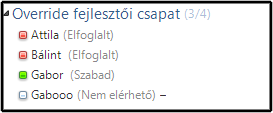
\includegraphics{chapters/chapter02/msn.png}
\caption{MSN csoport a csapatnak}
\label{fig:msn}
\vspace{-20pt}
\end{center}
\end{figure}
\item[Git tároló] A feladatok megoldása közben keletkezett anyagokat egy -- kizárólag a csapat tagjai által hozzáférhető -- helyen tároljuk (lásd fentebb). Így mindig elérhető a fejlesztések legfrissebb változata.
\begin{figure}[h]
\begin{center}
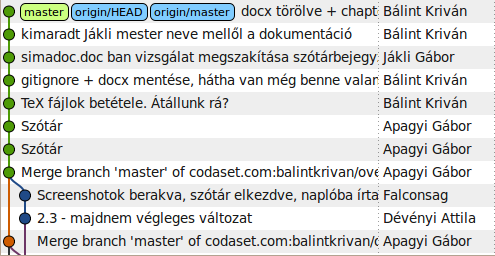
\includegraphics[width=10cm]{chapters/chapter02/git.png}
\caption{Git történet}
\label{fig:git}
\vspace{-20pt}
\end{center}
\end{figure}
\item[Ticket-rendszer] A fejlesztés során felmerülő problémákat, kérdéseket ticket formájában megírjuk egymásnak, amit később a kijelölt felelős személy megold, ha szükséges, akkor együtt konzultálunk a megoldás módjáról, menetéről.
\begin{figure}[h]
\begin{center}
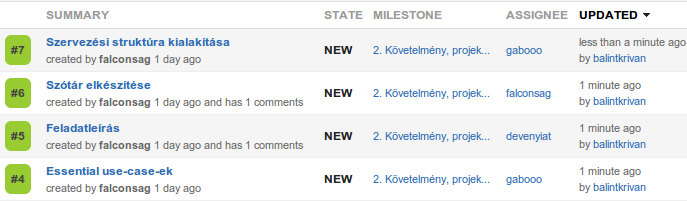
\includegraphics[width=16.7cm]{chapters/chapter02/ticket.png}
\caption{Ticketek}
\label{fig:ticket}
\vspace{-20pt}
\end{center}
\end{figure}
\end{description}

\subsection{Fejlesztési ütemterv}

A program fejlesztésének három fő lépcsőfoka van. Ezek a következők:\\
\textbf{Skeleton}: A cél az, hogy mind a dinamikus, mind az objektum modell jól legyen kitalálva. Ha ezek elkészültek, akkor a fejlesztés szempontjából sikeresen leraktuk az alapokat.\\
\textbf{Prototípus}: Ez már szinte a teljes változat, csak a grafikus felület elemei hiányoznak. Ez a változat tökéletesen megfelelő arra, hogy az objektumok, rutinok, függvények szemantikai helyességét vizsgáljuk.\\
\textbf{Grafikus változat}: A program teljes változata. Tulajdonképpen a prototípus a grafikus felülettel kiegészítve, esetleg kismértékben továbbfejlesztve.

\subsection{Határidők}

\begin{tabular}{l | l}
febr. 11. & Csapat regisztráció \\
febr. 21. & Követelmény, projekt, funkcionalitás \\
febr. 28. & Analízis modell kidolgozása 1. \\
márc. 7. & Analízis modell kidolgozása 2. \\
márc. 14. & Szkeleton tervezése \\
márc. 21. & Szkeleton \\
márc. 28. & Prototípus koncepciója \\
ápr.  4. & Részletes tervek \\
ápr. 18. & Prototípus \\
ápr. 26. & Grafikus felület specifikációja \\
máj. 9. & Grafikus változat \\
máj. 13. & Összefoglalás
\end{tabular}

\section{Feladatleírás}
\label{sec:taskdesc}

Az általunk készített alkalmazás segítségével a felhasználó egy előre elkészített áramköri listából kiválasztott digitális áramkör szimulációját végezheti el grafikus megjelenítéssel. A program az alábbi alkatrészeket támogatja áramköri elemként: ÉS kapu, VAGY kapu, Inverter, Kijelző, Jelgenerátor, Kapcsoló, Vcc és Gnd. Ezek mindegyike egy vagy több ki- és/vagy bemenettel rendelkezik.\\

\noindent A komponensek (alkatrészek) részletezése:

\begin{enumerate}
\item \textbf{Általános komponensek}: A bemenet(ek)re érkező logikai érték(ek) alapján a kimenete(ke)n valamilyen logikai érték(ek)et produkálnak.
\begin{itemize}
\setlength{\itemsep}{0cm}%
\setlength{\parskip}{0cm}%
\item Az ÉS kapu kettő vagy több bemenettel és egy kimenettel rendelkezik. A kimeneten a bemenetre kötött jelek logikai ÉS kapcsolata jelenik meg. 
\item A VAGY kapu kettő vagy több bemenettel és egy kimenettel rendelkezik. A kimeneten a bemenetre kötött jelek logikai VAGY kapcsolata jelenik meg.
\item Az Inverter egyetlen kimenetén az egyetlen bemenetére kötött jel logikai negáltja jelenik meg.
\end{itemize}

\item \textbf{Megjelenítők}: Az ide tartozó elemek feladata a logikai értékek vizualizálása
\begin{itemize}
\setlength{\itemsep}{0cm}%
\setlength{\parskip}{0cm}%
\item A Kijelző komponenssel a felhasználó a bemenetre kötött jelet vizuális formában tudja megjeleníteni.
\end{itemize}

\item \textbf{Jelforrások}: A harmadik csoport elemei melyeknek nincs bemenete csak kimenete, ez vagy előre definiált (gnd és vcc) vagy a felhasználó által módosítható (kapcsoló, jelgenerátor), ezáltal változtatva az áramkör működését.
\begin{itemize}
\setlength{\itemsep}{0cm}%
\setlength{\parskip}{0cm}%
\item Jelgenerátor segítségével egy bitsorozatot tárolhatunk el, amelyet a szimuláció során az egyetlen kimenetén ciklikusan kiad.
\item A Kapcsolónak egy kimenete van, melynek értéke a kapcsoló állásától függ. „Be” állásban igaz, „Ki” állásban hamis értékű.
\item Gnd (,,föld'') konstans 0-át (logikai hamis) kiadó jelforrás.
\item Vcc (,,tápfeszültség'') konstans 1-et (logikai igaz) kiadó jelforrás.
\end{itemize}
\end{enumerate}

Az összes alkatrészre igaz, hogy nem lehet olyan bemenetük, amelyek szabadok, vagyis sehova sincsenek bekötve, ellenkező esetben a szimulációt nem lehet elindítani és a program figyelmezteti erre a felhasználót (ennek elkerülésére, a programmal szállított szimulálható áramkörök egyik komponensének sincs szabad bemenete).

A felhasználó a fentebb említett alkatrészekből összeállított digitális áramkör szimulációját végezheti. Az alkatrészek és azok egymáshoz kötéseik (összeköttetések) grafikus formában kerül megjelenítésre.

A szimuláció során bármelyik komponens pillanatnyi értékeit a felhasználó lekérdezheti az alkatrészre való kattintással, ezzel egyidejűleg a szimulációt szünetelteti. Az áramkör vizsgálata közben a Kapcsolók értékeit szabadon változtathatja, melyek hatása valós időben megjelenik. Szimuláció elkezdésekor az összes áramköri elem kimenete hamis értéket vesz fel. Ha a vizsgálandó áramkör bizonyos idő alatt nem áll be stacionárius állapotba változatlan bemenetek mellett, akkor ez jelzésre kerül a felhasználó számára és a szimuláció automatikusan leáll. A szimuláció bármikor megszakítható majd újraindítható, illetve átválthat egy másik digitális áramkör vizsgálatára (az előre elkészített digitális áramkörök közül választva), amennyiben a jelenlegi áramkört nem kívánja tovább használni.

A szimuláció sebessége a felhasználó által konfigurálható, ezáltal a Jelgenerátor kimenetein kiadott jelek váltakozásának sebessége változtatható.

A Kapcsolók, illetve a Jelgenerátorok gyors és egyszerű alap állapotba helyezése érdekében lehet törölni minden addig elvégzett beállítást egyetlen paranccsal, majd elölről kezdeni az egyes elemek konfigurálását. Lehetőség lesz továbbá a szerkeszthető jelforrások beállításainak elmentésére illetve későbbi visszatöltésére is. A konfiguráció sikeres betöltődéséhez teljesülnie kell annak a feltételnek, hogy abban az összes meghatározott elem szerepeljen az áramkörben, amire használni szeretnénk a beállításokat. Amennyiben ez nem áll fent, akkor a nem specifikált jelforrások alapállapotban lesznek. Előfordulhat még, hogy a konfigurációban olyan elemek szerepelnek, amelyek az áramkörünkben nem, ekkor hibaüzenet jelenik meg és a betöltés megszakad.

\section{Szótár}
\label{sec:dictionary}

\begin{longtable}{r p{10.95cm}}
\textbf{Előre elkészített lista} & Áramköröket tartalmazó előre elkészített gyűjtemény. \\
\textbf{Áramkör} & A komponensek egymáshoz kötéséből létrejövő rendszer. \\
\textbf{Komponens} & Az áramkör alapegysége, mely 3 fajtájú lehet: \emph{általános komponens}, \emph{megjelenítő} és \emph{jelforrás}. \\
\textbf{Alkatrész} & komponens szinonimája\\
\textbf{Általános komponens} & Olyan komponens, mely a bemenet(ek)re érkező logikai érték(ek) alapján a kimenete(ke)n valamilyen logikai érték(ek)et produkál.\\
\textbf{Bemenet} & A komponensek olyan része, melyen keresztül logikai jeleket tudnak fogadni egy másik komponenstől és ezt valamilyen formában felhasználni. \\
\textbf{Logikai jel} & Az áramkörben levő komponensek által továbbított információ a többi komponens számára, mely az igaz illetve a hamis értéket veheti fel.\\
\textbf{Igaz érték} & A kétféle logikai jel egyike. (van amikor az '1'-es szimbólum jelöli)\\
\textbf{Hamis érték} & A kétféle logikai jel egyike. (van amikor a '0'-ás szimbólum jelöli)\\
\textbf{Logikai negált} & Az igaz érték logikai negáltja hamis, hamis értéké pedig igaz.\\
\textbf{Kimenet} & A komponens olyan része, melyen keresztül logikai jeleket tud továbbítani más komponenseknek.\\
\textbf{Jel továbbítás} & A logikai jel egyik komponenstől másik komponensig való áramlása.\\
\textbf{Megjelenítő} & Olyan komponens, mely a bemenet(ek)re érkező logikai jele(ke)t a felhasználó számára érzékelhető módon szemlélteti.\\
\textbf{Jelforrás} & Olyan komponens, mely bemenet nélkül továbbítja az áramkörben specifikált vagy a felhasználó által megadott jele(ek)t a kimenetén további komponens(ek) számára. \\
\textbf{Gnd} & Olyan komponens, mely konstans 0-át ad ki a kimenetén. \\
\textbf{Vcc} & Olyan komponens, mely konstans 1-et ad ki a kimenetén. \\
\textbf{Komponensek egymáshoz kötése} & Egy olyan folyamat, amely során 2 komponenst oly módon kapcso\-lunk össze, hogy az egyik komponens bemenetére a másik komponens kimenetének logikai jelét kapja meg.\\
\textbf{Grafikus megjelenítés} & Az áramkör felhasználó számára felfogható, érzékelhető megjelenítése.\\
\textbf{ÉS kapu} & \emph{Általános komponens}, melynek a bemenetére érkező logikai jelek közt található hamis érték, akkor kimenetén hamis értéket, ellenkező esetben (vagyis minden bemenete logikai igaz) igaz értéket továbbít. \\
\textbf{VAGY kapu} & \emph{Általános komponens}, melynek a bemenetére érkező logikai jelek közt található igaz érték, akkor kimenetén igaz értéket, ellenkező esetben (vagyis minden bemenete logikai hamis) haimis értéket továbbít. \\
\textbf{Inverter} & \emph{Általános komponens}, mely a bemenetére érkező logikai jel negáltját továbbítja a kimenetén. \\
\textbf{Kijelző} & Egy darab logikai jelet váró \emph{megjelenítő}, mely logikai igaz bemenet esetén világít (piros, kék vagy sárga színnel, melyet az áramkör leírója határoz meg), hamis esetén nem. \\
\textbf{Áramkör leíró} & Egy olyan szöveg, mely a program által elvárt módon leírja a teljes áramkört a komponensek és azok összeköttetéseinek definiálásával. \\
\textbf{Jelgenerátor} & Olyan \emph{jelforrás}, mely előre megadott bitsorozatot ad ki ciklikusan a kimenetén.\\
\textbf{Bitsorozat} & Logikai jelekből létrejövő olyan sorozat, melynél az igaz értéket ’1’ szimbólum reprezentál, míg a hamis értéket ’0’.\\
\textbf{Kapcsoló} & Olyan \emph{jelforrás}, mely felhasználói interakció hatására kimenetén igaz, vagy hamis értéket továbbít. \\
\textbf{Felhasználói interakció} & Olyan esemény, melyet a felhasználó saját maga vált ki valamely tevékenysége során, ezzel potenciálisan befolyásolva az áramkör működését. \\
\textbf{Szimuláció} & Az a folyamat, mely során minden alkatrész kimenetének logikai jel értékét kiszámoljuk a bemenetére érkező logikai jelekből, vagy ha \emph{megjelenítő}ről van szó, akkor a felhasználó számára a megjelenítő által meghatározott módon szemléltetjük a bemenetére érkező jeleket. Eközben a felhasználó által megadott időközönként (szimuláció sebessége) léptetjük a jelgenerátort. A szimuláció a felhasználó által indítható és megállítható.\\
\textbf{Jelgenerátor léptetése} & A jelgenerátorban tárolt bitsorozat következő elemére lépünk és azt adjuk ki a kimenetén, ha a végére értünk, akkor előlről indul.\\
\textbf{Szimuláció sebessége} & A jelgenerátor egyes állapotai közötti váltás sebessége. \\
\textbf{Valós időben} & A felhasználó számára lényegében érzékelhetetlen idő alatt.\\
\textbf{Stacionárius} & A rendszer egy stabil állapota, melyben olyan értékek jelennek meg a komponensek kimenetein, amelyek hatására (visszacsatolás esetén sem) változiknak a rendszer komponenseinek kimeneti értékei (Jelgenerátor esetén nincs stacionárius állapot)\\
\textbf{Szimuláció megszakítása/leállítása} & A rendszer komponenseinek állapota nem változik, azok a megszakítás pillanatában felvett értékeket mutatják a következő indításig.\\
\textbf{Állapot} & Az áramkör komponenseinek aktuális tulajdonságainak (kimeneti/bemeneti értékek) összessége \\
\textbf{Alap állapot} & Az a kiindulási állapot, mely az áramkör betöltése után keletkezik. Ilyenkor az \emph{általános komponens}ek kimenetén a hamis érték van.\\
\textbf{Jelforrások konfigurációja} & A szerkeszthető jelforrások beállításainak (kapcsolók állapota, jelgenerátorok bitsorozata stb.) egy állapota.
\end{longtable}

\section{Essential use-case-ek}

\subsection{Use-case diagram}
\label{sec:usecasediagram}

\begin{figure}[H]
\begin{center}
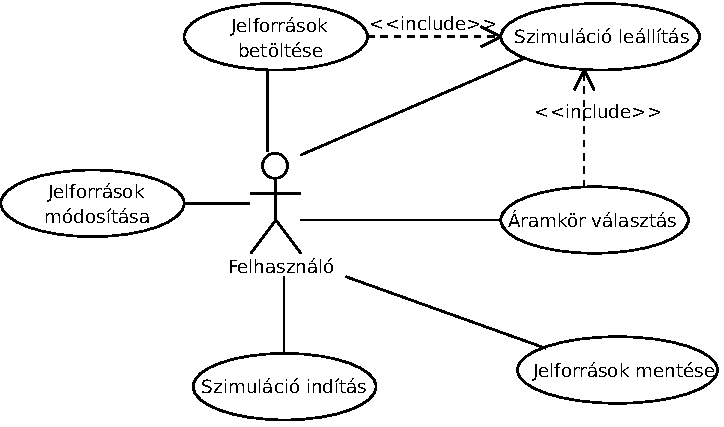
\includegraphics{chapters/chapter02/usecase.pdf}
\caption{Essential use-case diagram}
\label{fig:useCase1}
\end{center}
\end{figure}

\subsection{Use-case leírások}
\label{sec:usecasedesc}

\usecase{Szimuláció leállítás}
{A futó szimuláció leállítása}
{Felhasználó}
{Az éppen futó szimulációt a felhasználó a "Stop" gombbal leállítja.}

\usecase{Szimuláció indítás}
{A áramkör szimulációjának elindítása}
{Felhasználó}
{A felhasználó, az általa korábban kiválasztott áramkör szimulációját a "Start" gombbal elindítja}

\usecase{Áramkör választás}
{Szimulálni kívánt áramkör kiválasztása}
{Felhasználó}
{\vspace{-20pt}\begin{enumerate}
\setlength{\itemsep}{0cm}%
\setlength{\parskip}{0cm}%
\item A felhasználó a Megnyitás menüpontra kapcsol.
\item Kiválaszt egy áramkört a felkínált listából.
\item Az áramkör betöltődik a rendszerbe.
\end{enumerate}\vspace{-20pt}}

\usecase{Jelforrások betöltése}
{Az áramkör jelforrásainak betöltése}
{Felhasználó}
{\vspace{-20pt}\begin{enumerate}
\setlength{\itemsep}{0cm}%
\setlength{\parskip}{0cm}%
\item A felhasználó a "Jelforrások betöltése" menüpontra kapcsol.
\item Megadja, hogy melyik fájlt olvassa be a rendszer.
\item Ha a fájl megfelelő, akkor a betöltés megtörténik, egyéb esetben a felhasználót figyelmeztetjük.
\end{enumerate}\vspace{-20pt}}

\usecase{Jelforrások mentése}
{Az áramkör jelforrásainak mentése}
{Felhasználó}
{\vspace{-20pt}\begin{enumerate}
\setlength{\itemsep}{0cm}%
\setlength{\parskip}{0cm}%
\item A felhasználó a "Jelforrások mentése" menüpontra kapcsol.
\item Megadja, hogy melyik fájlba történjen a mentés.
\item A mentés megtörténik, amennyiben ez valami oknál fogva nem sikerült (nincs joga, nincs elég terület stb.), a felhasználót figyelmeztetjük.
\end{enumerate}\vspace{-20pt}}


%% Szglab4
% ===========================================================================
%
\section{Napló}

\begin{naplo}

\bejegyzes
{2011.02.15.~21:30~}
{2 óra}
{Kriván B.\newline
Dévényi A.\newline
Jákli G.}
{Értekezlet.\newline
Döntések: Megegyeztünk a feladat értelme\-zését illetően.
Milyen kérdéseket teszünk fel a konzulensnek az első konzultáción?\newline
Ezeket a Apagyi G. és Péter T. számára továbbítottuk.}

\bejegyzes
{2011.02.16.~09:00~}
{2 óra}
{Kriván B.\newline
Dévényi A.\newline
Apagyi G.\newline
Péter T.}
{Értekezlet.\newline
Döntések:
\begin{itemize}
\setlength{\itemsep}{0cm}%
\setlength{\parskip}{0cm}%
\item Fejlesztői környezetben megállapodtunk (\ref{sec:devenvironment})
\item Projekt szervezési struktúráját rögzítettük (\ref{sec:orgstructure})
\item A felmerülő algoritmusokról is konzultáltunk.
\end{itemize}
}

\bejegyzes
{2011.02.16.~15:00~}
{1 óra}
{Jákli G.}
{Tevékenység: Projekt terv bővítése, formázá\-sa, javítása (\ref{sec:projectplan})}

\bejegyzes
{2011.02.17.~16:00~}
{1 óra}
{Jákli G.\newline
Kriván B.\newline
Dévényi A.}
{Tevékenység: \aref{sec:reqdef} és \aref{sec:projectplan} alfejezet közös átdolgozása}

\bejegyzes
{2011.02.17.~19:15~}
{45 perc}
{Jákli G.\newline
Kriván B.\newline
Dévényi A.}
{Értekezlet.\newline
Döntések: \Aref{sec:taskdesc} alfejezet főbb gondolatait megfogalmaztuk, és meghatároztuk, hogy mik legyenek a mindenképpen lejegyezendő dolgok.}

\bejegyzes
{2011.02.17.~20:00~}
{50 perc}
{Jákli G.}
{Tevékenység: A megbeszéltek alapján el\-kezdte \aref{sec:taskdesc} alfejezet megírását.}

\bejegyzes
{2011.02.17.~23:00~}
{30 perc}
{Péter T.}
{Tevékenység: Szervezési struktúra kiegészí\-tése képernyőképekkel}

\bejegyzes
{2011.02.18.~00:00~}
{30 perc}
{Kriván B.\newline
Dévényi A.\newline
Péter T}
{Értekezlet (Msn megbeszélés).\newline
Döntések: \Aref{sec:taskdesc} alfejezet módosításának elhatározása és a szótárba (\ref{sec:dictionary}) bekerülő szavak rögzítése}

\bejegyzes
{2011.02.18.~00:30~}
{30 perc}
{Péter T.}
{Az előző értekezleten meghatározott szavak felvétele a szótárba, még csak felsorolás szint\-jén}

\bejegyzes
{2011.02.18.~14:00~}
{1 óra}
{Péter T.}
{Szótárban lévő szavak magyarázatainak kitöl\-tése}

\bejegyzes
{2011.02.18.~15:30~}
{30 perc}
{Apagyi G.}
{Szótárban lévő szavak megmagyarázásának folytatása}

\bejegyzes
{2011.02.19.~12:00~}
{2 óra}
{Kriván B.}
{Tevékenység: helyesírási hibák javítása, szó\-tár (\ref{sec:dictionary}) szerkesztése (sorrendek változtatása, további szavak bevezetése, meglévők magya\-rázatainak szerkesztése)}

\bejegyzes
{2011.02.19.~19:30~}
{30 perc}
{Kriván B.\newline
Jákli G.}
{Értekezlet (Msn megbeszélés).\newline
Döntések: Új essential use-caset kell rajzolni. Szükség van Gnd és Vcc komponensre.}

\bejegyzes
{2011.02.19.~20:00~}
{30 perc}
{Jákli G.}
{Új essential use-case megrajzolása (\ref{sec:usecasediagram}), use-case leírások megírása (\ref{sec:usecasedesc})}

\bejegyzes
{2011.02.19.~20:00~}
{30 perc}
{Kriván B.}
{Gnd és Vcc komponens felvétele (\ref{sec:taskdesc}), megfelelő részek szerkesztése, use-case konvertálása \LaTeX{}-kompatibilis formátumba és felvétele a dokumentációba}

\end{naplo}



%\setcounter{chapter}{2}
%% Szglab4
% ===========================================================================
%
\chapter{Analízis modell kidolgozása 1}

\thispagestyle{fancy}

\section{Objektum katalógus}

\comment{Minden, a feladatban szereplő objektum rövid, egy-két bekezdés hosszú ismertetése. Meg kell jelenjen minden objektumhoz, hogy mi a felelőssége. Informális leírás, ezért nem kell foglalkozni az örökléssel, az interfészekkel, az absztrakt osztályokkal, a segédosztályokkal.}

\subsection{Objektum1}
\comment{Felelősség informális leírása}

\subsection{Objektum2}
\comment{Felelősség informális leírása}

\section{Osztályok leírása}
\comment{Az előző alfejezetben tárgyalt objektumok felelősségének formalizálása attribútumokká, metódusokká. Csak publikus metódusok szerepelhetnek. Ebben az alfejezetben megjelennek az interfészek, az öröklés, az absztrakt osztályok. Segédosztályokra még mindig nincs szükség. Az osztályok ABC sorrendben kövessék egymást. Interfészek esetén az Interfészek, Attribútumok pontok kimaradnak.}

\subsection{Osztály1}
\begin{itemize}
\item Felelősség\\
\comment{Mi az osztály felelőssége. Kb 1 bekezdés.}
\item Ősosztályok\\
\comment{Mely osztályokból származik (öröklési hierarchia)\newline
Legősebb osztály $\rightarrow$ Ősosztály2 $\rightarrow$ Ősosztály3...}
\item Interfészek\\
\comment{Mely interfészeket valósítja meg.}
\item Attribútumok\\
\comment{Milyen attribútumai vannak}
	\begin{itemize}
		\item attribútum1: attribútum jellemzése: mire való
		\item attribútum2: attribútum jellemzése: mire való
	\end{itemize}
\item Metódusok\\
\comment{Milyen publikus metódusokkal rendelkezik. Metódusonként egy-három mondat arról, hogy a metódus mit csinál.}
	\begin{itemize}
		\item int foo(Osztály3 o1, Osztály4 o2): metódus leírása
		\item int bar(Osztály5 o1): metódus leírása
	\end{itemize}
\end{itemize}

\subsection{Osztály2}
\begin{itemize}
\item Felelősség\\
\comment{Mi az osztály felelőssége. Kb 1 bekezdés.}
\item Ősosztályok\\
\comment{Mely osztályokból származik (öröklési hierarchia)\newline
Legősebb osztály $\rightarrow$ Ősosztály2 $\rightarrow$ Ősosztály3...}
\item Interfészek\\
\comment{Mely interfészeket valósítja meg.}
\item Attribútumok\\
\comment{Milyen attribútumai vannak}
	\begin{itemize}
		\item attribútum1: attribútum jellemzése: mire való
		\item attribútum2: attribútum jellemzése: mire való
	\end{itemize}
\item Metódusok\\
\comment{Milyen publikus metódusokkal rendelkezik. Metódusonként egy-három mondat arról, hogy a metódus mit csinál.}
	\begin{itemize}
		\item int foo(Osztály3 o1, Osztály4 o2): metódus leírása
		\item int bar(Osztály5 o1): metódus leírása
	\end{itemize}
\end{itemize}

\section{Statikus struktúra diagramok}
\comment{Az előző alfejezet osztályainak kapcsolatait és publikus metódusait bemutató osztálydiagram(ok). Tipikus hibalehetőségek: csillag-topológia, szigetek.}

\begin{figure}[h]
\begin{center}
%\includegraphics[width=17cm]{chapters/chapter03/example.pdf}
\caption{x}
\label{fig:example1}
\end{center}
\end{figure}

\section{Szekvencia diagramok}
\comment{Inicializálásra, use-case-ekre, belső működésre. Konzisztens kell legyen az előző alfejezettel. Minden metódus, ami ott szerepel, fel kell tűnjön valamelyik szekvenciában. Minden metódusnak, ami szekvenciában szerepel, szereplnie kell a valamelyik osztálydiagramon.}

\begin{figure}[h]
\begin{center}
%\includegraphics[width=17cm]{chapters/chapter03/example.pdf}
\caption{x}
\label{fig:example2}
\end{center}
\end{figure}

\section{State-chartok}
\comment{Csak azokhoz az osztályokhoz, ahol van értelme. Egyetlen állapotból álló state-chartok ne szerepeljenek. A játék működését bemutató state-chart-ot készíteni tilos.}

\begin{figure}[h]
\begin{center}
%\includegraphics[width=17cm]{chapters/chapter03/example.pdf}
\caption{x}
\label{fig:example3}
\end{center}
\end{figure}


%% Szglab4
% ===========================================================================
%
\section{Napló}

\begin{naplo}

\bejegyzes
{2010.03.21.~18:00~} % Kezdet
{2,5 óra} % Időtartam
{Horváth\newline
Németh\newline
Tóth\newline
Oláh} % Résztvevők
{Értekezlet. Döntés: Horváth elkészíti az osztálydiagramot, Oláh a use-case leírásokat.} % Leírás

\bejegyzes
{2010.03.23.~23:00~}
{5 óra}
{Németh}
{Tevékenység: Németh implementálja a tesztelő programokat.}

\bejegyzes
{...}
{...}
{...}
{...}


\end{naplo}



%\setcounter{chapter}{3}
%% Szglab4
% ===========================================================================
%
\chapter{Analízis modell kidolgozása 2}

\thispagestyle{fancy}

\section{Objektum katalógus}

\subsection{\bf Parser}
Áramkör értelmező objektum, feladata, hogy a paraméterként átadott, illetve fájlban elhelyezett komponenseket értelmezze, a kapcsolatokat feltérképezze, elvégezze az összeköttetéseket, és ezáltal felépítse az áramkört.

\subsection{\bf Simulation}
Szimuláció objektum. A szimulációért felelős. Elindítja a jelgenerátor léptetőt, s utasítja az áramkört több kiértékelési ciklus lefuttatásához, amíg az áramkörben van változás. Ha a változás megadott lépésen belül nem áll meg, tájékoztatja a felhasználót, hogy nincs stacionárius állapot. Amikor leállítódik, a jelgenerátor-léptetőt is leállítja.

\subsection{\bf Circuit}
Az áramkör objektum. Ezen objektum feladata a jelgenerátor léptető kérésére a jelgenerátorok léptetése, az áramkörben található komponensek utasítása arra, hogy töröljék a "már kiértékelve" flaget egy adott kiértékelési ciklus előtt, hogy ezáltal a ciklusban minden kimenet értéke frissülhessen.
Továbbá feladata a kiértékelés elindítása az összes kijelzőre, mert a rendszer kiértékelése a kijelzők kiértékelésével kezdődik.

\subsection{\bf SequenceGeneratorStepper}
Jelgenerátor léptető objektum. Feladata, hogy az áramkört utasítsa a jelgenerátorok léptesésére.

\subsection{\bf SequenceGenerator}
Jelgenerátor, az áramkört felépítő egyik alapelem, kiértékelési kezdeményezés hatására az előre betáplált jelsorozatot soron következő elemét állítja be aktuális értékként, így azon komponensek melyek bemenetére a Jelgenerátor van kötve, elérik aktuális értékét. Bemenete nem komponens jellegű így nem kezel más komponenseket. Mikor az áramkör kéri tőle, hogy lépjen, akkor a bitsorozat következő elemére lép.

\subsection{\bf AndGate}
ÉS kapu, az áramkör egyik alapeleme. Bemeneteire kötött komponensek kiértékelését kezdeményezi, s a kapott értékek logikai ÉS kapcsolatát valósítja meg, amit a kimenetén kiad.

\subsection{\bf OrGate}
VAGY kapu, az áramkör egyik alapeleme. Bemeneteire kötött komponensek kiértékelését kezdeményezi, s a kapott értékek logikai VAGY kapcsolatát valósítja meg, amit a kimenetén kiad.

\subsection{\bf Inverter}
Invertáló, az áramkör alapelemei közé tartozik. A bemenetére érkező jel logikai negáltját valósítja meg, amit a kimenetén kiad.

\subsection{\bf Gnd}
Föld, az áramkört felépítő egyik elem, állandó értéke logikai hamis. Bemenete nem létezik, így nem kezdeményez további kiértékeléseket.

\subsection{\bf Vcc}
Tápfeszültség, az áramkör egyik alapeleme, mely állandóan a logikai igazt adja ki a kimenetén.

\subsection{\bf Led}
Egy kijelző az áramkör alapeleme, bemenetére kötött komponens kiértékelését kezdeményezi, és ezáltal az aktuális értékét egy a felhasználó számára érzékelhető módon kijelzi.

\subsection{\bf Toggle}
Kapcsoló, az áramkört felépítő elem, felhasználói interakciót követően, az aktuális értékét lehet állítani. Komponens bemenete nincs, így nem kezel további komponenseket.

\subsection{\bf Value}
A logikai értékeket megvalósító objektum. Jelenleg két érték lehetséges: logikai igaz, logikai hamis.

\subsection{\bf FlipFlopD}
D flip flopot megvalósító objektum. Csak akkor lép működésbe, mikor az órajelbemenetén a logikai érték hamisról igazra változik, ekkor az értékbemenettől függően változtatja a kimeneti értékét.

\subsection{\bf FlipFlopJK}
JK flip flopot megvalósító objektum. Csak akkor lép működésbe, mikor az órajelbemenetén a logikai érték hamisról igazra változik, ekkor az értékbemenetektől függően változtatja a kimeneti értékét.

\subsection{\bf Mpx}
4-1-es multiplexer áramköri építőelemet megvalósító objektum. Bemeneteire kötött komponensek kiértékelését kezdeményezi, a választó bemenet függvényében adja ki a kimeneten az egyik, vagy másik értékbemenetére kötött értéket.

\subsection{\bf SevenSegmentDisplay}
Hétszegmenses kijelző objektuma. Minden bemenete egy-egy szegmensért felelős, melyek 8-as alakban helyezkednek el.

\subsection{\bf SourceWriter}
Ez az objektum végzi el a konfigurálható elemek beállításainak fájlba írását a felhasználó kérésére.

\subsection{\bf SourceReader}
Ez az objektum végzi el a konfigurálható elemek beállításainak fájlból beolvasását a felhasználó kérésére.

\section{Osztályok leírása}

\subsection{Circuit}
\begin{itemize}
\item Felelősség\\
Áramkört reprezentál, melyhez komponeseket lehet adni, és kiértékelési ciklusokat  lehet futtatni, utóbbi a \texttt{Simulation} feladata.
\item Ősosztályok\ Object $\rightarrow{}$ Circuit.
\item Interfészek (nincs)
\item Attribútumok $\ $
\begin{itemize}
	\item \texttt{private HashMap componentMap} 
 % TODO
	\item \texttt{private Simulation simulation} 
 % TODO
	\item \texttt{private boolean stable} 
 % TODO
\end{itemize}
\item Metódusok$\ $
\begin{itemize}
	\item \texttt{public Component addComponent(Component component)}: Komponens hozzáadása az áramkörhöz.
	\item \texttt{public void doEvaluationCycle()}: Egy kiértékelési ciklus lefuttatása. Az áramkörtől ezután lekérdezhető, hogy  stabil (nem változott semelyik komponens kimenete az utolsó futtatás óta)  vagy instabil állapotban van-e.
	\item \texttt{public Component getComponentByName(String name)}: Lekérünk egy komponenst az áramkörtől a neve alapján.
	\item \texttt{public List getDisplays()}: Megjelenítő típusú komponeseket adja vissza.
	\item \texttt{public List getSources()}: Jelforrás típusú komponenseket adja vissza.
	\item \texttt{public boolean isStable()}: Áramkör stacionárius állapotának lekérdezése.
	\item \texttt{public void setSimulation(Simulation simulation)}: Szimuláció beállítása.
	\item \texttt{public void setStable(boolean stable)}: Áramkör stabilitásának beállítása.
	\item \texttt{public void simulationRefreshRequired()}: Jelzi a szimuláció felé, hogy új ciklust kell indítani. Ezt egy jelforrás  beállítása után hívjuk meg.
	\item \texttt{public void stepGenerators()}: Jelgenerátorok a szimuláció szemszögéből nézve, egyszerre történő  léptetése.
\end{itemize}
\end{itemize}

\subsection{LogSim}
\begin{itemize}
\item Felelősség\\

 % TODO
\item Ősosztályok\ Object $\rightarrow{}$ LogSim.
\item Interfészek (nincs)
\item Attribútumok $\ $
\begin{itemize}
\item (nincs)
\end{itemize}
\item Metódusok$\ $
\begin{itemize}
	\item \texttt{public static void main(String[] args)}: 
 % TODO
\end{itemize}
\end{itemize}

\subsection{SequenceGeneratorStepper}
\begin{itemize}
\item Felelősség\\

 % TODO
\item Ősosztályok\ Object $\rightarrow{}$ Thread $\rightarrow{}$ SequenceGeneratorStepper.
\item Interfészek (nincs)
\item Attribútumok $\ $
\begin{itemize}
	\item \texttt{private long pause} 
 % TODO
	\item \texttt{private boolean shouldRun} 
 % TODO
	\item \texttt{private Simulation simulation} 
 % TODO
\end{itemize}
\item Metódusok$\ $
\begin{itemize}
	\item \texttt{public void run()}: 
 % TODO
\end{itemize}
\end{itemize}

\subsection{Value}
\begin{itemize}
\item Felelősség\\
Az áramkörben előfordulható érték
\item Ősosztályok\ Object $\rightarrow{}$ Enum $\rightarrow{}$ Value.
\item Interfészek (nincs)
\item Attribútumok $\ $
\begin{itemize}
	\item \texttt{public static final Value FALSE} 
 % TODO
	\item \texttt{public static final Value TRUE} 
 % TODO
\end{itemize}
\item Metódusok$\ $
\begin{itemize}
	\item \texttt{public Value invert()}: 
 % TODO
	\item \texttt{public static Value valueOf(String name)}: 
 % TODO
	\item \texttt{public static Value[] values()}: 
 % TODO
\end{itemize}
\end{itemize}


\subsection{Component}
Absztrakt osztály.
\begin{itemize}
\item Felelősség\\

 % TODO
\item Ősosztályok\ Object $\rightarrow{}$ Component.
\item Interfészek (nincs)
\item Attribútumok $\ $
\begin{itemize}
	\item \texttt{protected boolean alreadyEvaluated} 
 % TODO
	\item \texttt{protected Circuit circuit} 
 % TODO
	\item \texttt{protected Value[] currentValue} 
 % TODO
	\item \texttt{protected int[] indices} 
 % TODO
	\item \texttt{protected Component[] inputs} 
 % TODO
	\item \texttt{protected Value[] lastValue} 
 % TODO
	\item \texttt{protected String name} 
 % TODO
\end{itemize}
\item Metódusok$\ $
\begin{itemize}
	\item \texttt{public void clearEvaluatedFlag()}: 
 % TODO
	\item \texttt{public Value evaluate()}: 
 % TODO
	\item \texttt{public Value evaluate(int outputPin)}: Számolás:
	\item \texttt{public String getName()}: 
 % TODO
	\item \texttt{public Value getValue()}: 
 % TODO
	\item \texttt{public Value getValue(int idx)}: 
 % TODO
	\item \texttt{public void setCircuit(Circuit parent)}: 
 % TODO
	\item \texttt{public void setInput(int inputSlot, Component component)}: 
 % TODO
	\item \texttt{public void setInput(int inputPin, Component component, int outputPin)}: Beállítunk egy bemenetet.
	\item \texttt{public void setInputPinsCount(int inputPinsCount)}: 
 % TODO
	\item \texttt{public void setName(String name)}: 
 % TODO
\end{itemize}
\end{itemize}

\subsection{IsDisplay}
Interfész.
\begin{itemize}
\item Felelősség\\

 % TODO
\item Ősosztályok\ IsDisplay.
\item Interfészek (nincs)
\item Metódusok$\ $
\begin{itemize}
\item (nincs)
\end{itemize}
\end{itemize}

\subsection{IsSource}
Interfész.
\begin{itemize}
\item Felelősség\\

 % TODO
\item Ősosztályok\ IsSource.
\item Interfészek (nincs)
\item Metódusok$\ $
\begin{itemize}
	\item \texttt{public void setValues(Value[] values)}: Beállítjuk a jelforrás értékét.
\end{itemize}
\end{itemize}


\subsection{AndGate}
\begin{itemize}
\item Felelősség\\
ÉS kapu, az áramkör egyik alapeleme. Bemeneteire kötött komponensek  kiértékelését kezdeményezi, s a kapott értékek logikai ÉS kapcsolatát  valósítja meg, amit a kimenetén kiad.
\item Ősosztályok:\ Object $\rightarrow{}$ AbstractComponent $\rightarrow{}$ AndGate.
\item Interfészek: (nincs)
\item Attribútumok $\ $
\begin{itemize}
\item (nincs)
\end{itemize}
\item Metódusok$\ $
\begin{itemize}
\item (nincs)
\end{itemize}
\end{itemize}

\subsection{FlipFlopD}
\begin{itemize}
\item Felelősség\\
D flipflop, mely felfutó órajelnél beírja a belső memóriába az adatbemeneten (D)  lévő értéket.
\item Ősosztályok:\ Object $\rightarrow{}$ AbstractComponent $\rightarrow{}$ FlipFlop $\rightarrow{}$ FlipFlopD.
\item Interfészek: (nincs)
\item Attribútumok $\ $
\begin{itemize}
\item (nincs)
\end{itemize}
\item Metódusok$\ $
\begin{itemize}
\item (nincs)
\end{itemize}
\end{itemize}

\subsection{FlipFlopJK}
\begin{itemize}
\item Felelősség\\
JK flipflop, mely a belső memóriáját a Követelmények résznél leírt módon  a J és K bemenetektől függően változtatja.
\item Ősosztályok:\ Object $\rightarrow{}$ AbstractComponent $\rightarrow{}$ FlipFlop $\rightarrow{}$ FlipFlopJK.
\item Interfészek: (nincs)
\item Attribútumok $\ $
\begin{itemize}
\item (nincs)
\end{itemize}
\item Metódusok$\ $
\begin{itemize}
\item (nincs)
\end{itemize}
\end{itemize}

\subsection{Gnd}
\begin{itemize}
\item Felelősség\\
A "föld" komponens, mely állandóan a hamis értéket adja ki. Nincs bemenete.
\item Ősosztályok:\ Object $\rightarrow{}$ AbstractComponent $\rightarrow{}$ Gnd.
\item Interfészek: (nincs)
\item Attribútumok $\ $
\begin{itemize}
\item (nincs)
\end{itemize}
\item Metódusok$\ $
\begin{itemize}
\item (nincs)
\end{itemize}
\end{itemize}

\subsection{Inverter}
\begin{itemize}
\item Felelősség\\
Inverter alkatrész, mely invertálva adja ki a kimenetén a bemenetén  érkező jelet.
\item Ősosztályok:\ Object $\rightarrow{}$ AbstractComponent $\rightarrow{}$ Inverter.
\item Interfészek: (nincs)
\item Attribútumok $\ $
\begin{itemize}
\item (nincs)
\end{itemize}
\item Metódusok$\ $
\begin{itemize}
\item (nincs)
\end{itemize}
\end{itemize}

\subsection{Led}
\begin{itemize}
\item Felelősség\\
Egy LED-et reprezentál, mely világít, ha bemenetén igaz érték van.  3 féle színe lehet, ezeket a Color enumeráció határozza meg.
\item Ősosztályok:\ Object $\rightarrow{}$ AbstractComponent $\rightarrow{}$ Led.
\item Interfészek: IsDisplay.
\item Attribútumok $\ $
\begin{itemize}
\item (nincs)
\end{itemize}
\item Metódusok$\ $
\begin{itemize}
\item (nincs)
\end{itemize}
\end{itemize}

\subsection{Mpx}
\begin{itemize}
\item Felelősség\\
4-1-es multiplexer, melynek a bemeneti lábak sorrendje a következő:  D0, D1, D2, D3, S0, S1. Ahol Dx az adatbemenetek, Sy a kiválasztóbemenetek.  Kimenetén a kiválasztóbemenetektől függően valamelyik adatbemenet kerül kiadásra.
\item Ősosztályok:\ Object $\rightarrow{}$ AbstractComponent $\rightarrow{}$ Mpx.
\item Interfészek: (nincs)
\item Attribútumok $\ $
\begin{itemize}
\item (nincs)
\end{itemize}
\item Metódusok$\ $
\begin{itemize}
\item (nincs)
\end{itemize}
\end{itemize}

\subsection{OrGate}
\begin{itemize}
\item Felelősség\\
VAGY kapu, az áramkör egyik alapeleme. Bemeneteire kötött komponensek  kiértékelését kezdeményezi, s a kapott értékek logikai VAGY kapcsolatát  valósítja meg, amit a kimenetén kiad.
\item Ősosztályok:\ Object $\rightarrow{}$ AbstractComponent $\rightarrow{}$ OrGate.
\item Interfészek: (nincs)
\item Attribútumok $\ $
\begin{itemize}
\item (nincs)
\end{itemize}
\item Metódusok$\ $
\begin{itemize}
\item (nincs)
\end{itemize}
\end{itemize}

\subsection{SequenceGenerator}
\begin{itemize}
\item Felelősség\\
Jelgenerátort reprezentál, amely a beállított bitsorozatot adja ki. A  SequenceGeneratorStepper feladata, hogy a step() metódust meghívja ezen osztály  példányain. Azokat a FF-eket vezérli, melyek CLK bemenetére ez a komponens van kötve,  vagyis ha éppen felfutó él jön, akkor ezeket engedélyezi különben nem.
\item Ősosztályok:\ Object $\rightarrow{}$ AbstractComponent $\rightarrow{}$ SequenceGenerator.
\item Interfészek: IsSource.
\item Attribútumok $\ $
\begin{itemize}
	\item \texttt{private List ffList}: Azon FF-ek listája, melyekre ez a jelgenerátor van bekötve a CLK bemenetre.
	\item \texttt{private int index}: Bitsorozat egy indexe, ez határozza meg, hogy éppen melyik értéket adja ki.
	\item \texttt{private Value[] sequence}: Tárolt bitsorozat
\end{itemize}
\item Metódusok$\ $
\begin{itemize}
	\item \texttt{void addFlipFlop(FlipFlop ff)}: A flipflop-ot feliratkoztatjuk a jelgenerátorhoz, így ha felfutó él lesz,  akkor tudunk neki jelezni.
	\item \texttt{Value[] getValues()}: Jelgenerátor bitsorozatának lekérdezése
	\item \texttt{void setValues(Value[] values)}: Jelgenerátor bitsorozatának beállítása
	\item \texttt{void step()}: A jelgenerátor lép, a bitsorozat következő elemére ugrik. A következő léptetésig  ez kerül kiadásra a kimeneteken.
\end{itemize}
\end{itemize}

\subsection{SevenSegmentDisplay}
\begin{itemize}
\item Felelősség\\
7-szegmenses kijelzőt reprezentál, melynek 7 bemenete vezérli a  megfelelő szegmenseket, ezek világítanak, ha az adott bemenetre logikai  igaz van kötve.
\item Ősosztályok:\ Object $\rightarrow{}$ AbstractComponent $\rightarrow{}$ SevenSegmentDisplay.
\item Interfészek: IsDisplay.
\item Attribútumok $\ $
\begin{itemize}
\item (nincs)
\end{itemize}
\item Metódusok$\ $
\begin{itemize}
\item (nincs)
\end{itemize}
\end{itemize}

\subsection{Toggle}
\begin{itemize}
\item Felelősség\\
Kapcsoló jelforrás, melyet a felhasználó szimuláció közben kapcsolgathat.
\item Ősosztályok:\ Object $\rightarrow{}$ AbstractComponent $\rightarrow{}$ Toggle.
\item Interfészek: IsSource.
\item Attribútumok $\ $
\begin{itemize}
\item (nincs)
\end{itemize}
\item Metódusok$\ $
\begin{itemize}
	\item \texttt{Value[] getValues()}: Lekérjük a kapcsoló értékét (1 elemű tömb)
	\item \texttt{void setValues(Value[] values)}: Kapcsoló állapotának változtatása, csak 1 elemű tömböt kaphat paraméterül.
\end{itemize}
\end{itemize}

\subsection{Vcc}
\begin{itemize}
\item Felelősség\\
A tápfeszültés komponens, ami konstans igaz értéket ad. Nincs bemenete.
\item Ősosztályok:\ Object $\rightarrow{}$ AbstractComponent $\rightarrow{}$ Vcc.
\item Interfészek: (nincs)
\item Attribútumok $\ $
\begin{itemize}
\item (nincs)
\end{itemize}
\item Metódusok$\ $
\begin{itemize}
\item (nincs)
\end{itemize}
\end{itemize}


\subsection{Parser}
\begin{itemize}
\item Felelősség\\

 % TODO
\item Ősosztályok\ Object $\rightarrow{}$ Parser.
\item Interfészek (nincs)
\item Attribútumok $\ $
\begin{itemize}
	\item \texttt{private static final HashMap availableComponents} 
 % TODO
	\item \texttt{private Circuit circuit} 
 % TODO
	\item \texttt{private static Pattern componentPattern} 
 % TODO
	\item \texttt{private int constComps} 
 % TODO
	\item \texttt{private static Pattern inputPattern} 
 % TODO
	\item \texttt{private HashMap inputs} 
 % TODO
\end{itemize}
\item Metódusok$\ $
\begin{itemize}
	\item \texttt{public Circuit parse(File file)}: Létrehoz egy áramkört a megadott fájlból
	\item \texttt{public Circuit parse(String[] content)}: Létrehoz egy áramkört az argumentumokban megadott komponensekből
\end{itemize}
\end{itemize}

\subsection{SourceWriter}
\begin{itemize}
\item Felelősség\\
Kiírja egy fájlba a jelforrásokat
\item Ősosztályok\ Object $\rightarrow{}$ SourceWriter.
\item Interfészek (nincs)
\item Attribútumok $\ $
\begin{itemize}
\item (nincs)
\end{itemize}
\item Metódusok$\ $
\begin{itemize}
	\item \texttt{public void add(IsSource source)}: Hozzáadjuk a fájlhoz az adott jelforrás beállítását
	\item \texttt{public void close()}: Bezárjuk a fájlt.
\end{itemize}
\end{itemize}



\section{Statikus struktúra diagramok}

\begin{figure}[H]
\begin{center}
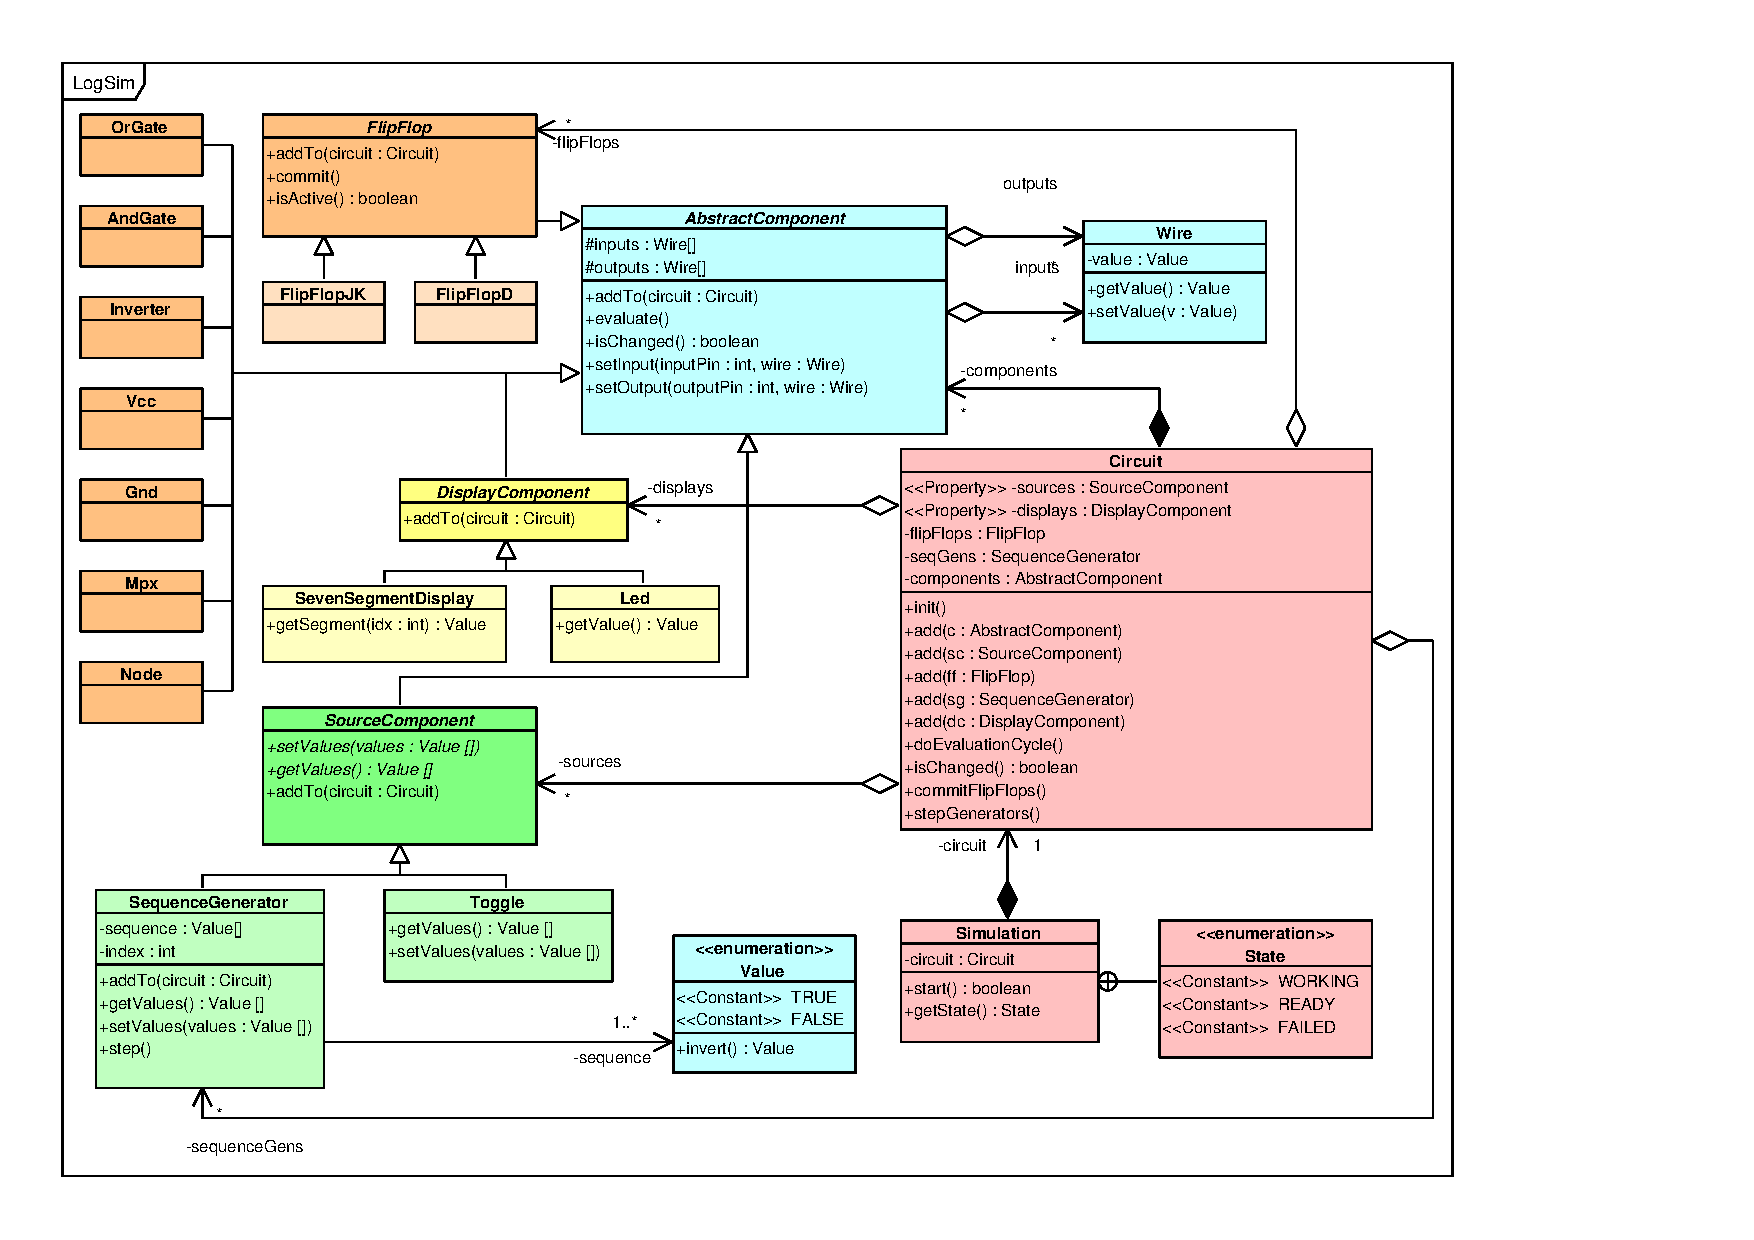
\includegraphics[angle=90, width=17cm]{chapters/chapter04/classdiagram/class.pdf}
\caption{Statikus struktúra nézet}
\label{fig:class_diagram}
\end{center}
\end{figure}
%
%\begin{figure}[H]
%\begin{center}
%\includegraphics*[angle=90, width=14cm, viewport = 765 475 1530 930]{chapters/chapter03/classdiagram/class_diagram.pdf}
%\caption{Statikus struktúra nézet (jobb felső)}
%\label{fig:class_diagram}
%\end{center}
%\end{figure}
%
%\begin{figure}[H]
%\begin{center}
%\includegraphics*[angle=90, width=14cm, viewport = 0 0 765 475]{chapters/chapter03/classdiagram/class_diagram.pdf}
%\caption{Statikus struktúra nézet (bal alsó)}
%\label{fig:class_diagram}
%\end{center}
%\end{figure}
%
%\begin{figure}[H]
%\begin{center}
%\includegraphics*[angle=90, width=14cm, viewport = 765 0 1530 475]{chapters/chapter03/classdiagram/class_diagram.pdf}
%\caption{Statikus struktúra nézet (jobb alsó)}
%\label{fig:class_diagram}
%\end{center}
%\end{figure}

\section{Szekvencia diagramok}

\begin{figure}[H]
\begin{center}
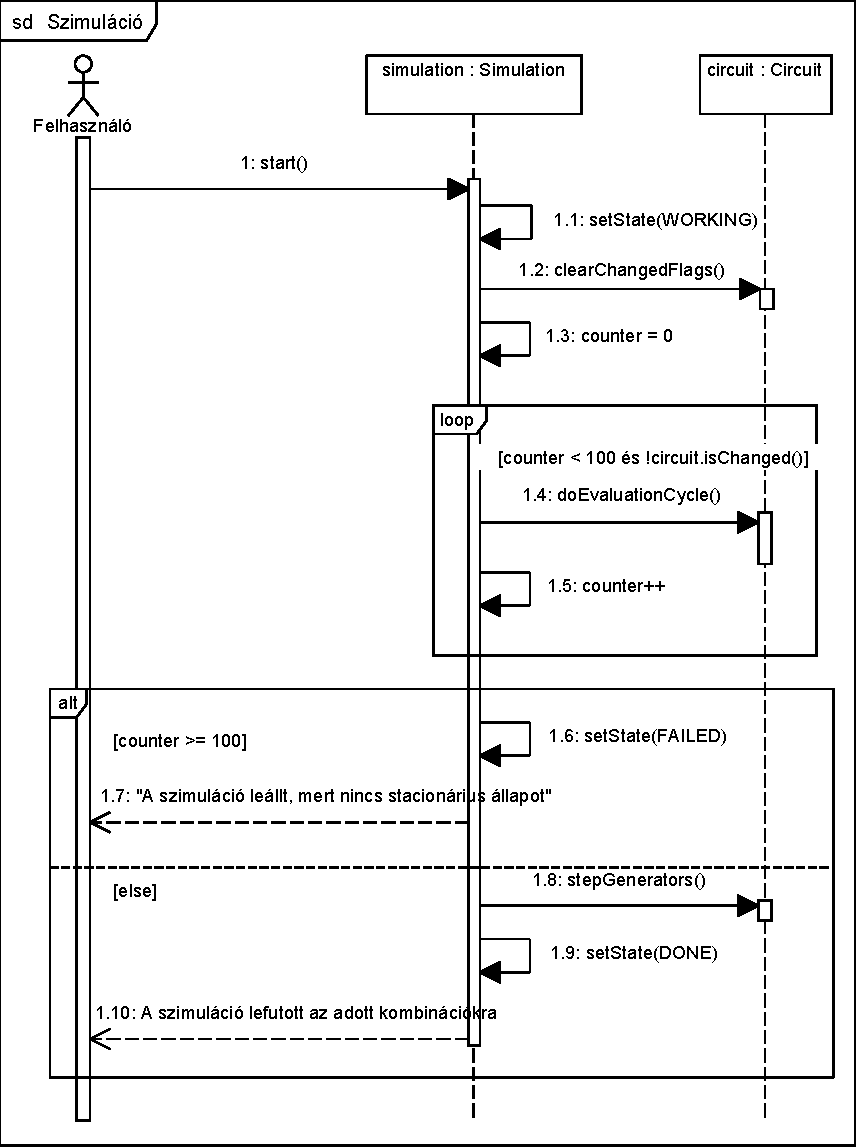
\includegraphics{chapters/chapter04/seqdiagrams/felhasznalo_szimulacio.pdf}
\caption{Szimuláció futás közben}
\label{fig:user_sim}
\end{center}
\end{figure}

\begin{figure}[H]
\begin{center}
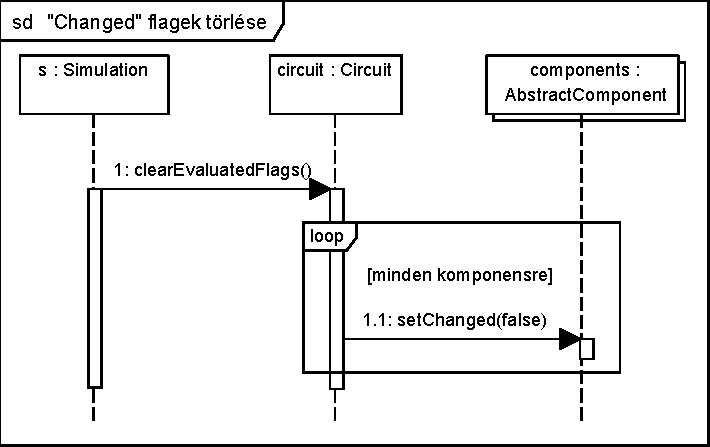
\includegraphics{chapters/chapter04/seqdiagrams/clear_changed_flags.pdf}
\caption{"Changed" flag-ek törlése}
\label{fig:clear_changed_flags}
\end{center}
\end{figure}

\begin{figure}[H]
\begin{center}
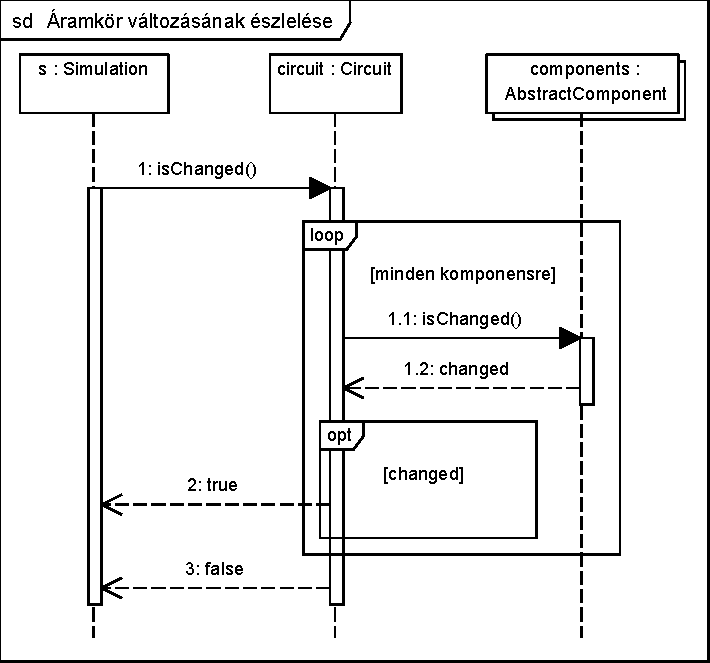
\includegraphics{chapters/chapter04/seqdiagrams/is_changed.pdf}
\caption{Áramkör változásának észlelése}
\label{fig:is_changed}
\end{center}
\end{figure}

\begin{figure}[H]
\begin{center}
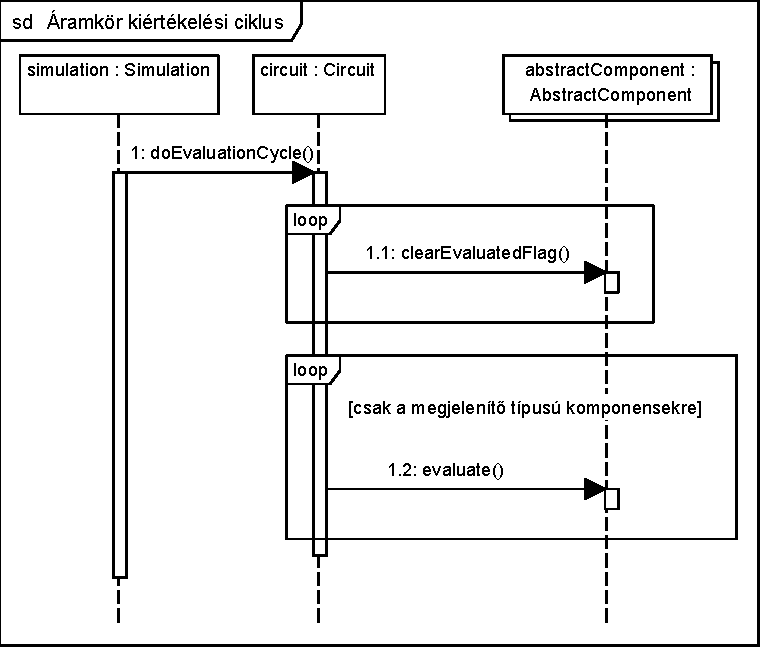
\includegraphics{chapters/chapter04/seqdiagrams/aramkor_szimulacio.pdf}
\caption{Áramkör kiértékelési ciklus}
\label{fig:circuit_sim}
\end{center}
\end{figure}

\begin{figure}[H]
\begin{center}
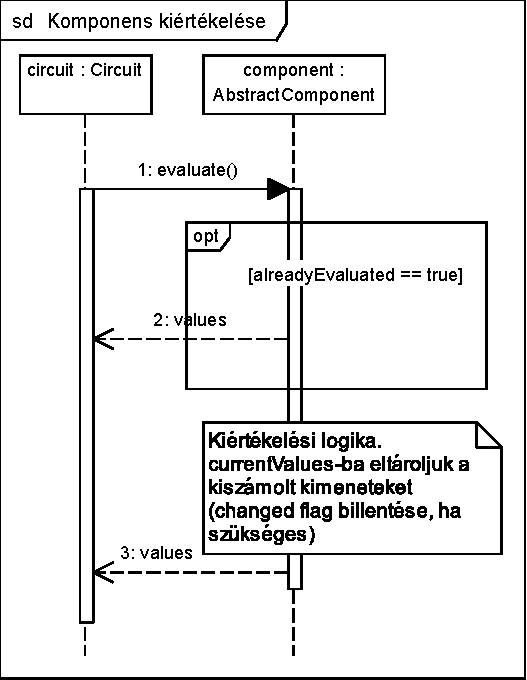
\includegraphics{chapters/chapter04/seqdiagrams/komponensek_kiertekelese.pdf}
\caption{Komponens kiértékelése}
\label{fig:component_sim}
\end{center}
\end{figure}

\begin{figure}[H]
\begin{center}
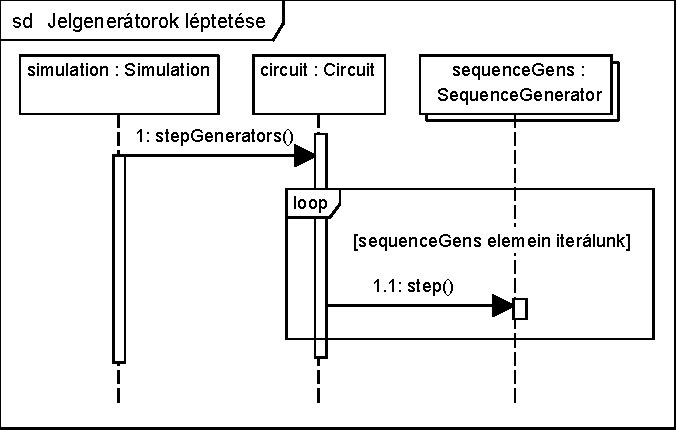
\includegraphics{chapters/chapter04/seqdiagrams/jelgeneratorok_leptetese.pdf}
\caption{Jelgenerátorok léptetése}
\label{fig:step_gens}
\end{center}
\end{figure}

\begin{figure}[H]
\begin{center}
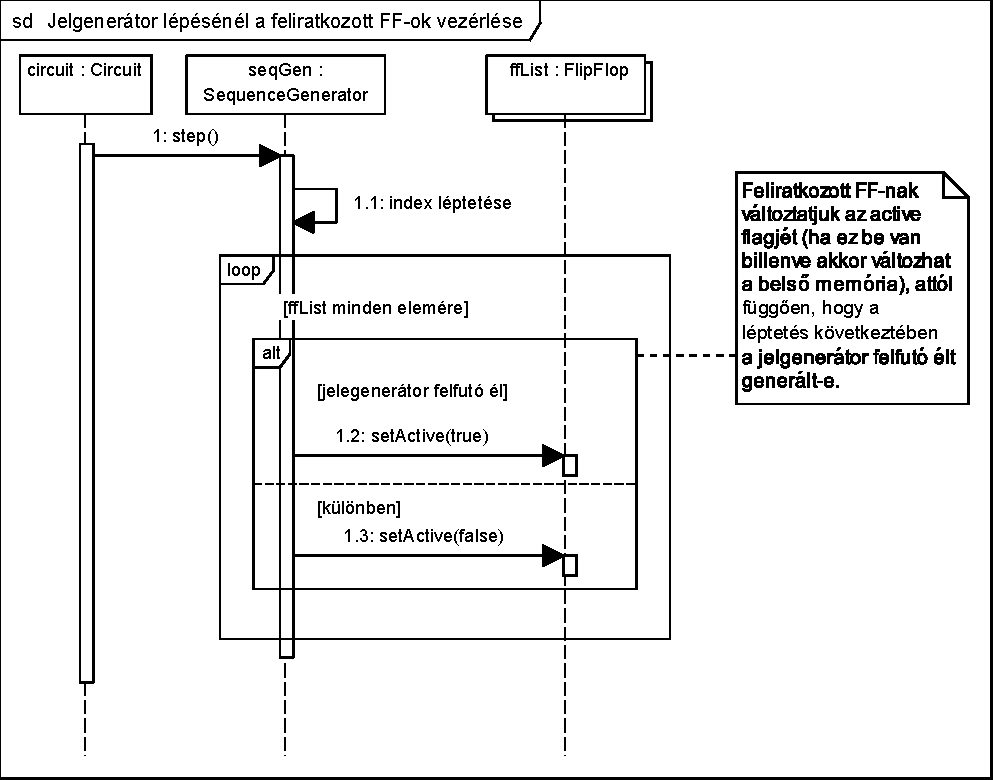
\includegraphics{chapters/chapter04/seqdiagrams/ff_on_clk.pdf}
\caption{Flip-flopok vezérlése}
\label{fig:flipflopok_vezerlese}
\end{center}
\end{figure}

\begin{figure}[H]
\begin{center}
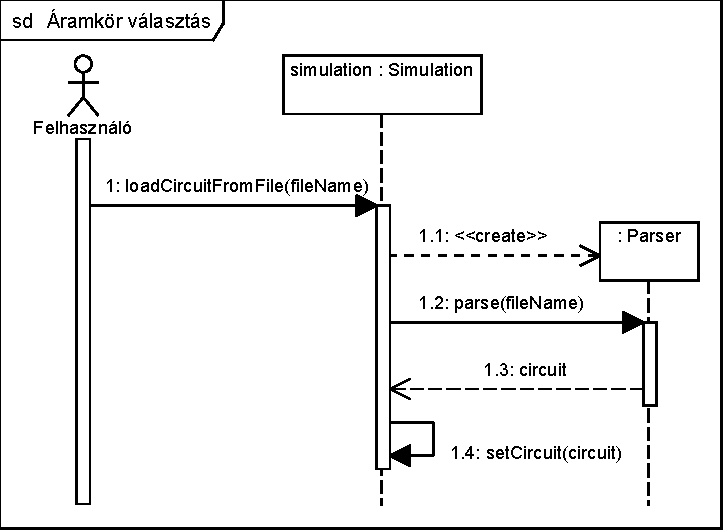
\includegraphics{chapters/chapter04/seqdiagrams/aramkor_valasztas.pdf}
\caption{Áramkör választás}
\label{fig:aramkor_valasztas}
\end{center}
\end{figure}

\begin{figure}[H]
\begin{center}
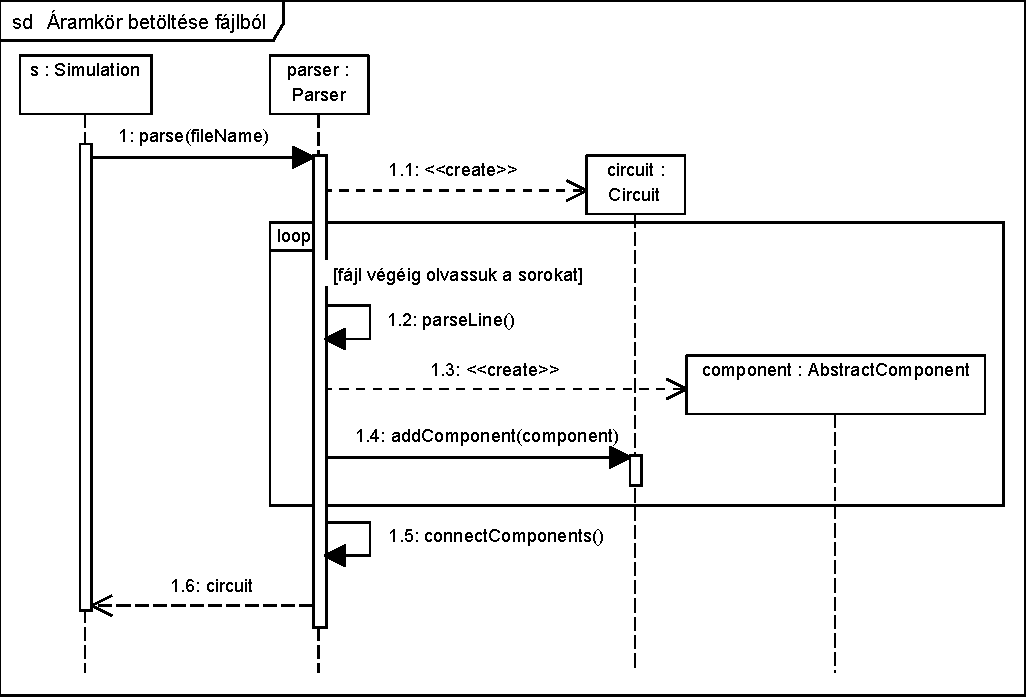
\includegraphics[width=17cm]{chapters/chapter04/seqdiagrams/aramkor_betoltes.pdf}
\caption{Áramkör betöltés fájlból}
\label{fig:aramkor_betoltes}
\end{center}
\end{figure}

\begin{figure}[H]
\begin{center}
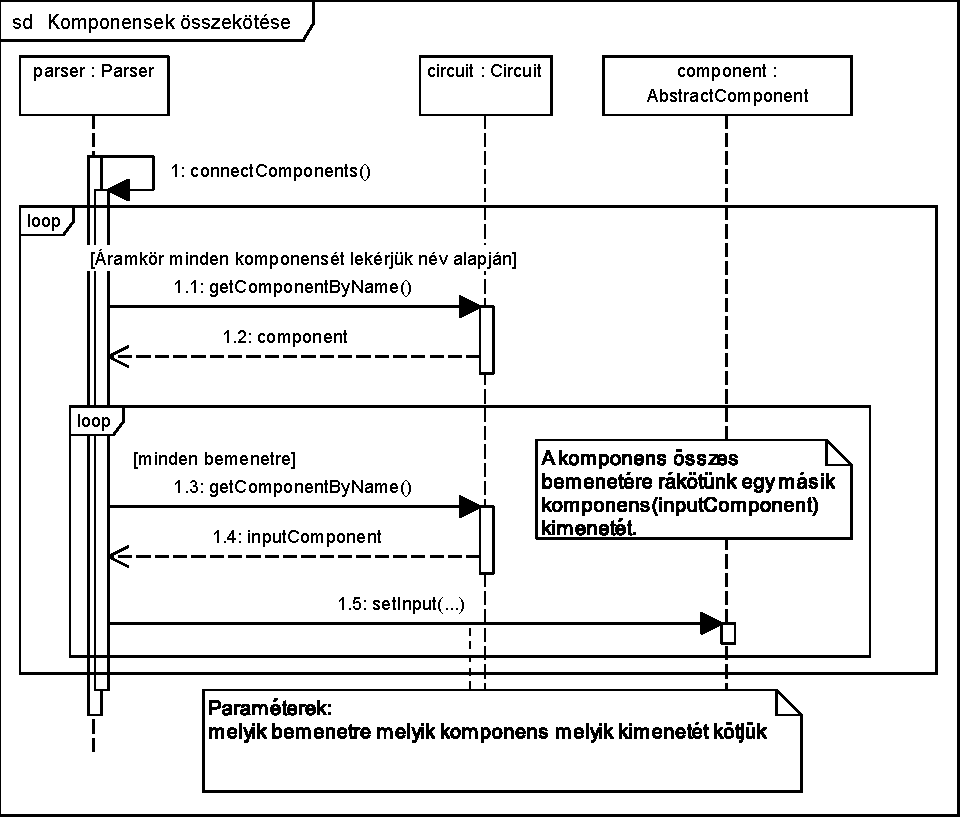
\includegraphics{chapters/chapter04/seqdiagrams/connectcomponents.pdf}
\caption{Kömponensek összekapcsolása}
\label{fig:connect_components}
\end{center}
\end{figure}

\begin{figure}[H]
\begin{center}
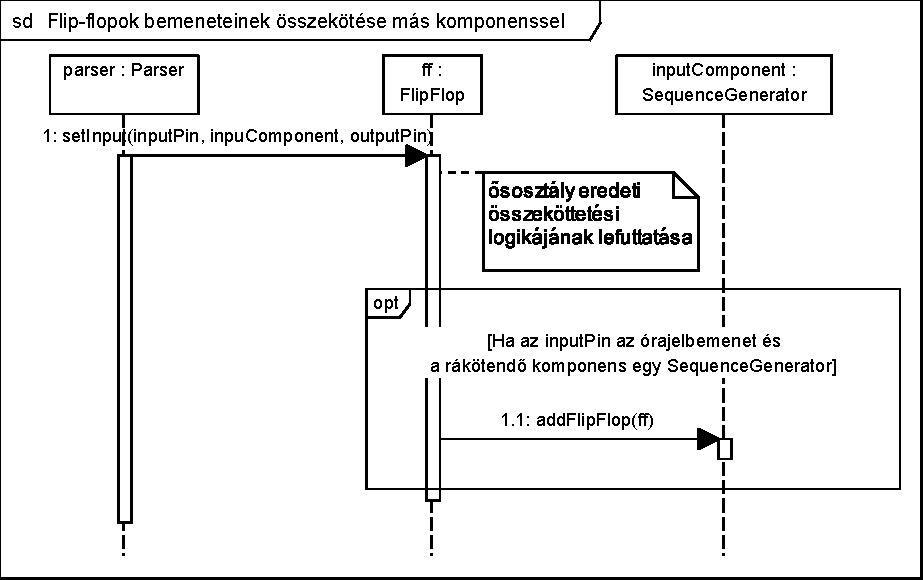
\includegraphics{chapters/chapter04/seqdiagrams/ff_bekotese.pdf}
\caption{Flip-flopok bekötése}
\label{fig:FF_connect}
\end{center}
\end{figure}

\begin{figure}[H]
\begin{center}
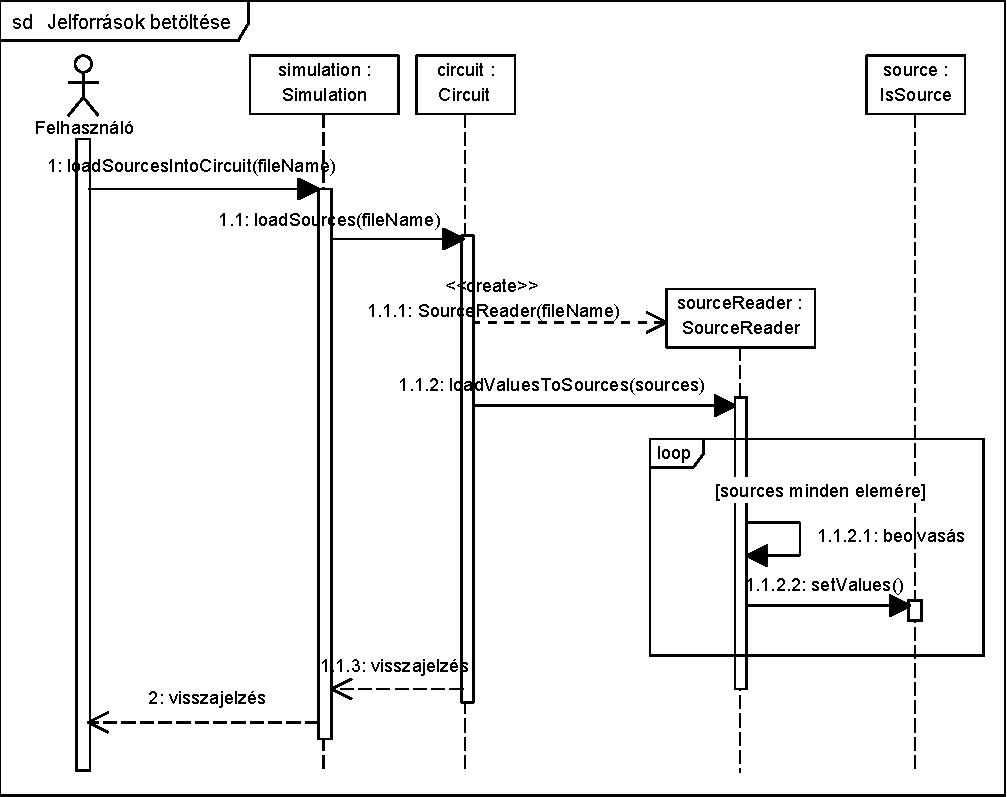
\includegraphics{chapters/chapter04/seqdiagrams/jelforrasok_betoltese.pdf}
\caption{Jelforrások betöltése}
\label{fig:jelforrasok_betoltese}
\end{center}
\end{figure}

\begin{figure}[H]
\begin{center}
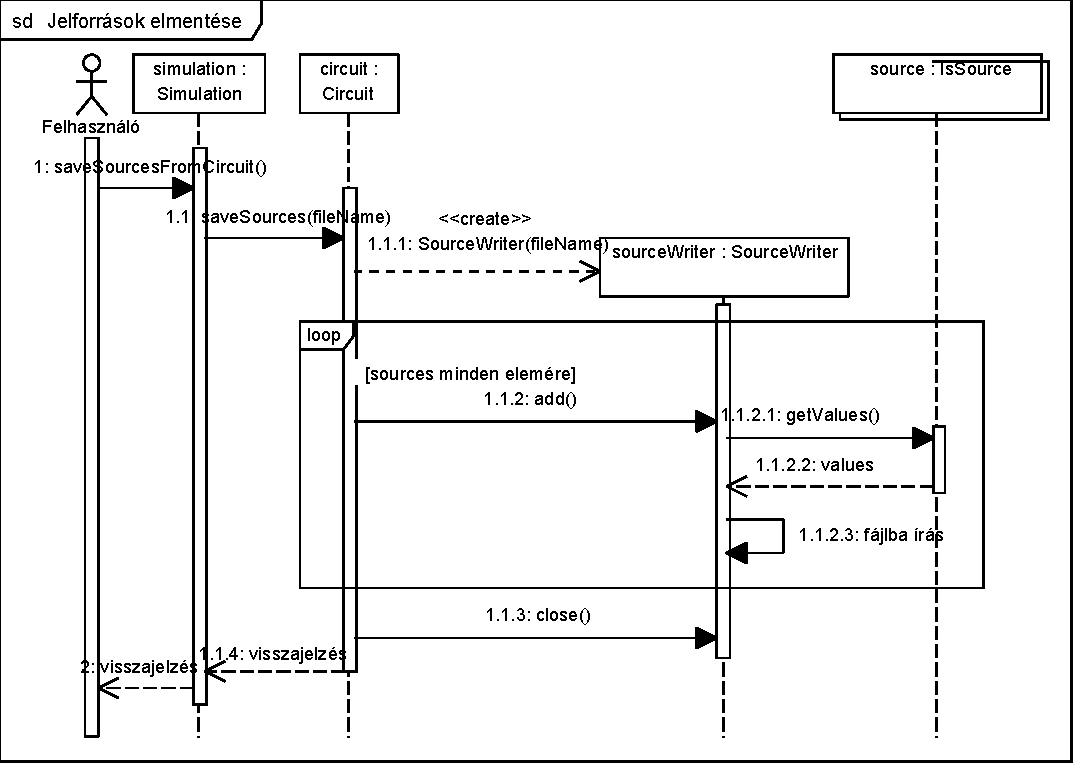
\includegraphics{chapters/chapter04/seqdiagrams/jelforrasok_mentese.pdf}
\caption{Jelforrások mentése}
\label{fig:jelforrasok_mentese}
\end{center}
\end{figure}

\begin{figure}[H]
\begin{center}
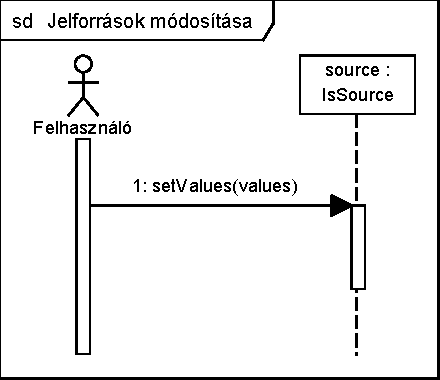
\includegraphics{chapters/chapter04/seqdiagrams/jelforrasok_modositasa.pdf}
\caption{Jelforrások módosítása}
\label{fig:jelforrasok_modositasa}
\end{center}
\end{figure}



%\begin{figure}[H]
%\begin{center}
%\includegraphics*[width = 23.5cm, angle = 90, viewport = 0 0 830 500]{chapters/chapter03/seqdiagrams/sim_running.pdf}
%\caption{Szimuláció futás közben 2. rész}
%\label{fig:sim_running2}
%\end{center}
%\end{figure}

%\begin{figure}[H]
%\begin{center}
%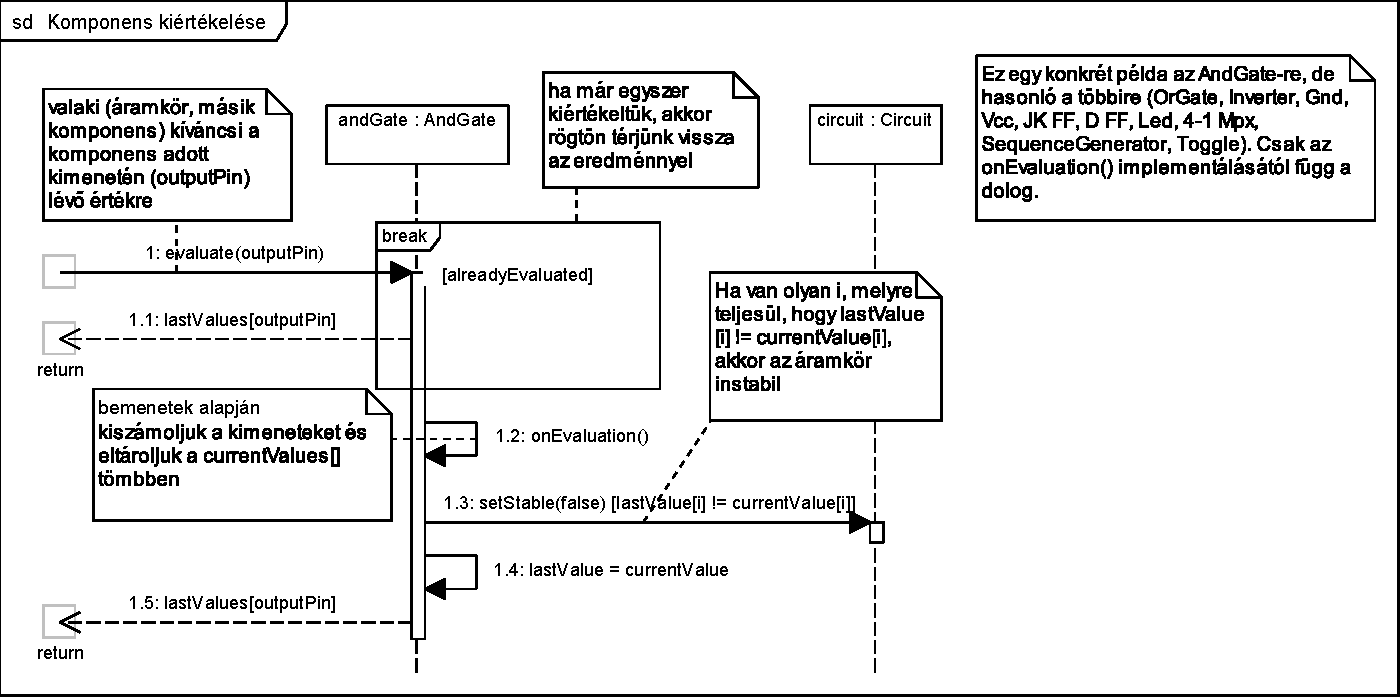
\includegraphics[angle = 90]{chapters/chapter03/seqdiagrams/sim_evaluate.pdf}
%\caption{Komponens kiértékelése}
%\label{fig:sim_evaluate}
%\end{center}
%\end{figure}
%
%\begin{figure}[H]
%\begin{center}
%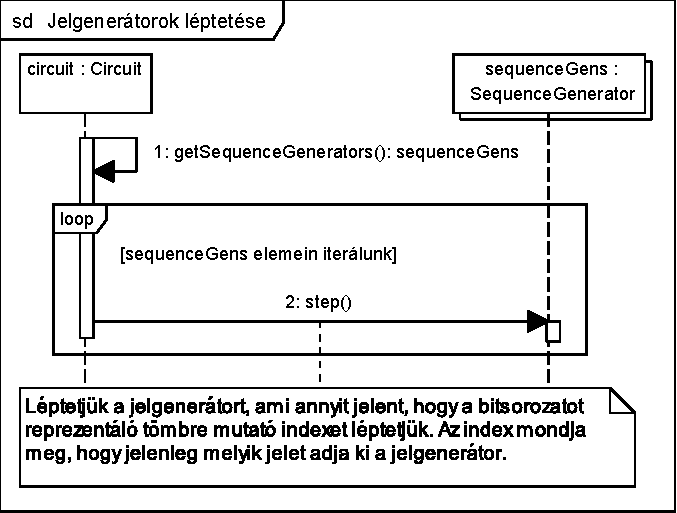
\includegraphics{chapters/chapter03/seqdiagrams/sim_stepGenerators.pdf}
%\caption{Jelgenerátorok léptetése}
%\label{fig:sim_stepGenerators}
%\end{center}
%\end{figure}
%
%\begin{figure}[H]
%\begin{center}
%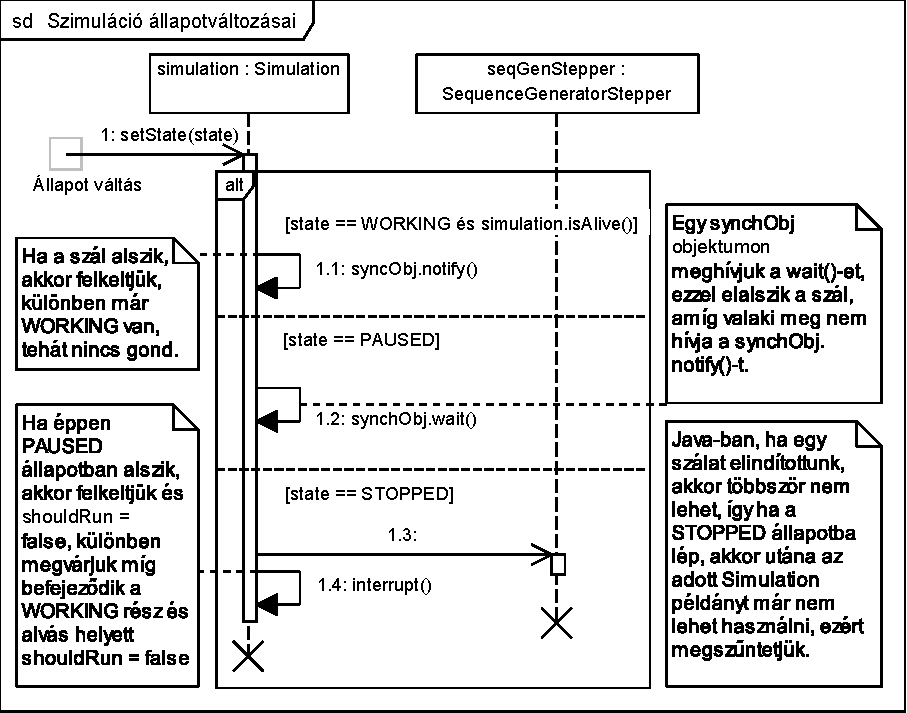
\includegraphics{chapters/chapter03/seqdiagrams/sim_allapotvaltozasai.pdf}
%\caption{Szimuláció állapotváltozásai}
%\label{fig:sim_allapotvaltozasai}
%\end{center}
%\end{figure}
%
%\begin{figure}[H]
%\begin{center}
%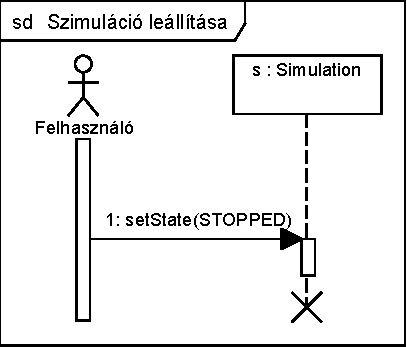
\includegraphics{chapters/chapter03/seqdiagrams/sim_stop.pdf}
%\caption{Szimuláció leállítása}
%\label{fig:sim_stop}
%\end{center}
%\end{figure}
%
%\begin{figure}[H]
%\begin{center}
%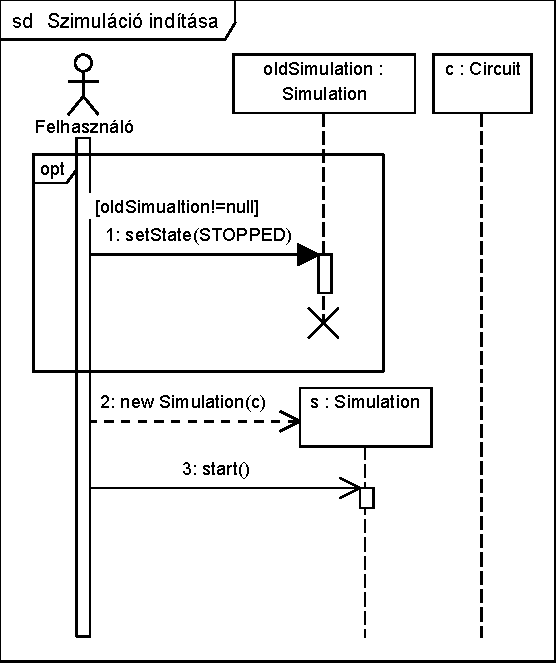
\includegraphics{chapters/chapter03/seqdiagrams/sim_start.pdf}
%\caption{Szimuláció indítása}
%\label{fig:sim_start}
%\end{center}
%\end{figure}
%
%\begin{figure}[H]
%\begin{center}
%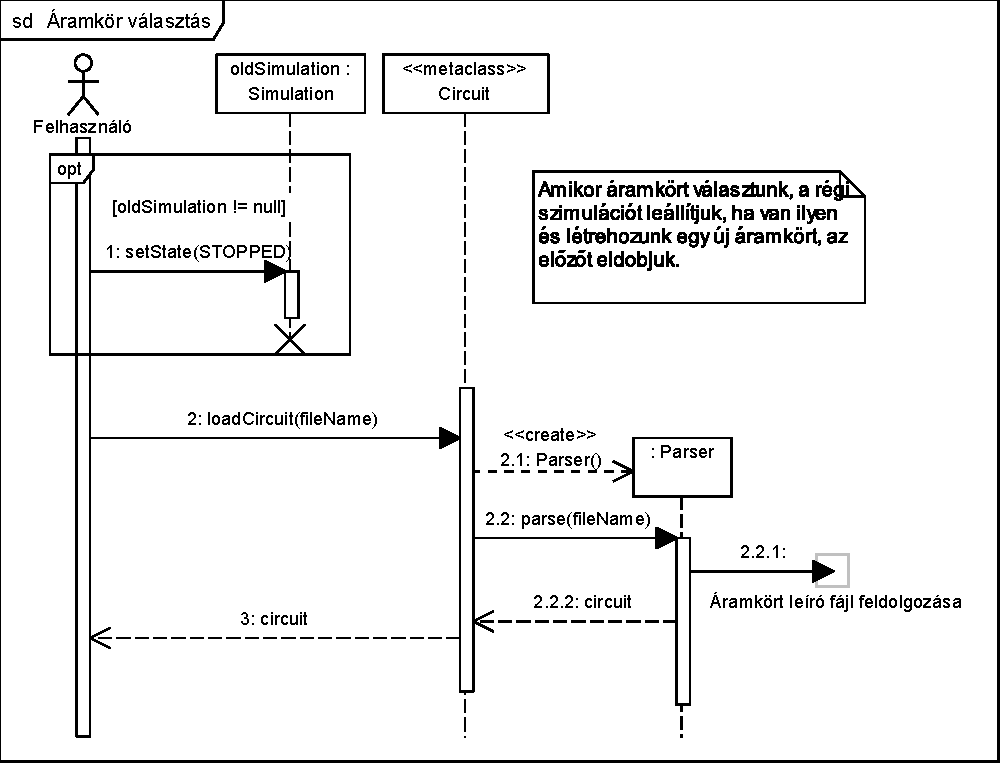
\includegraphics{chapters/chapter03/seqdiagrams/aramkor_valasztas.pdf}
%\caption{Áramkör választás}
%\label{fig:aramkor_valasztas}
%\end{center}
%\end{figure}
%
%\begin{figure}[H]
%\begin{center}
%\includegraphics*[viewport = 0 581 500 990]{chapters/chapter03/seqdiagrams/aramkor_betoltese_fajlbol.pdf}
%\caption{Áramkör betöltése fájlból 1. rész (vágva)}
%\label{fig:aramkor_betoltese_fajlbol}
%\end{center}
%\end{figure}
%
%\begin{figure}[H]
%\begin{center}
%\includegraphics*[viewport = 0 0 500 581]{chapters/chapter03/seqdiagrams/aramkor_betoltese_fajlbol.pdf}
%\caption{Áramkör betöltése fájlból 2. rész}
%\label{fig:aramkor_betoltese_fajlbol}
%\end{center}
%\end{figure}
%
%\begin{figure}[H]
%\begin{center}
%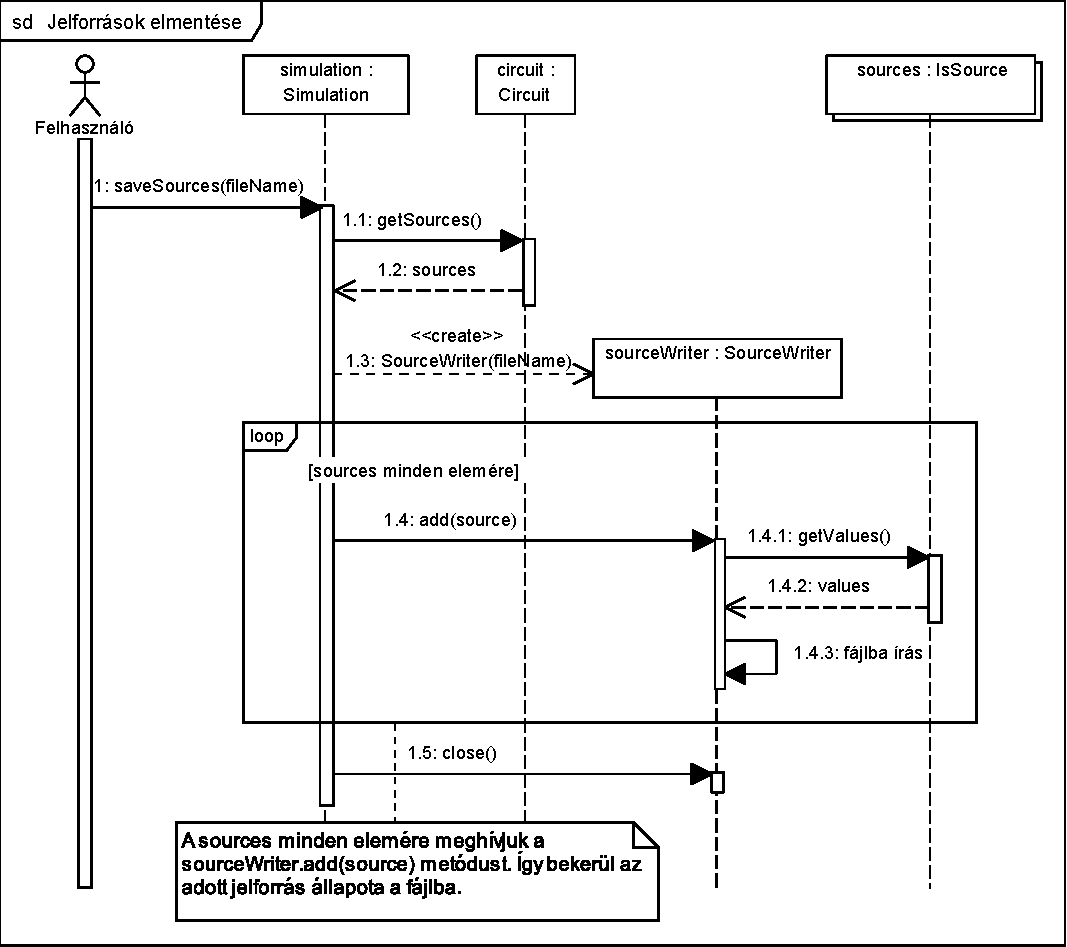
\includegraphics[width=17cm]{chapters/chapter03/seqdiagrams/jelforrasok_mentese.pdf}
%\caption{Jelforrások mentése}
%\label{fig:jelforrasok_mentese}
%\end{center}
%\end{figure}
%
%
%\begin{figure}[H]
%\begin{center}
%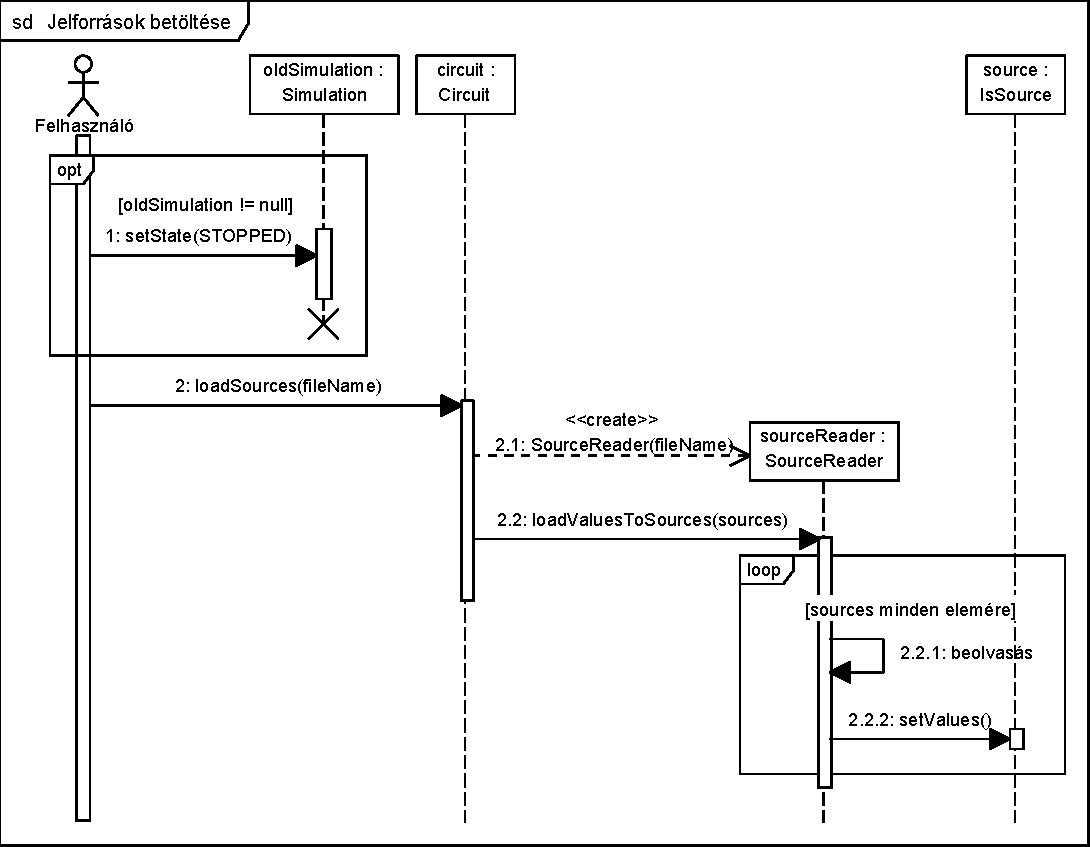
\includegraphics[angle=90]{chapters/chapter03/seqdiagrams/jelforrasok_betoltese.pdf}
%\caption{Jelforrások betöltése}
%\label{fig:jelforrasok_betoltese}
%\end{center}
%\end{figure}
%
%\begin{figure}[H]
%\begin{center}
%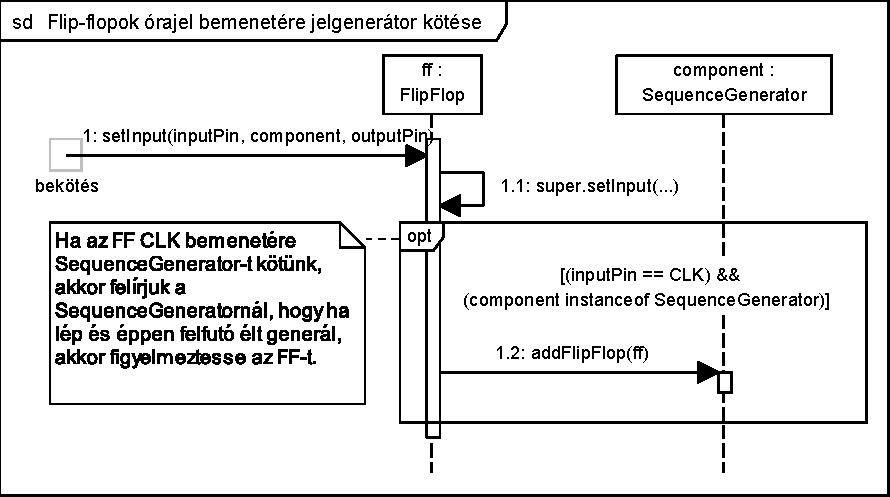
\includegraphics{chapters/chapter03/seqdiagrams/ff_bind.pdf}
%\caption{Flip-flopok órajel bemenetére jelgenerátor kötése}
%\label{fig:ff_bind}
%\end{center}
%\end{figure}
%
%\begin{figure}[H]
%\begin{center}
%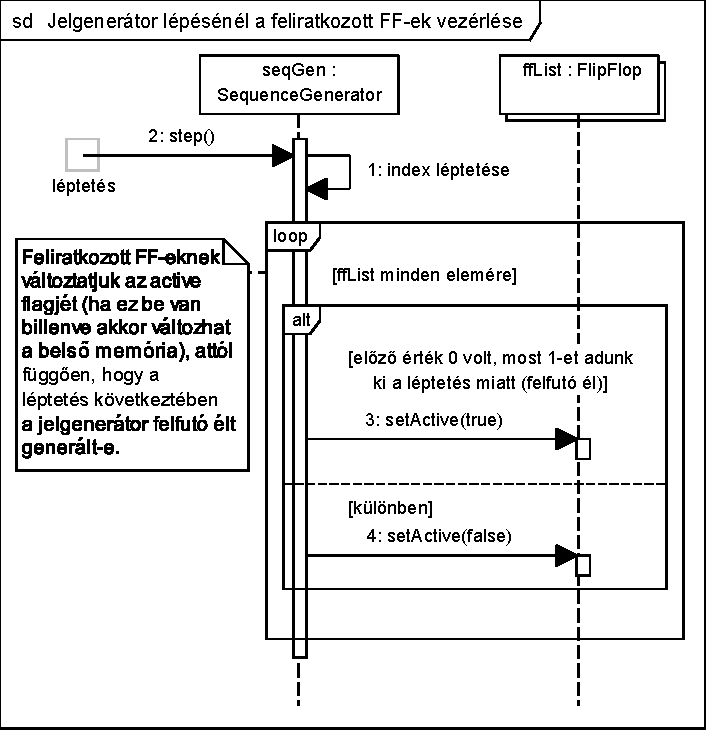
\includegraphics{chapters/chapter03/seqdiagrams/ff_vez_on_clk.pdf}
%\caption{Jelgenerátor lépésénél a feliratkozott FF-ek vezérlése}
%\label{fig:ff_vez_on_clk}
%\end{center}
%\end{figure}

\section{State-chartok}

%\begin{figure}[h]
%\begin{center}
%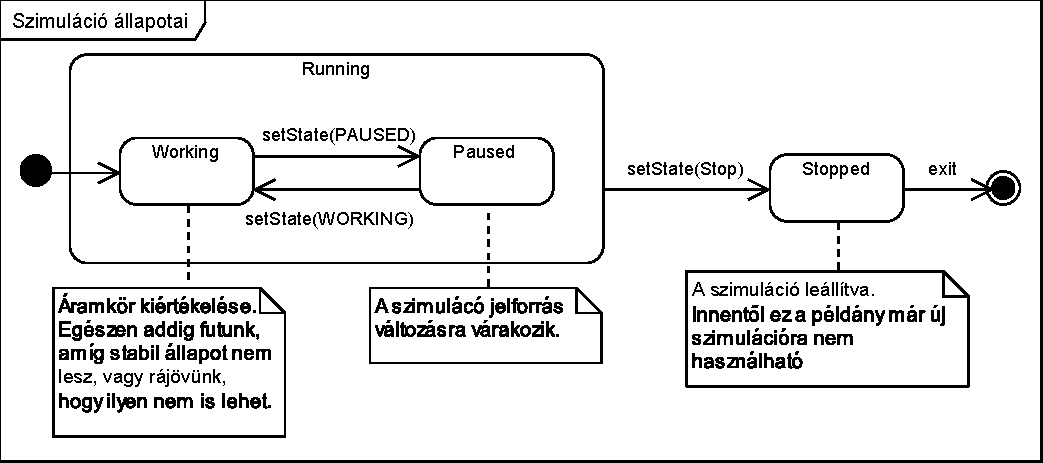
\includegraphics[width=17cm]{chapters/chapter03/seqdiagrams/sim_states.pdf}
%\caption{Szimuláció állapotai}
%\label{fig:sim_states}
%\end{center}
%\end{figure}


%% Szglab4
% ===========================================================================
%
\section{Napló}

\begin{naplo}

\bejegyzes
{2010.03.21.~18:00~} % Kezdet
{2,5 óra} % Időtartam
{Horváth\newline
Németh\newline
Tóth\newline
Oláh} % Résztvevők
{Értekezlet. Döntés: Horváth elkészíti az osztálydiagramot, Oláh a use-case leírásokat.} % Leírás

\bejegyzes
{2010.03.23.~23:00~}
{5 óra}
{Németh}
{Tevékenység: Németh implementálja a tesztelő programokat.}

\bejegyzes
{...}
{...}
{...}
{...}


\end{naplo}



%\setcounter{chapter}{4}
%% Szglab4
% ===========================================================================
%

\newcounter{enumi_saved}

\newcommand{\breaktable}{%
 \setcounter{enumi_saved}{\value{enumi}}
 \end{itemize}\end{itemize}\\
 \begin{itemize}\begin{itemize}
 \setcounter{enumi}{\value{enumi_saved}}
}

\chapter{Szkeleton tervezése}

\thispagestyle{fancy}

\section{Errata}

Az előző fejezetben leírtak egy apró részletben megváltoztak. Az elemeket már nem közvetlenül kötjük össze, hanem \textit{vezeték}ek segítségével, melyeket egymással \textit{csomópont}okkal lehet összekötni, ha szükséges. Így javítottuk a láthatósággal kapcsolatosan felmerült problémákat, ehhez fel kellett venni 2 új osztályt (Wire, Node), illetve az AbstractComponent módosítani, ezekhez tartozó objektum és osztályleírások alább olvashatóak, valamint mellékeltük a módosított statikus osztálydiagramot is. (Egy-két egyéb objektumleírás is módosult, de csak azért mert a kiértékelés logikája változott -- nem hátulról megyünk, hanem az összes kiértékeli magát, ez nem szükséges a jelen fejezethez, hiszen magától értetődő apróbb átfogalmazásokról van szó)

\subsection{Objektumleírás: \bf Wire}
Vezeték, mely az áramköri komponensek ki és bemeneteit köti össze. Egy vezeték egy darab kimenetet és egy darab bemenetet köt össze. A rajta lévő értéket le lehet tőle kérdezni, illetve be lehet azt állítani.

\subsection{Objektumleírás: \bf Node}
Csomópont, mely a bemenetén lévő értéket a kimeneteire adja. Segítségével lehet egy vezetéket ,,szétágaztatni''.

\subsection{Osztályleírás: \bf AbstractComponent}
Absztrakt osztály.
\begin{itemize}
\item Felelősség\\
Egy komponens absztrakt megvalósítása, ebből származik az összes többi  komponens. A közös logikát valósítja meg. A gyakran használt feladatokra ad alapértelmezett implementációt (pl. vezetékek bekötése). Tudja magáról, hogy a legutóbbi két kiértékelés között változtak-e a kimenetei.
\item Ősosztályok: (nincs)
\item Interfészek: (nincs)
\item Attribútumok $\ $
\begin{itemize}
	\item \texttt{protected Wire[] inputs}: Bemeneteire kötött vezetékek.
	\item \texttt{protected Wire[] outputs}: Kimeneteire kötött vezetékek.
\end{itemize}
\item Metódusok$\ $
\begin{itemize}
	\item \texttt{addTo(Circuit c)}: Meghívja az áramkör \texttt{add(AbstractComponent ac)} metódusát.
	\item \texttt{void evaluate()}: Komponens kimenetein lévő értékek kiszámolása a bemenetek alapján.
	\item \texttt{boolean isChanged()}: Visszaadja, hogy a legutóbbi két kiértékelés között változtak-e a kimenetek.
	\item \texttt{void setInput(int inputPin, Wire wire)}: Az adott bemeneti lábára rákötjük a megadott vezetéket.
	\item \texttt{void setOutput(int outputPin, Wire wire)}: Az adott kimeneti lábára rákötjük a megadott vezetéket.
\end{itemize}
\end{itemize}

\subsection{Osztályleírás: \bf Node}
\begin{itemize}
\item Felelősség\\
Csomópont, mely a bemenetén lévő értéket a kimeneteire adja. Segítségével lehet egy vezetéket ,,szétágaztatni''.
\item Ősosztályok:\ AbstractComponent.
\item Interfészek: (nincs)
\item Attribútumok $\ $
\begin{itemize}
\item (nincs)
\end{itemize}
\item Metódusok$\ $
\begin{itemize}
\item (nincs)
\end{itemize}
\end{itemize}

\subsection{Osztályleírás: \bf Wire}
\begin{itemize}
\item Felelősség\\
Vezeték, mely az áramköri komponensek ki és bemeneteit köti össze. Egy vezeték egy darab kimenetet és egy darab bemenetet köt össze. A rajta lévő értéket le lehet tőle kérdezni, illetve be lehet azt állítani.
\item Ősosztályok:\ AbstractComponent.
\item Interfészek: (nincs)
\item Attribútumok $\ $
\begin{itemize}
	\item \texttt{private Value value}: Vezetéken lévő érték
\end{itemize}
\item Metódusok$\ $
\begin{itemize}
	\item \texttt{Value getValue()}: Visszaadja a vezetéken lévő értéket.
	\item \texttt{void setValue(Value v)}: Beállítja a vezetéken lévő értéket.
\end{itemize}
\end{itemize}

\subsection{Statikus struktúra diagramok}

\begin{figure}[H]
\begin{center}
\includegraphics*[angle=90, width=17cm, viewport = 25 30 705 565]{chapters/chapter04/classdiagram/class.pdf}
\caption{Statikus struktúra nézet}
\label{fig:class_diagram}
\end{center}
\end{figure}

\section{A szkeleton modell valóságos use-case-ei}

\subsection{Use-case diagram}

\begin{figure}[h]
\begin{center}
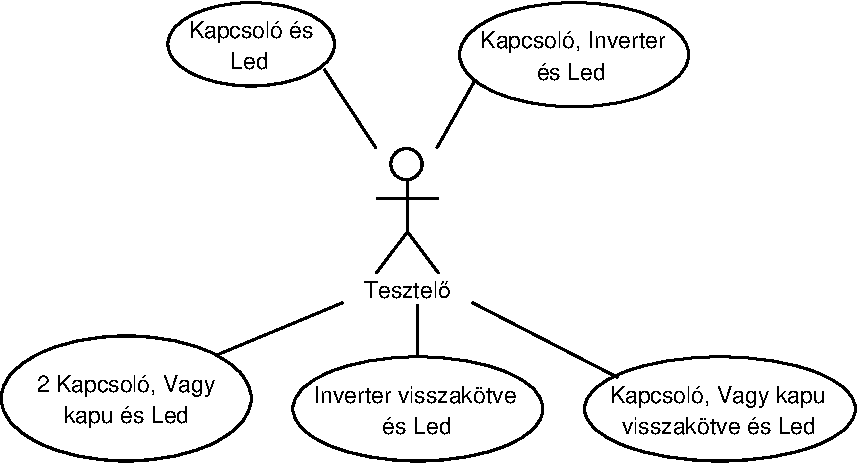
\includegraphics[width=10cm]{chapters/chapter05/imgs/usecase.pdf}
\caption{A szkeleton modell valóságos use-case-ei}
\label{fig:SzkeletonUseCase}
\end{center}
\end{figure}

\subsection{Use-case leírások}

Lenti use-caseknél, ahol valamilyen információ szerint dönteni kell, vagy csak szükségünk van a skeleton jellegéből adódó hiányzó információkra, azt a felhasználótól kérjük be. Ahhoz, hogy a szekvenciadiagramokon lévő szekvenciákat kapjunk, a javasolt értéket kell beírnia a tesztelőnek.\\

Nem akartuk, hogy az áramkör inicializálása minden use-casenél ott legyen, ezzel elfedve a lényegi részeket, ezért ezt egy külön use-case-ben bemutatjuk, a többinél csak jelezzük, hogy ott is van ilyen lépés. A tesztelő, majd egy adott tesztesetnél választhat, hogy kíváncsi-e az inicializálásra vagy sem.\\

Kapcsolók állítása nincs benne egyik use-caseben sem, azért mert ez ténylegesen majd a szimuláción kívül fog történni, de a kapcsolók bekérik az állapotukat a felhasználótól, így a szimuláció teszteléséhez ez nem is szükséges.

\usecase
{Áramkör inicializálása}
{Ez a usecase egy áramkör és a hozzá tartozó szimuláció inicializálását mutatja be, hogyan jönnek létre a komponensek és a közöttük lévő összeköttetések. Jelen példa egy Kapcsoló és egy Led összeköttetését prezentálja.}
{Tesztelő}
{\vspace{-15pt}
\begin{itemize}
\setlength{\itemsep}{0cm}%
\setlength{\parskip}{0cm}%
\item szimuláció létrehozása
\item áramkör létrehozása
\item áramkör inicializálása
\begin{itemize}
\setlength{\itemsep}{0cm}%
\setlength{\parskip}{0cm}%
	\item kapcsoló létrehozása
	\item vezeték létrehozása
	\item kapcsoló kimenetére vezeték kötése
	\item led létrehozása
	\item led bemenetére vezeték kötése
	\item kapcsoló áramkörbe regisztrálása
	\item led áramkörbe regisztrálása
\end{itemize}
\item áramkör beregisztrálása a szimulációba
\end{itemize}
\vspace{-15pt}}

\newpage

\usecase
{Kapcsoló és Led}
{Ez a usecase egy olyan áramkör tesztelését mutatja be, amely egy kapcsolóból és rá kötött ledből áll.\newline
\begin{center}
\vspace{-15pt}
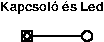
\includegraphics[scale=1.5]{dw/circuit_test1.pdf}
\vspace{-10pt}
\end{center}
}
{Tesztelő}
{\vspace{-15pt}
\begin{itemize}
\setlength{\itemsep}{0cm}%
\setlength{\parskip}{0cm}%
\item Áramkör és komponensek létrehozása
%\begin{itemize}
%\setlength{\itemsep}{0cm}%
%\setlength{\parskip}{0cm}%
%\item áramkör létrehozása
%\item áramkör beregisztrálása a szimulációba
%\item vezeték létrehozása
%\item kapcsoló létrehozása
%\item kapcsoló kimenetére vezeték kötése
%\item led létrehozása
%\item led bemenetére vezeték kötése
%\item kapcsoló áramkörbe regisztrálása
%\item led áramkörbe regisztrálása
%\end{itemize}
\item szimuláció indítása
\begin{itemize}
\setlength{\itemsep}{0cm}%
\setlength{\parskip}{0cm}%
\item hálózat kiértékelés indítása
\begin{itemize}
\setlength{\itemsep}{0cm}%
\setlength{\parskip}{0cm}%
	\item kapcsoló kiértékelése
	\begin{itemize}
	\setlength{\itemsep}{0cm}%
	\setlength{\parskip}{0cm}%
		\item kapcsoló állapotának lekérdezése (\textbf{megkérdezi a tesztelőt}, javasolt: 1)
		\item kapcsoló értékének kiadása a vezetékre
	\end{itemize}
	\item led kiértékelése
	\begin{itemize}
	\setlength{\itemsep}{0cm}%
	\setlength{\parskip}{0cm}%
		\item led bemenetének lekérdezése (\textbf{megkérdezi a tesztelőt}, javasolt: 1)
	\end{itemize}
\end{itemize}
\item áramkör változásának vizsgálata
\begin{itemize}
\setlength{\itemsep}{0cm}%
\setlength{\parskip}{0cm}%
	\item kapcsoló változásának vizsgálata (\textbf{megkérdezi a tesztelőt}, javasolt: 1)
	\item led változásának vizsgálata (\textit{idáig nem kéne eljutni, ha fent jót válaszolt a tesztelő})
\end{itemize}
\item áramkör változott, ezért új ciklus
\item hálózat kiértékelés indítása
\begin{itemize}
\setlength{\itemsep}{0cm}%
\setlength{\parskip}{0cm}%
	\item \textit{ugyanazon lépések történnek mint az előző kiértékelésnél, és ugyanazon válaszokat javasolt adni.}
\end{itemize}
\item áramkör változásának vizsgálata
\begin{itemize}
\setlength{\itemsep}{0cm}%
\setlength{\parskip}{0cm}%
	\item kapcsoló változásának vizsgálata (\textbf{megkérdezi a tesztelőt}, javasolt: 0)
	\item led változásának vizsgálata (\textbf{megkérdezi a tesztelőt}, javasolt: 0)
\end{itemize}
\item áramkör nem változott, stabil állapot
\item FF-okat véglegesítjük (nem történik semmi, mert nincs FF)
\item jelgenerátorokat léptetjük (nem történik semmi, mert nincs jelgenerátor)
\item szimuláció vége
\end{itemize}
\end{itemize}
\vspace{-15pt}}

\newpage

\usecase
{Kapcsoló, Inverter és Led}
{Ez a usecase egy olyan áramkör tesztelését mutatja be, amely egy kapcsolóból egy rá kötött inverterből és egy arra kötött ledből áll.\newline
\begin{center}
\vspace{-15pt}
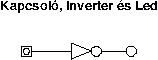
\includegraphics[scale=1.5]{dw/circuit_test2.pdf}
\vspace{-10pt}
\end{center}}
{Tesztelő}
{\vspace{-15pt}
\begin{itemize}
\setlength{\itemsep}{0cm}%
\setlength{\parskip}{0cm}%
\setlength{\itemindent}{-10pt}%
\item Áramkör és komponensek létrehozása
%\begin{itemize}
%\setlength{\itemsep}{0cm}%
%\setlength{\parskip}{0cm}%
%\item áramkör létrehozása
%\item áramkör beregisztrálása a szimulációba
%\item vezeték létrehozása a kapcsoló és az inverter összekötéséhez
%\item kapcsoló létrehozása
%\item kapcsoló kimenetére vezeték kötése
%\item inverter létrehozása
%\item inverter bemenetére vezeték kötése
%\item vezeték lérehozása az inverter és a led összekötéséhez
%\item inverter kimenetére vezeték kötése
%\item led létrehozása
%\item led bemenetére vezeték kötése
%\item kapcsoló áramkörhöz adása
%\item led áramkörhöz adása
%\item inverter áramkörhöz adása
%\end{itemize}
\item szimuláció indítása
\begin{itemize}
\setlength{\itemsep}{0cm}%
\setlength{\parskip}{0cm}%
\setlength{\itemindent}{-25pt}%
\item hálózat kiértékelés indítása
\begin{itemize}
\setlength{\itemsep}{0cm}%
\setlength{\parskip}{0cm}%
\setlength{\itemindent}{-25pt}%
	\item kapcsoló kiértékelése
	\begin{itemize}
	\setlength{\itemsep}{0cm}%
	\setlength{\parskip}{0cm}%
	\setlength{\itemindent}{-35pt}%
		\item kapcsoló állapotának lekérdezése (\textbf{megkérdezi a tesztelőt}, javasolt: 1)
		\item kapcsoló értékének kiadása a vezetékre
	\end{itemize}
	\item inverter kiértékelése
	\begin{itemize}
	\setlength{\itemsep}{0cm}%
	\setlength{\parskip}{0cm}%
	\setlength{\itemindent}{-35pt}%
		\item bemenet lekérdezése (\textbf{megkérdezi a tesztelőt}, javasolt: 1)
		\item kimenet kiadása a vezetékre (\textbf{megkérdezi a tesztelőt}, javasolt: 0)
	\end{itemize}\item led kiértékelése
	\begin{itemize}
	\setlength{\itemsep}{0cm}%
	\setlength{\parskip}{0cm}%
	\setlength{\itemindent}{-35pt}%
		\item led bemenetének lekérdezése (\textbf{megkérdezi a tesztelőt}, javasolt: 0)
	\end{itemize}
\end{itemize}
\item áramkör változásának vizsgálata
\begin{itemize}
\setlength{\itemsep}{0cm}%
\setlength{\parskip}{0cm}%
\setlength{\itemindent}{-25pt}%
	\item kapcsoló változásának vizsgálata (\textbf{megkérdezi a tesztelőt}, javasolt: 1)
	\item inverter változásának vizsgálata (\textit{idáig nem kéne eljutni, ha fent jót válaszolt a tesztelő})
	\item led változásának vizsgálata (\textit{idáig nem kéne eljutni, ha fent jót válaszolt a tesztelő})
\end{itemize}
\item áramkör változott, ezért új ciklus
\item hálózat kiértékelés indítása
\begin{itemize}
\setlength{\itemsep}{0cm}%
\setlength{\parskip}{0cm}%
\setlength{\itemindent}{-25pt}%
	\item \textit{ugyanazon lépések történnek mint az előző kiértékelésnél, és ugyanazon válaszokat javasolt adni.}
\end{itemize}
\item áramkör változásának vizsgálata
\begin{itemize}
\setlength{\itemsep}{0cm}%
\setlength{\parskip}{0cm}%
\setlength{\itemindent}{-25pt}%
	\item kapcsoló változásának vizsgálata (\textbf{megkérdezi a tesztelőt}, javasolt: 0)
	\item inverter változásának vizsgálata (\textbf{megkérdezi a tesztelőt}, javasolt: 0)
	\item led változásának vizsgálata (\textbf{megkérdezi a tesztelőt}, javasolt: 0)
\end{itemize}
\item áramkör nem változott, stabil állapot
\item FF-okat véglegesítjük (nem történik semmi, mert nincs FF)
\item jelgenerátorokat léptetjük (nem történik semmi, mert nincs jelgenerátor)
\item szimuláció vége
\end{itemize}
\end{itemize}
\vspace{-15pt}}

\newpage
\vspace*{-30pt}

	\begin{longtable}{| l | p{12cm} |}
	\hline
	\textbf{Use-case neve}   & {2 Kapcsoló, Vagy kapu és Led} \tabularnewline
	\hline\hline
	Rövid leírás    & {Ez a usecase egy olyan áramkör tesztelését mutatja be, amely egy vagy kapura kötött két kapcsolóból és a vagy kapu kimenetére kötött ledből áll.\newline
\begin{center}
\vspace{-15pt}
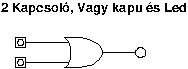
\includegraphics[scale=1.5]{dw/circuit_test3.pdf}
\vspace{-10pt}
\end{center}} \tabularnewline
	\hline
	Aktorok         & {Tesztelő} \tabularnewline
	\hline
	Forgatókönyv    &  \vspace{-15pt}
\begin{itemize}
\setlength{\itemsep}{0cm}%
\setlength{\parskip}{0cm}%
\setlength{\itemindent}{-15pt}%
\item Áramkör és komponensek létrehozása
\item Szimuláció indítása
\begin{itemize}
\setlength{\itemsep}{0cm}%
\setlength{\parskip}{0cm}%
\setlength{\itemindent}{-35pt}%
\item hálózat kiértékelés indítása
\begin{itemize}
\setlength{\itemsep}{0cm}%
\setlength{\parskip}{0cm}%
\setlength{\itemindent}{-50pt}%
	\item 1. kapcsoló kiértékelése
	\begin{itemize}
	\setlength{\itemsep}{0cm}%
	\setlength{\parskip}{0cm}%
	\setlength{\itemindent}{-60pt}%
		\item kapcsoló állapotának lekérdezése (\textbf{megkérdezi a tesztelőt}, javasolt: 0)
		\item kapcsoló értékének kiadása a vezetékre
	\end{itemize}
	\item 2. kapcsoló kiértékelése
	\begin{itemize}
	\setlength{\itemsep}{0cm}%
	\setlength{\parskip}{0cm}%
	\setlength{\itemindent}{-60pt}%
		\item kapcsoló állapotának lekérdezése (\textbf{megkérdezi a tesztelőt}, javasolt: 1)
		\item kapcsoló értékének kiadása a vezetékre
	\end{itemize}
	\item VAGY kapu kiértékelése
	\begin{itemize}
	\setlength{\itemsep}{0cm}%
	\setlength{\parskip}{0cm}%
	\setlength{\itemindent}{-60pt}%
		\item kapu egyik bemenetének lekérdezése (\textbf{megkérdezi a tesztelőt}, javasolt: 0)
		\item kapu másik bemenetének lekérdezése (\textbf{megkérdezi a tesztelőt}, javasolt: 1)
		\item kapu értékének kiadása a vezetékre (\textbf{megkérdezi a tesztelőt}, javasolt: 1)
	\end{itemize}
	\item led kiértékelése
	\begin{itemize}
	\setlength{\itemsep}{0cm}%
	\setlength{\parskip}{0cm}%
	\setlength{\itemindent}{-60pt}%
		\item led bemenetének lekérdezése (\textbf{megkérdezi a tesztelőt}, javasolt: 1)
	\end{itemize}
\end{itemize}
\item áramkör változásának vizsgálata
\begin{itemize}
\setlength{\itemsep}{0cm}%
\setlength{\parskip}{0cm}%
\setlength{\itemindent}{-50pt}%
	\item 1. kapcsoló változásának vizsgálata (\textbf{megkérdezi a tesztelőt}, javasolt: 0)
	\item 2. kapcsoló változásának vizsgálata (\textbf{megkérdezi a tesztelőt}, javasolt: 1)
	\item kapu változásának vizsgálata (\textit{idáig nem kéne eljutni, ha fent jót válaszolt a tesztelő})
	\item led változásának vizsgálata (\textit{idáig nem kéne eljutni, ha fent jót válaszolt a tesztelő})
\end{itemize}
\item áramkör változott, ezért új ciklus
\item hálózat kiértékelés indítása
\begin{itemize}
\setlength{\itemsep}{0cm}%
\setlength{\parskip}{0cm}%
\setlength{\itemindent}{-50pt}%
	\item \textit{ugyanazon lépések történnek mint az előző kiértékelésnél, és ugyanazon válaszokat javasolt adni.}
\end{itemize}
\item áramkör változásának vizsgálata
\begin{itemize}
\setlength{\itemsep}{0cm}%
\setlength{\parskip}{0cm}%
\setlength{\itemindent}{-50pt}%
	\item 1. kapcsoló változásának vizsgálata (\textbf{megkérdezi a tesztelőt}, javasolt: 0)
	\item 2. kapcsoló változásának vizsgálata (\textbf{megkérdezi a tesztelőt}, javasolt: 0)
	\item kapu változásának vizsgálata (\textbf{megkérdezi a tesztelőt}, javasolt: 0)
	\item led változásának vizsgálata (\textbf{megkérdezi a tesztelőt}, javasolt: 0)
\end{itemize}
\item áramkör nem változott, stabil állapot
\item FF-okat véglegesítjük (nem történik semmi, mert nincs FF)
\item jelgenerátorokat léptetjük (nem történik semmi, mert nincs jelgenerátor)
\item stacionárius állapot, szimuláció vége
\end{itemize}
\end{itemize}
\vspace{-15pt}\tabularnewline
	\hline
	\end{longtable}

\newpage

\usecase
{Inverter visszakötve és Led}
{Ez a usecase egy olyan áramkör tesztelését mutatja be, amely egy inverterből, amelynek kimenete egy ledbe illetve saját bemenetére van kötve. Oszcillálni fog, ezért a szimuláció rövid időn belül leáll.
\newline
\begin{center}
\vspace{-15pt}
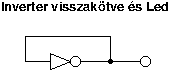
\includegraphics[scale=1.5]{dw/circuit_test4.pdf}
\vspace{-10pt}
\end{center}}
{Tesztelő}
{\vspace{-10pt}
\begin{itemize}
\setlength{\itemsep}{0cm}%
\setlength{\parskip}{0cm}%
\setlength{\itemindent}{-15pt}%
\item Áramkör és komponensek létrehozása
\item szimuláció indítása
\begin{itemize}
\setlength{\itemsep}{0cm}%
\setlength{\parskip}{0cm}%
\setlength{\itemindent}{-35pt}%
\item hálózat kiértékelés indítása
\begin{itemize}
\setlength{\itemsep}{0cm}%
\setlength{\parskip}{0cm}%
\setlength{\itemindent}{-50pt}%
	\item inverter kiértékelése
	\begin{itemize}
	\setlength{\itemsep}{0cm}%
	\setlength{\parskip}{0cm}%
	\setlength{\itemindent}{-65pt}%
		\item inverter bemenetének lekérdezése (\textbf{megkérdezi a tesztelőt}, javasolt: 0)
		\item inv. értékének kiadása a vezetékre (\textbf{megkérdezi a tesztelőt}, javasolt: 1)
	\end{itemize}
	\item node kiértékelése
	\begin{itemize}
	\setlength{\itemsep}{0cm}%
	\setlength{\parskip}{0cm}%
	\setlength{\itemindent}{-65pt}%
		\item node bemenetének lekérdezése (\textbf{megkérdezi a tesztelőt}, javasolt: 1)
		\item node értékének kiadása a vezetékekre (\textbf{megkérdezi a tesztelőt}, javasolt: mindkettőre 1)
	\end{itemize}
	\item led kiértékelése
	\begin{itemize}
	\setlength{\itemsep}{0cm}%
	\setlength{\parskip}{0cm}%
	\setlength{\itemindent}{-65pt}%
		\item led bemenetének lekérdezése (\textbf{megkérdezi a tesztelőt}, javasolt: 1)
	\end{itemize}
\end{itemize}
\item áramkör változásának vizsgálata
\begin{itemize}
\setlength{\itemsep}{0cm}%
\setlength{\parskip}{0cm}%
\setlength{\itemindent}{-50pt}%
	\item inverter változásának vizsgálata (\textbf{megkérdezi a tesztelőt}, javasolt: 1)
	\item led változásának vizsgálata (\textit{idáig nem kéne eljutni, ha fent jót válaszolt a tesztelő})
\end{itemize}
\item áramkör változott, ezért új ciklus
\item hálózat kiértékelés indítása
\begin{itemize}
\setlength{\itemsep}{0cm}%
\setlength{\parskip}{0cm}%
\setlength{\itemindent}{-50pt}%
	\item inverter kiértékelése
	\begin{itemize}
	\setlength{\itemsep}{0cm}%
	\setlength{\parskip}{0cm}%
	\setlength{\itemindent}{-65pt}%
		\item inverter bemenetének lekérdezése (\textbf{megkérdezi a tesztelőt}, javasolt: 1)
		\item inv. értékének kiadása a vezetékre (\textbf{megkérdezi a tesztelőt}, javasolt: 0)
	\end{itemize}
	\item node kiértékelése
	\begin{itemize}
	\setlength{\itemsep}{0cm}%
	\setlength{\parskip}{0cm}%
	\setlength{\itemindent}{-65pt}%
		\item node bemenetének lekérdezése (\textbf{megkérdezi a tesztelőt}, javasolt: 0)
		\item node értékének kiadása a vezetékekre (\textbf{megkérdezi a tesztelőt}, javasolt: mindkettőre 0)
	\end{itemize}
	\item led kiértékelése
	\begin{itemize}
	\setlength{\itemsep}{0cm}%
	\setlength{\parskip}{0cm}%
	\setlength{\itemindent}{-65pt}%
		\item led bemenetének lekérdezése (\textbf{megkérdezi a tesztelőt}, javasolt: 0)
	\end{itemize}
\end{itemize}
\item áramkör változásának vizsgálata
\begin{itemize}
\setlength{\itemsep}{0cm}%
\setlength{\parskip}{0cm}%
\setlength{\itemindent}{-50pt}%
	\item inverter változásának vizsgálata (\textbf{megkérdezi a tesztelőt}, javasolt: 1)
	\item led változásának vizsgálata (\textit{idáig nem kéne eljutni, ha fent jót válaszolt a tesztelő})
\end{itemize}
\item az áramkör ismét változott, nincs stacionárius állapota, szim. vége
\end{itemize}
\end{itemize}
\vspace{-15pt}}

\newpage

\usecase
{Kapcsoló, Vagy kapu visszakötve és Led}
{Ez a usecase egy olyan áramkör tesztelését mutatja be, amely egy kapcsolóból, egy VAGY kapuból, melynek egyik bemenetére a kapcsoló, másik bemenetére a saját kimenete van kötve és egy ledből, melyre szintén a VAGY kapu kimenetét kötöttük. Ez egy olyan visszakötéses hálózat, mely stabil állapotban van.
\newline
\begin{center}
\vspace{-15pt}
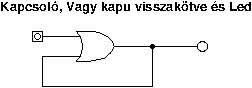
\includegraphics[scale=1.5]{dw/circuit_test5.pdf}
\vspace{-10pt}
\end{center}}
{Tesztelő}
{\vspace{-15pt}
\begin{itemize}
\setlength{\itemsep}{0cm}%
\setlength{\parskip}{0cm}%
\setlength{\itemindent}{-15pt}%
\item Áramkör és komponensek létrehozása
\item szimuláció indítása
\begin{itemize}
\setlength{\itemsep}{0cm}%
\setlength{\parskip}{0cm}%
\setlength{\itemindent}{-35pt}%
\item hálózat kiértékelés indítása
\begin{itemize}
\setlength{\itemsep}{0cm}%
\setlength{\parskip}{0cm}%
\setlength{\itemindent}{-50pt}%
	\item kapcsoló kiértékelése
	\begin{itemize}
	\setlength{\itemsep}{0cm}%
	\setlength{\parskip}{0cm}%
	\setlength{\itemindent}{-65pt}%
		\item kapcsoló állapotának lekérdezése (\textbf{megkérdezi a tesztelőt}, javasolt: 1)
		\item kapcsoló értékének kiadása a vezetékre
	\end{itemize}
	\item kapu kiértékelése
	\begin{itemize}
	\setlength{\itemsep}{0cm}%
	\setlength{\parskip}{0cm}%
	\setlength{\itemindent}{-65pt}%
		\item kapu egyik bemenetének (amelyiken a kapcsoló van) lekérdezése (\textbf{megkérdezi a tesztelőt}, javasolt: 1)
		\item kapu másik bemenetének lekérdezése (\textbf{megkérdezi a tesztelőt}, javasolt: 0)
		\item kapu értékének kiadása a vezetékre (\textbf{megkérdezi a tesztelőt}, javasolt: 1)
	\end{itemize}
	\item node kiértékelése
	\begin{itemize}
	\setlength{\itemsep}{0cm}%
	\setlength{\parskip}{0cm}%
	\setlength{\itemindent}{-65pt}%
		\item node bemenetének lekérdezése (\textbf{megkérdezi a tesztelőt}, javasolt: 1)
		\item node értékének kiadása a vezetékekre (\textbf{megkérdezi a tesztelőt}, javasolt: mindkettőre 1)
	\end{itemize}
	\item led kiértékelése
	\begin{itemize}
	\setlength{\itemsep}{0cm}%
	\setlength{\parskip}{0cm}%
	\setlength{\itemindent}{-65pt}%
		\item led bemenetének lekérdezése (\textbf{megkérdezi a tesztelőt}, javasolt: 1)
	\end{itemize}
\end{itemize}
\item áramkör változásának vizsgálata
\begin{itemize}
\setlength{\itemsep}{0cm}%
\setlength{\parskip}{0cm}%
\setlength{\itemindent}{-50pt}%
	\item kapcsoló változásának vizsgálata (\textbf{megkérdezi a tesztelőt}, javasolt: 1)
	\item kapu változásának vizsgálata (\textit{idáig nem kéne eljutni\ldots})
	\item node változásának vizsgálata (\textit{idáig nem kéne eljutni\ldots})
	\item led változásának vizsgálata (\textit{idáig nem kéne eljutni\ldots})
\end{itemize}
\item áramkör változott, ezért új ciklus
\item hálózat kiértékelés indítása
\begin{itemize}
\setlength{\itemsep}{0cm}%
\setlength{\parskip}{0cm}%
\setlength{\itemindent}{-50pt}%
	\item kapcsoló kiértékelése
	\begin{itemize}
	\setlength{\itemsep}{0cm}%
	\setlength{\parskip}{0cm}%
	\setlength{\itemindent}{-65pt}%
		\item kapcsoló állapotának lekérdezése (\textbf{megkérdezi a tesztelőt}, javasolt: 1)
		\item kapcsoló értékének kiadása a vezetékre
	\end{itemize}
	\item kapu kiértékelése
	\begin{itemize}
	\setlength{\itemsep}{0cm}%
	\setlength{\parskip}{0cm}%
	\setlength{\itemindent}{-65pt}%
		\item kapu egyik bemenetének (amelyiken a kapcsoló van) lekérdezése (\textbf{megkérdezi a tesztelőt}, javasolt: 1)
		\item kapu másik bemenetének lekérdezése (\textbf{megkérdezi a tesztelőt}, javasolt: 1)
		\item kapu értékének kiadása a vezetékre (\textbf{megkérdezi a tesztelőt}, javasolt: 1)
	\end{itemize}
\item node kiértékelése
	\begin{itemize}
	\setlength{\itemsep}{0cm}%
	\setlength{\parskip}{0cm}%
	\setlength{\itemindent}{-65pt}%
		\item node bemenetének lekérdezése (\textbf{megkérdezi a tesztelőt}, javasolt: 1)
		\item node értékének kiadása a vezetékekre (\textbf{megkérdezi a tesztelőt}, javasolt: mindkettőre 1)
	\end{itemize}	
	\item led kiértékelése
	\begin{itemize}
	\setlength{\itemsep}{0cm}%
	\setlength{\parskip}{0cm}%
	\setlength{\itemindent}{-65pt}%
		\item led bemenetének lekérdezése (\textbf{megkérdezi a tesztelőt}, javasolt: 1)
	\end{itemize}
\end{itemize}
\item áramkör változásának vizsgálata
\begin{itemize}
\setlength{\itemsep}{0cm}%
\setlength{\parskip}{0cm}%
\setlength{\itemindent}{-50pt}%
	\item kapcsoló változásának vizsgálata (\textbf{megkérdezi a tesztelőt}, javasolt: 0)
	\item kapu változásának vizsgálata (\textbf{megkérdezi a tesztelőt}, javasolt: 0)
	\item node változásának vizsgálata (\textbf{megkérdezi a tesztelőt}, javasolt: 0)
	\item led változásának vizsgálata (\textbf{megkérdezi a tesztelőt}, javasolt: 0)
\end{itemize}
\item áramkör nem változott, stabil állapot
\item FF-okat véglegesítjük (nem történik semmi, mert nincs FF)
\item jelgenerátorokat léptetjük (nem történik semmi, mert nincs jelgenerátor)
\item stacionárius állapot, szimuláció vége
\end{itemize}
\end{itemize}
\vspace{-15pt}}

\section{Architektúra}

\section{A szkeleton kezelői felületének terve, dialógusok}
Az általunk elkészített szkeleton egy program váz melynek felülete egy egyszerű konzolos megjelenítési felület, amely alkalmas arra, hogy a use case-k által leírt teszteseteket bemutassuk. Az egyes tesztesetek a neki megfelelő use case sorszámával van elnevezve, így program indítás után egy szám bevitelét követően a kiválasztott teszteset lefut. 
A teszteset futása közben kiír minden objektumot amin metódust hív, illetve kiírja a metódus nevét a paraméterekkel együtt, majd a visszatérési értéket. Ez azért lehetséges, mert a szkeleton már tartalmazza az elkészítendő szoftver összes fontos osztályát és metódusát, azonban az üzleti logikát még nem. Így könnyen eldönthető, hogy a use case-nek megfelelően viselkedik a program és továbbiakban képes lesz-e megfelelően működni.
A tesztelési folyamat során döntési helyzet léphet fel. Ilyenkor a program felteszi a kérdést, majd a kapott válasz alapján folytatja a további futást. Ezzel csökkentjük a tesztesetek számát, anélkül, hogy bizonyos esetek kimaradnának a tesztelés alól. 
Futás közben megjegyzés formájában a program tájékoztat bizonyos fontosabb lépésekről (például inicializálás), vagy a megértést segítő egyéb dolgokról.
Az elvárás, hogy a szkeleton a szekvenciadiagramok által leírt működést mutassa. A program egyszerű és könnyen összehasonlítható formában írja ki a működését, amelyet könnyen összevethetjük a szekvencia diagrammokkal.

\subsection{Program üzeneteinek formátuma}

A program a következő eseményeket jelzi ki:
\begin{itemize}
\item Konstruktor hívás.\\
	  Formátum: \texttt{CREATE osztálynév objektumnév}\\
	  Példa: \texttt{CREATE Circuit circuit}
\item Tagfüggvény hívás.\\
	  Formátum: \texttt{CALL objektumnév.metódus(paraméterek)}\\
	  Példa: \texttt{CALL wire.setValue(Value.TRUE)}
\item Konstruktor/tagfüggvény visszatér\\
	  Formátum: \texttt{RETURN} vagy \texttt{RETURN objektumnév/érték}\\
	  Ha van visszatérési érték az kétféle lehet: referencia valamelyik objektumra (ekkor az objektumnevet írjuk ki), vagy egy konkrét érték (ilyenkor az értéket, pl: \texttt{false}).
\item Kérdés a felhasználónak.\\
	  Formátum: \texttt{QUESTION objektumnév üzenet? [opciók]}\\
	  Példa: \texttt{QUESTION wire vezetéken lévő érték? [0/1]}\\
	  Objektumnév annak az objektumnak a neve, aki kérdezi a felhasználót. Az opciókban lévő elemek \texttt{/} jellel vannak elválasztva. Addig nem megy tovább a program, amíg nem ezek közül kap választ.
\item Megjegyzés kijelzése.\\
	Formátum: \texttt{\# üzenet}
\end{itemize}

Formátum bemutatásához egy összetettebb példa:

\begin{verbatim}
CALL simulation.start()
  CALL circuit.doEvaluationCycle()
    CALL toggle.evaluate()
      QUESTION toggle állapot? [0/1] 1
      CALL wire.setValue(Value.TRUE)
      RETURN
    RETURN
    CALL led.evaluate()
      CALL wire.getValue()
        QUESTION wire vezetéken lévő érték? [0/1] 1
      RETURN Value.TRUE
    RETURN
  RETURN
  CALL circuit.isChanged()
    CALL toggle.isChanged()
      QUESTION toggle változott? [0/1] 1
    RETURN true
  RETURN true
  CALL circuit.doEvaluationCycle()
    CALL toggle.evaluate()
      QUESTION toggle állapot? [0/1] 1
      CALL wire.setValue(Value.TRUE)
      RETURN
    RETURN
    CALL led.evaluate()
      CALL wire.getValue()
        QUESTION wire vezetéken lévő érték? [0/1] 1
      RETURN Value.TRUE
    RETURN
  RETURN
  CALL circuit.isChanged()
    CALL toggle.isChanged()
      QUESTION toggle változott? [0/1] 0
    RETURN false
    CALL led.isChanged()
      QUESTION led változott? [0/1] 0
    RETURN false
  RETURN false
  CALL circuit.commitFlipFlops()
  RETURN
  CALL circuit.stepGenerators()
  RETURN
RETURN true
\end{verbatim}

\section{Szekvencia diagramok a belső működésre}

\begin{figure}[H]
\begin{center}
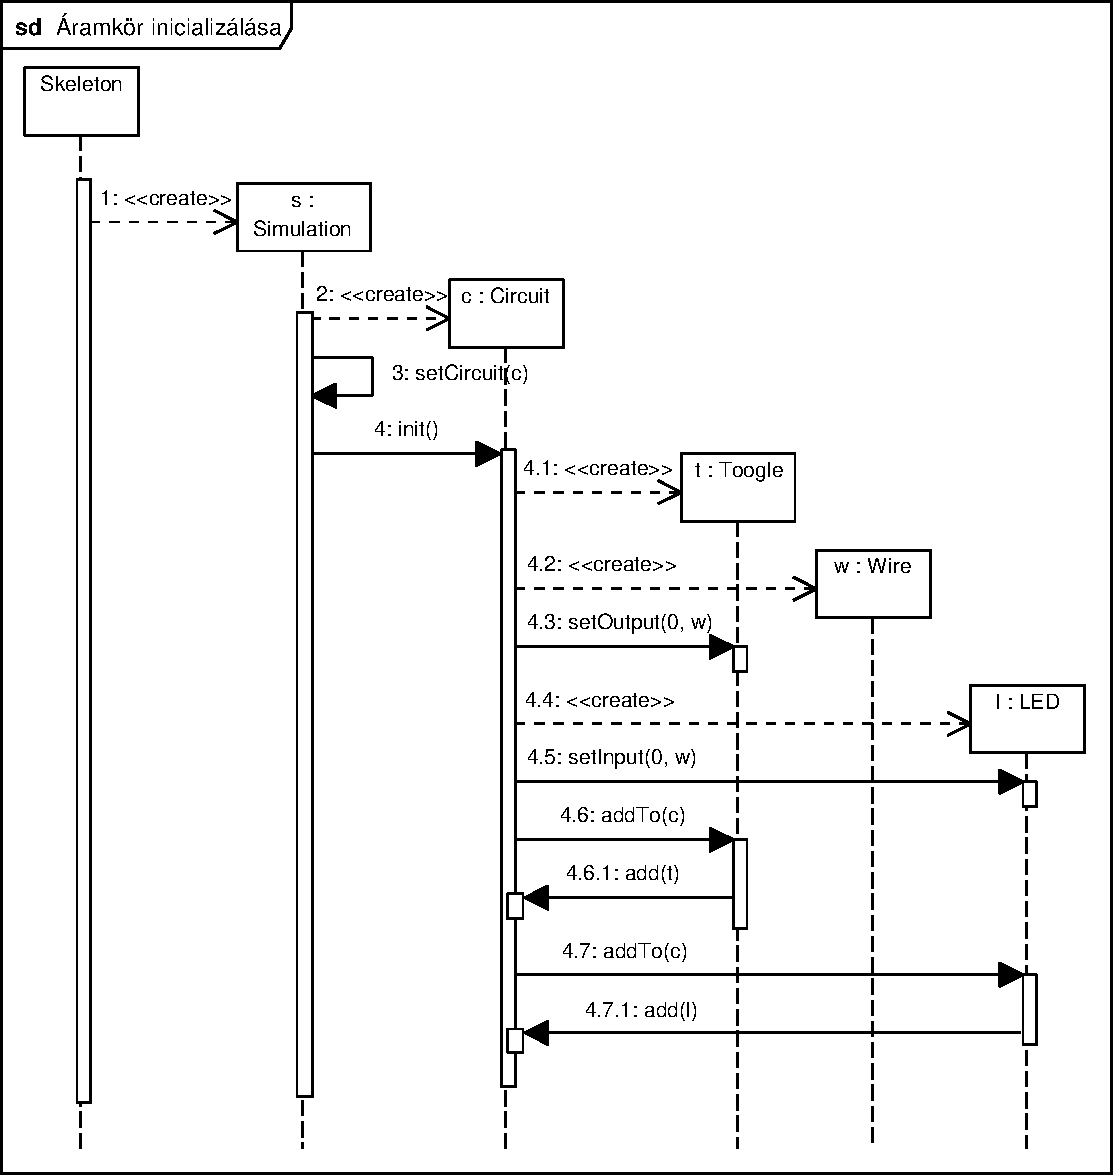
\includegraphics[width=17cm]{chapters/chapter05/imgs/init.pdf}
\caption{Áramkör inicializálása}
\label{fig:init}
\end{center}
\end{figure}

\begin{figure}[H]
\begin{center}
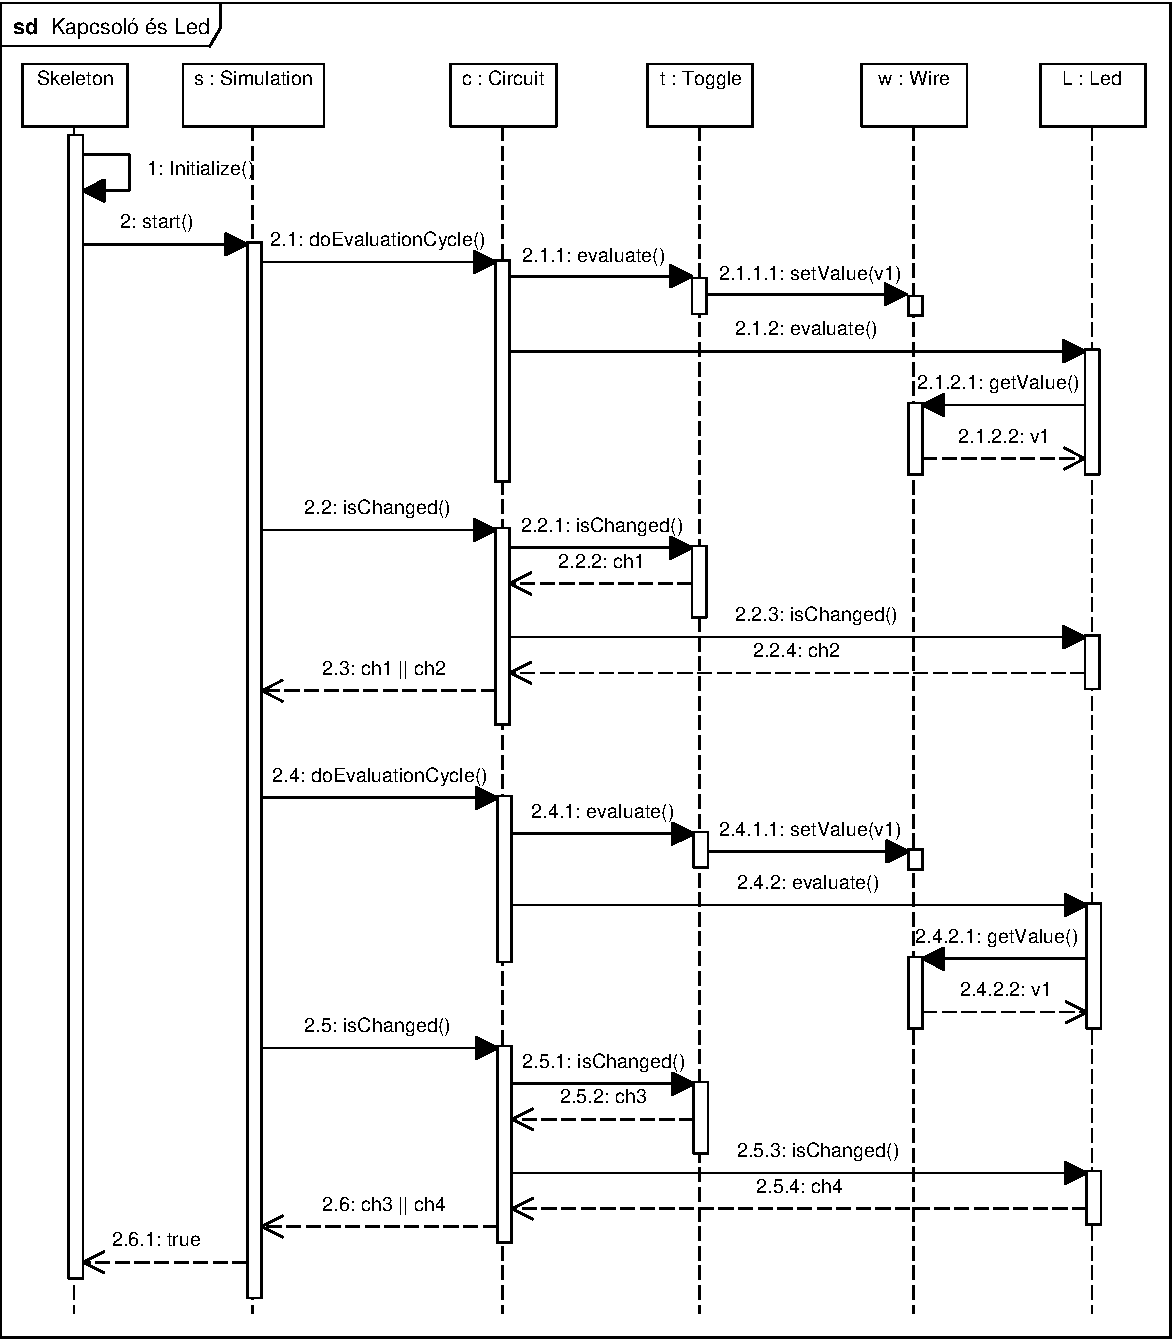
\includegraphics[width=17cm]{chapters/chapter05/imgs/test1.pdf}
\caption{Kapcsoló és Led}
\label{fig:test1}
\end{center}
\end{figure}

\begin{figure}[H]
\begin{center}
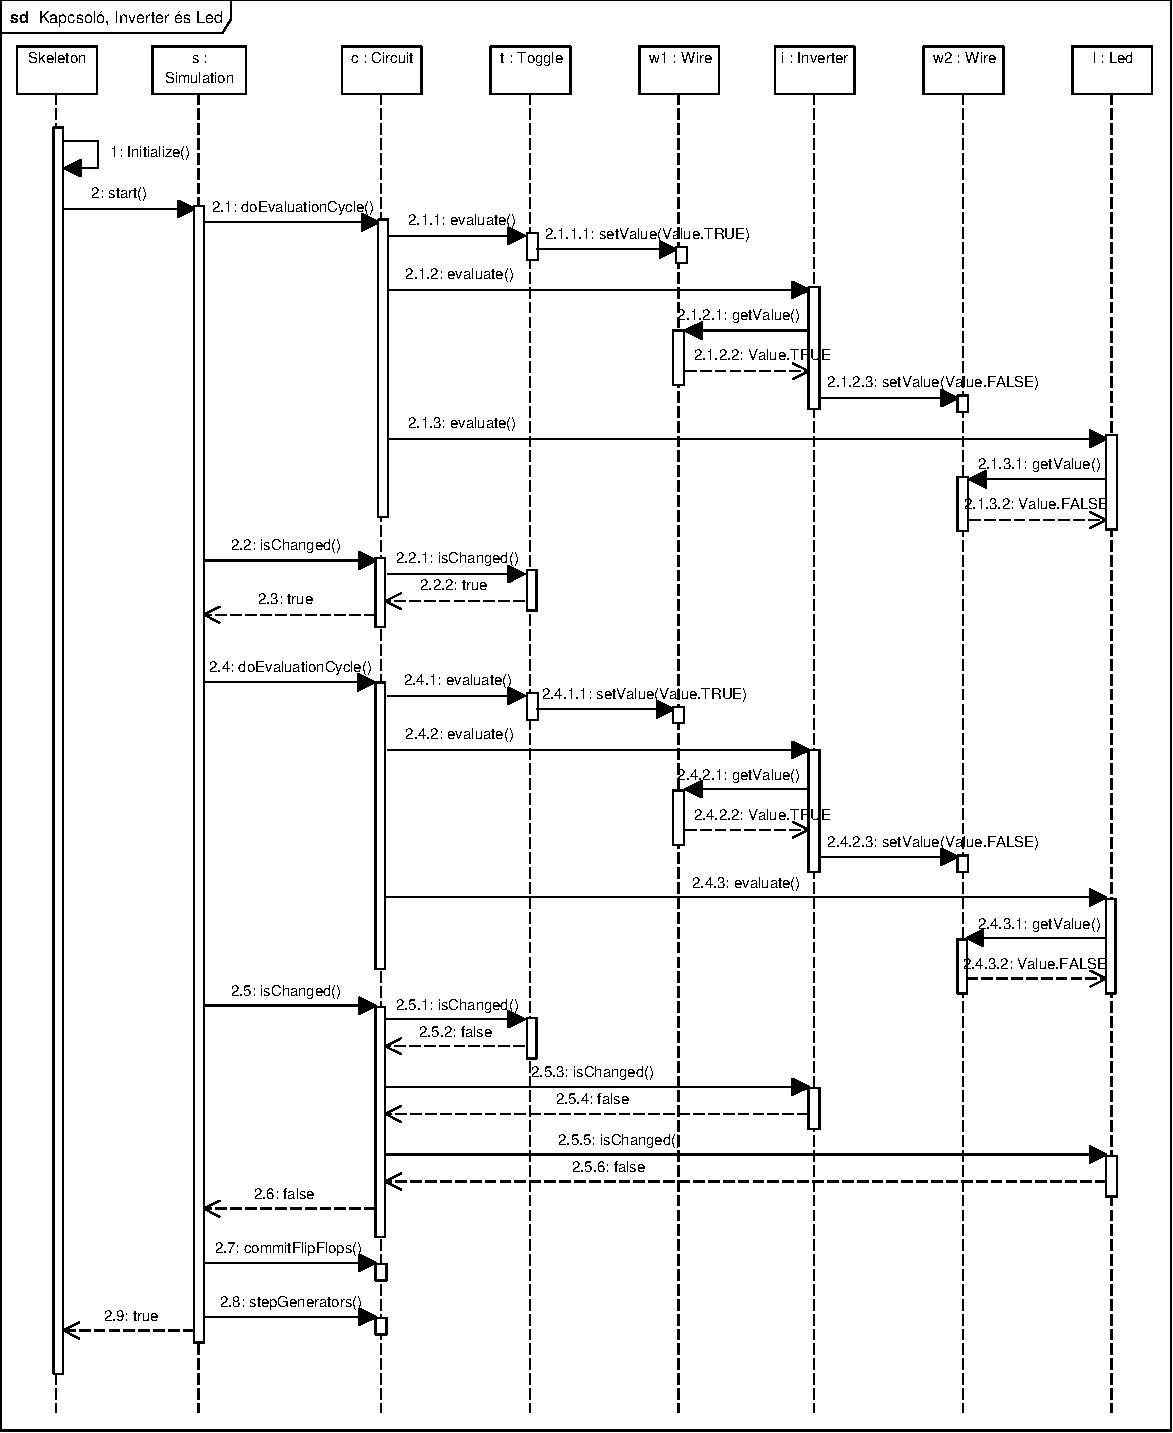
\includegraphics[width=17cm]{chapters/chapter05/imgs/test2.pdf}
\caption{Kapcsoló, Inverter és Led}
\label{fig:test2}
\end{center}
\end{figure}

\begin{figure}[H]
\begin{center}
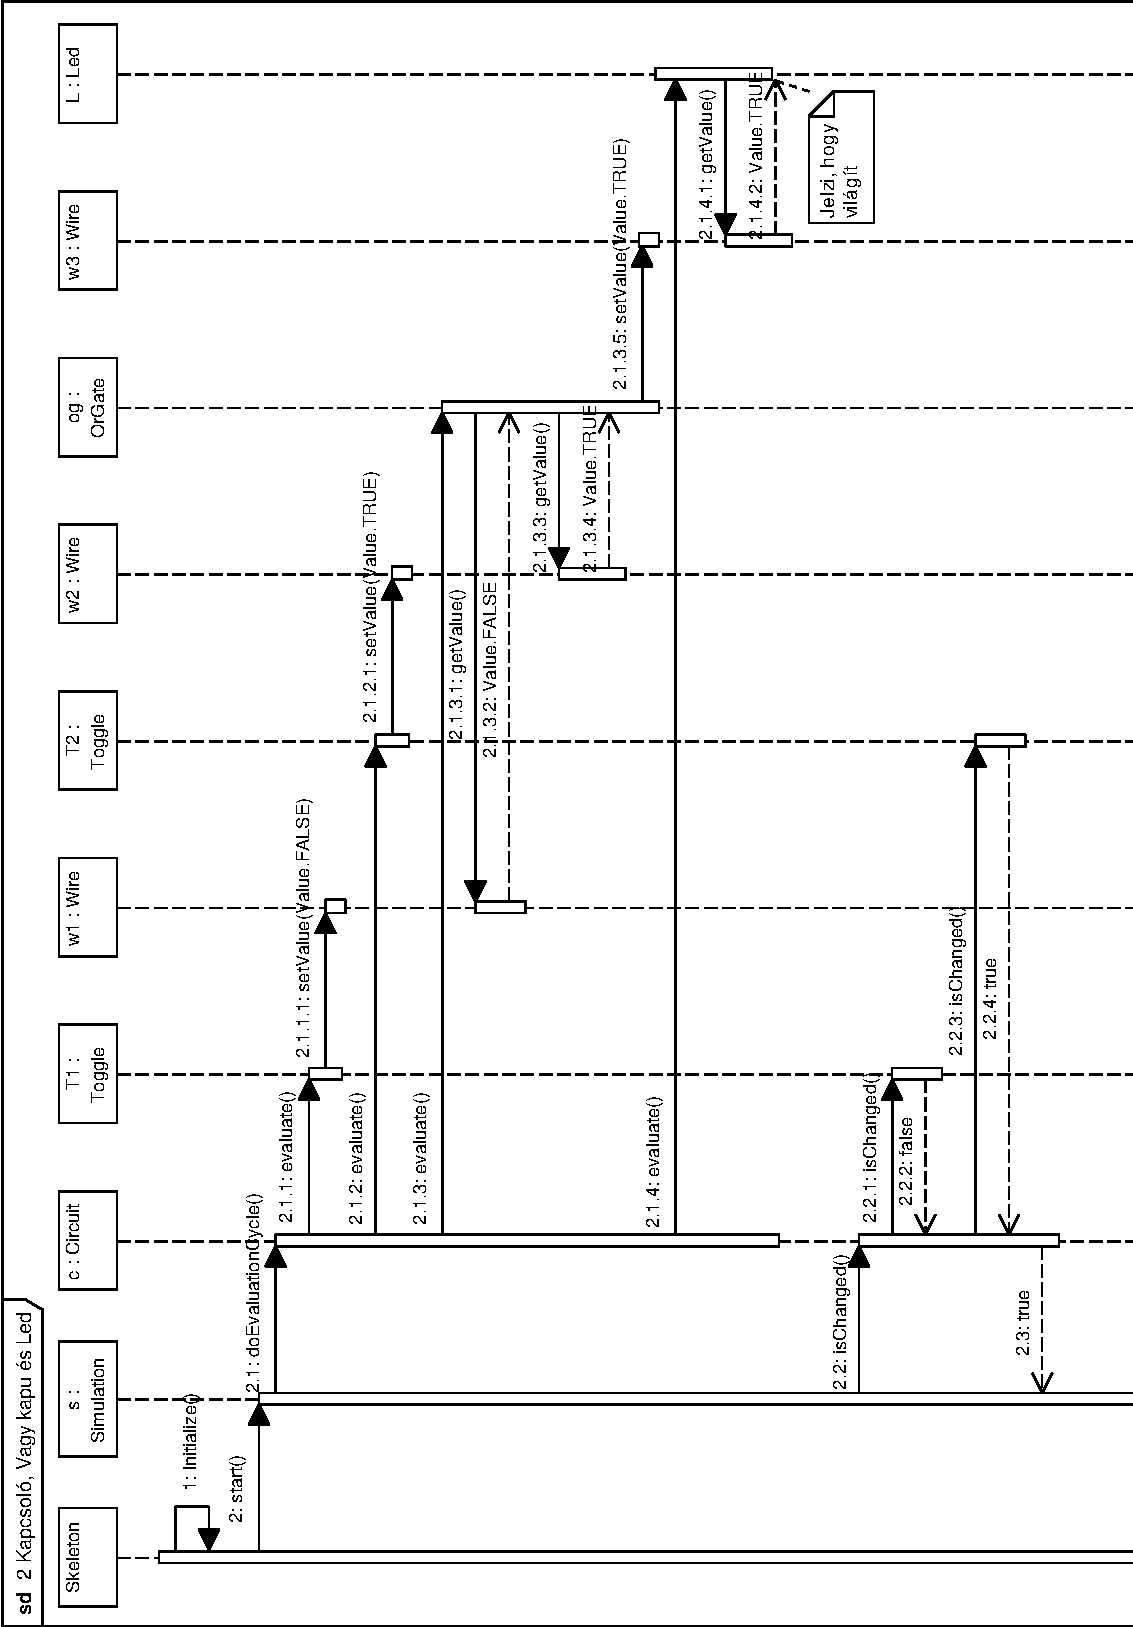
\includegraphics[width=16cm]{chapters/chapter05/imgs/test3-1.pdf}
\caption{2 Kapcsoló, Vagy kapu és Led (1. rész)}
\label{fig:test3_1}
\end{center}
\end{figure}

\begin{figure}[H]
\begin{center}
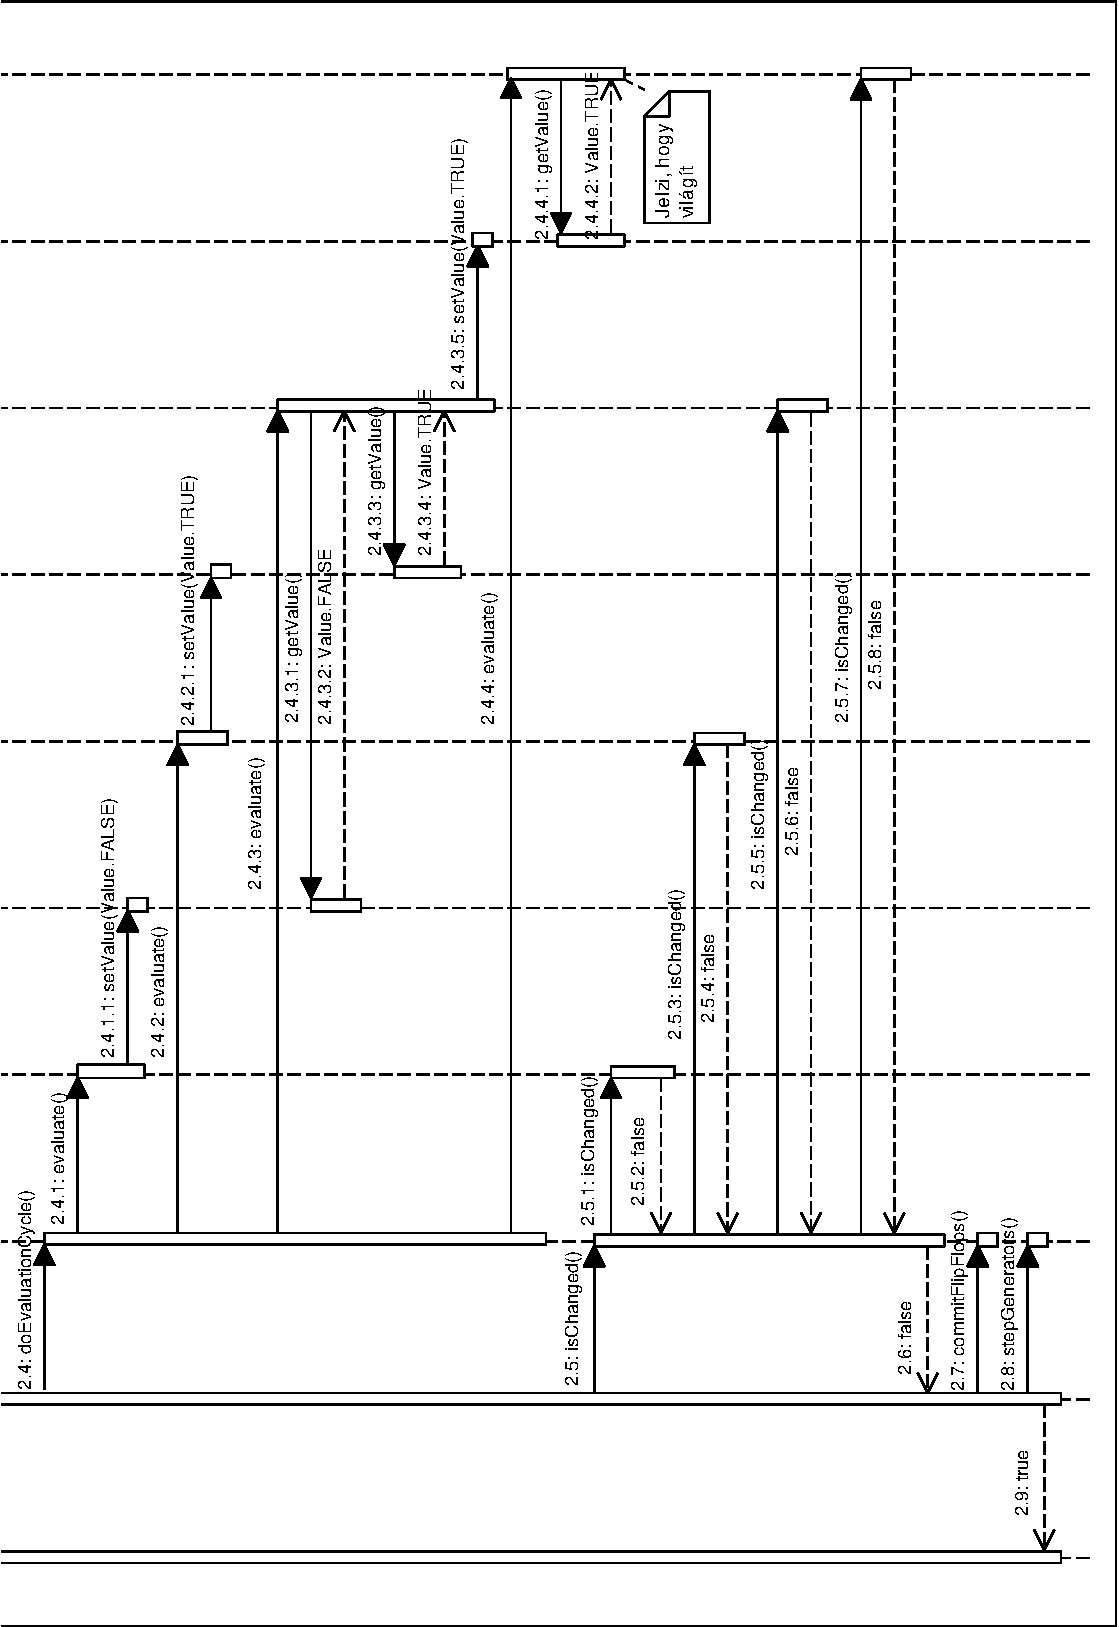
\includegraphics[width=16cm]{chapters/chapter05/imgs/test3-2.pdf}
\caption{2 Kapcsoló, Vagy kapu és Led (2. rész)}
\label{fig:test3_2}
\end{center}
\end{figure}

\begin{figure}[H]
\begin{center}
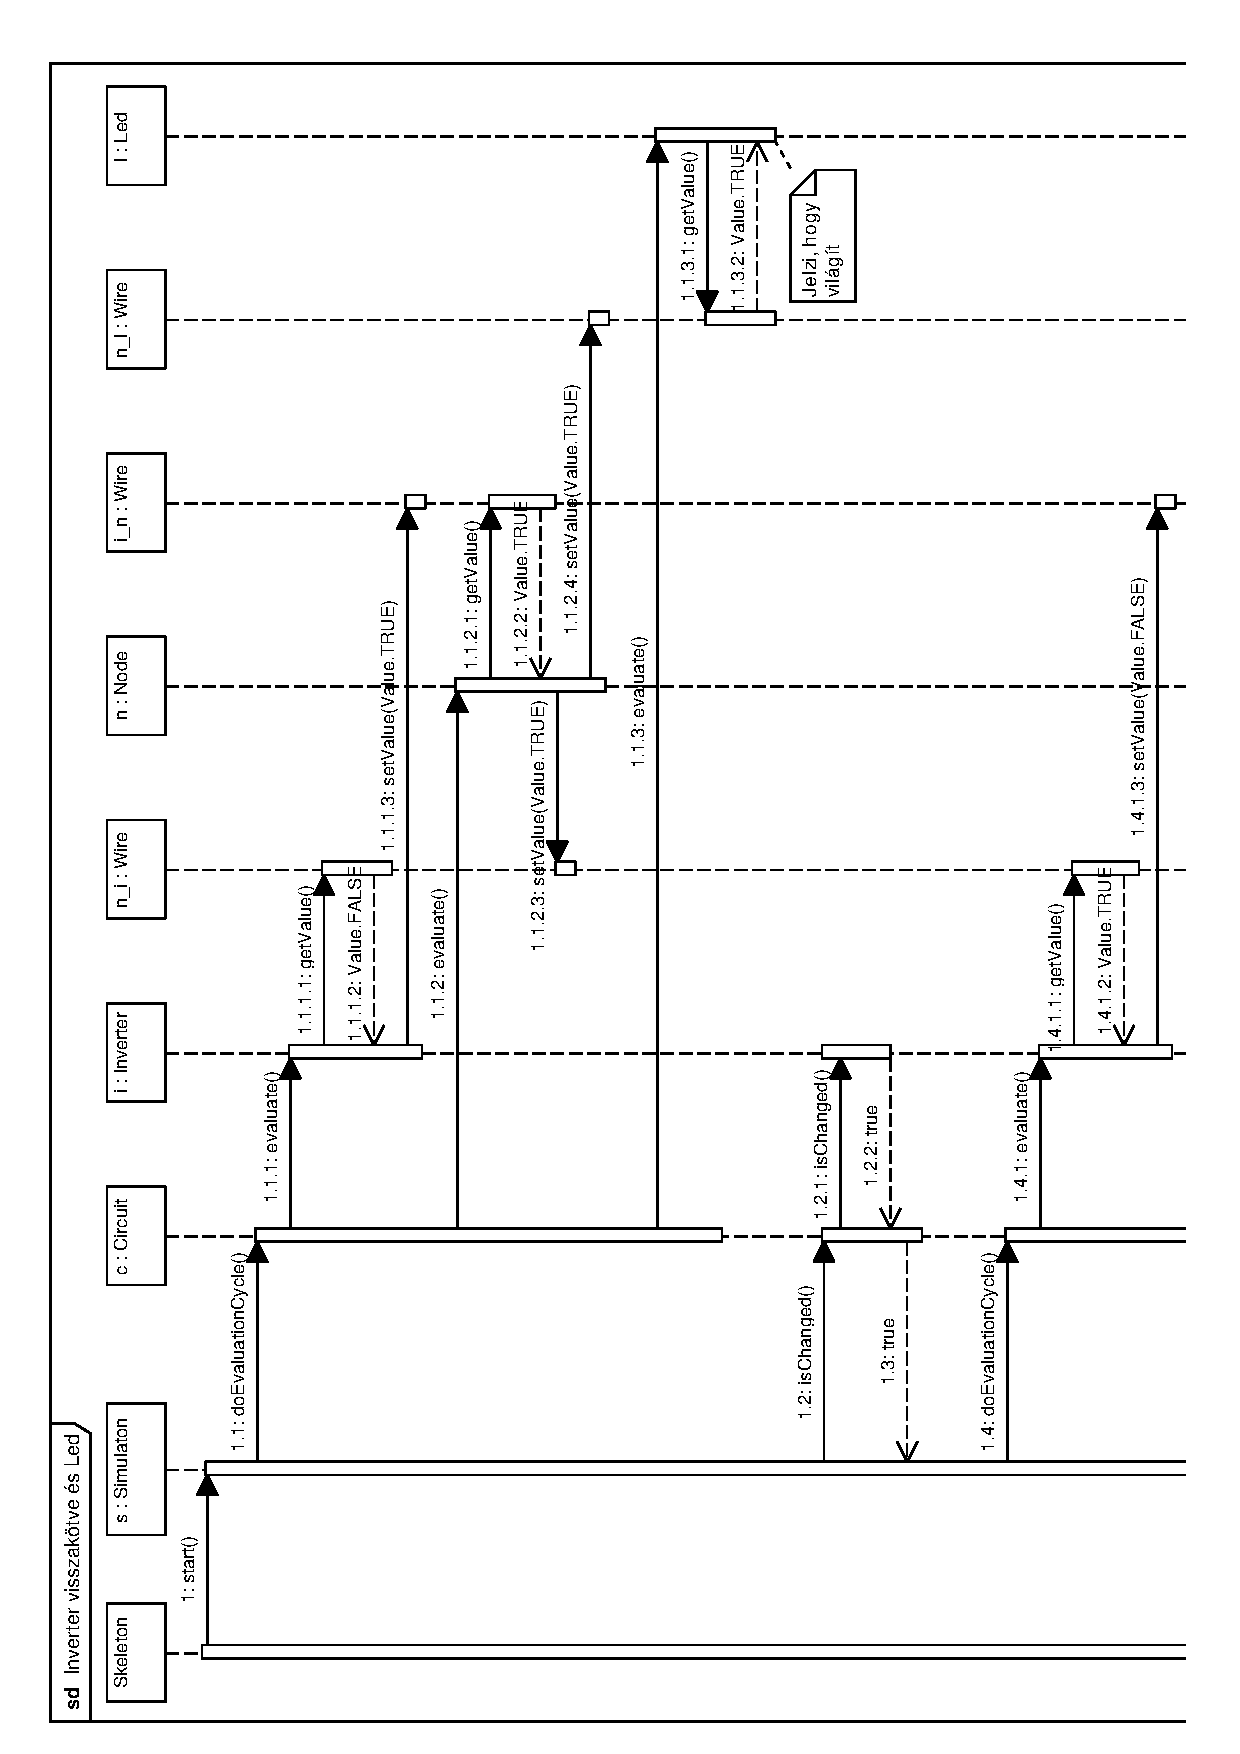
\includegraphics[height=23cm]{chapters/chapter05/imgs/test4-1.pdf}
\caption{Inverter visszakötve és Led (1. rész)}
\label{fig:test4_1}
\end{center}
\end{figure}

\begin{figure}[H]
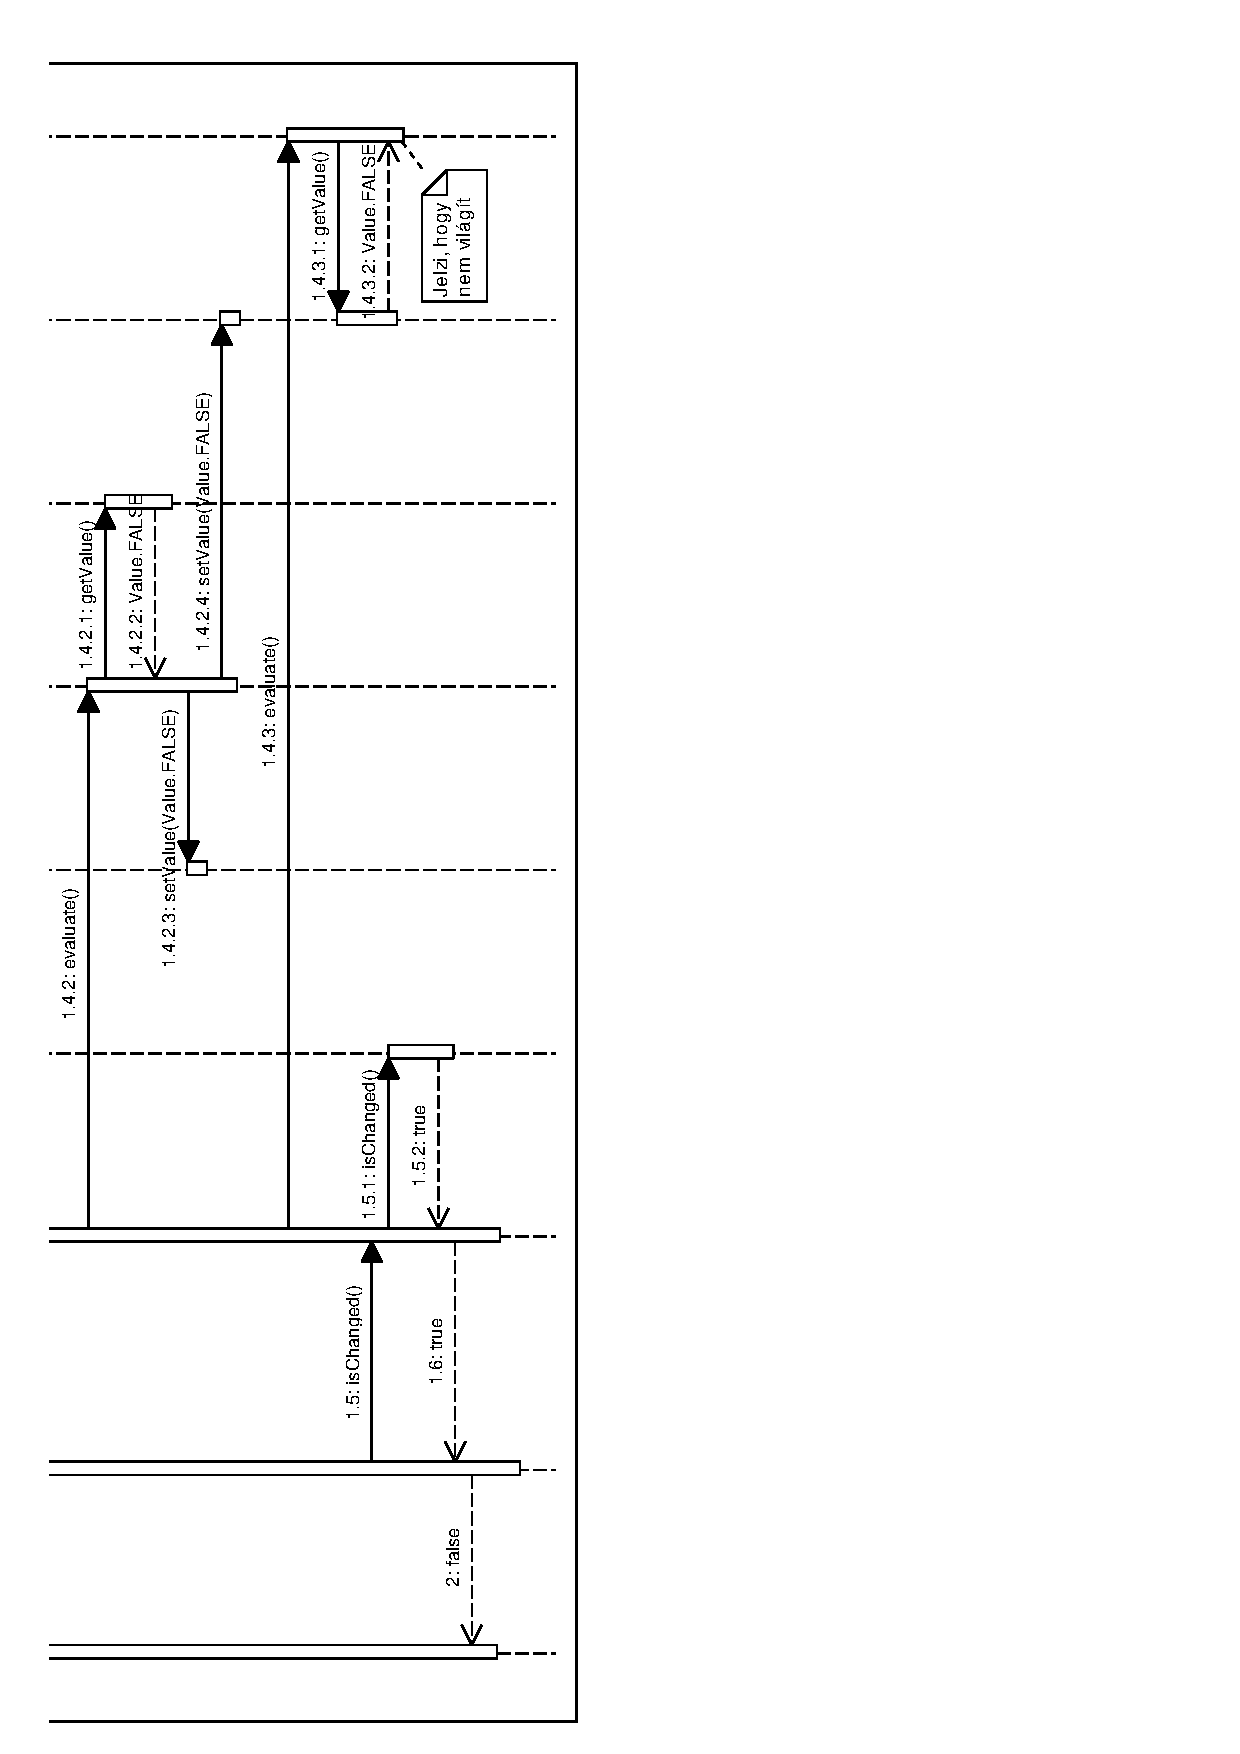
\includegraphics[height=23cm]{chapters/chapter05/imgs/test4-2.pdf}
\caption{Inverter visszakötve és Led (2. rész)}
\label{fig:test4_2}
\end{figure}


\begin{figure}[H]
\begin{center}
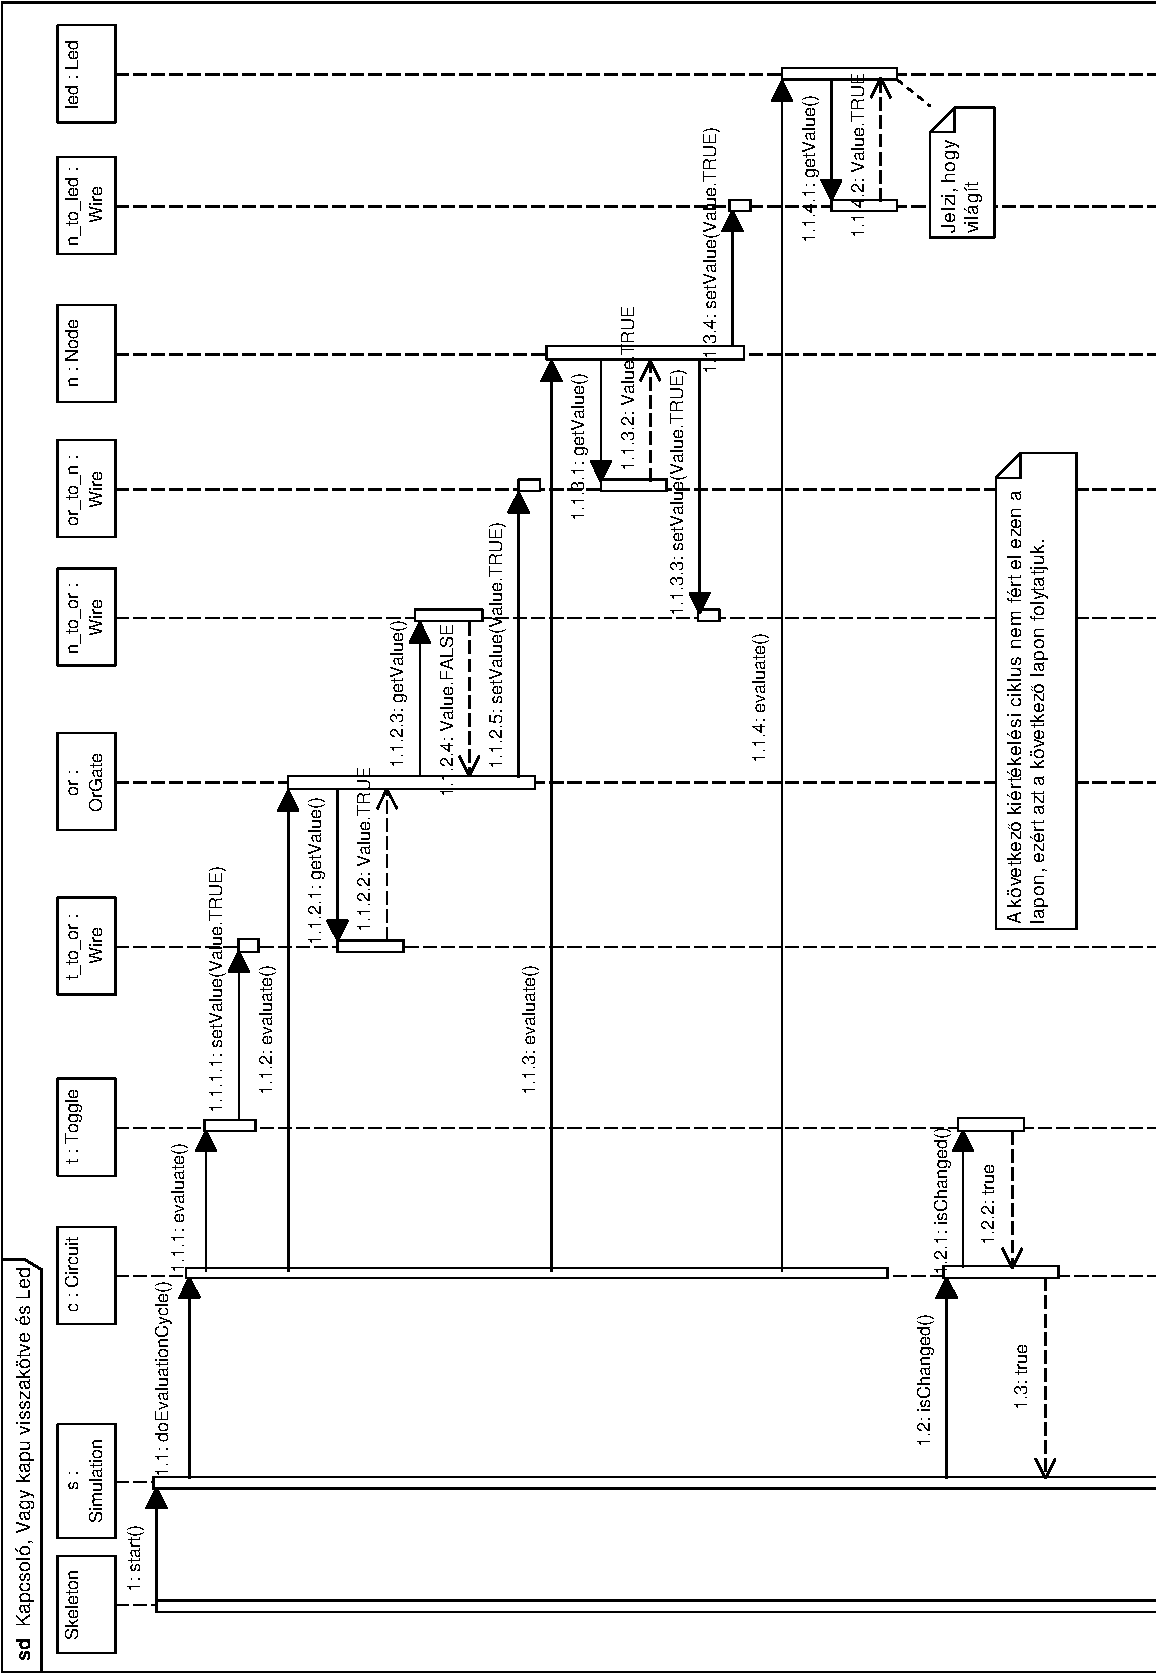
\includegraphics[width=16cm]{chapters/chapter05/imgs/test5-1.pdf}
\caption{Kapcsoló, Vagy kapu visszakötve és Led (1. rész)}
\label{fig:test5_1}
\end{center}
\end{figure}

\begin{figure}[H]
\begin{center}
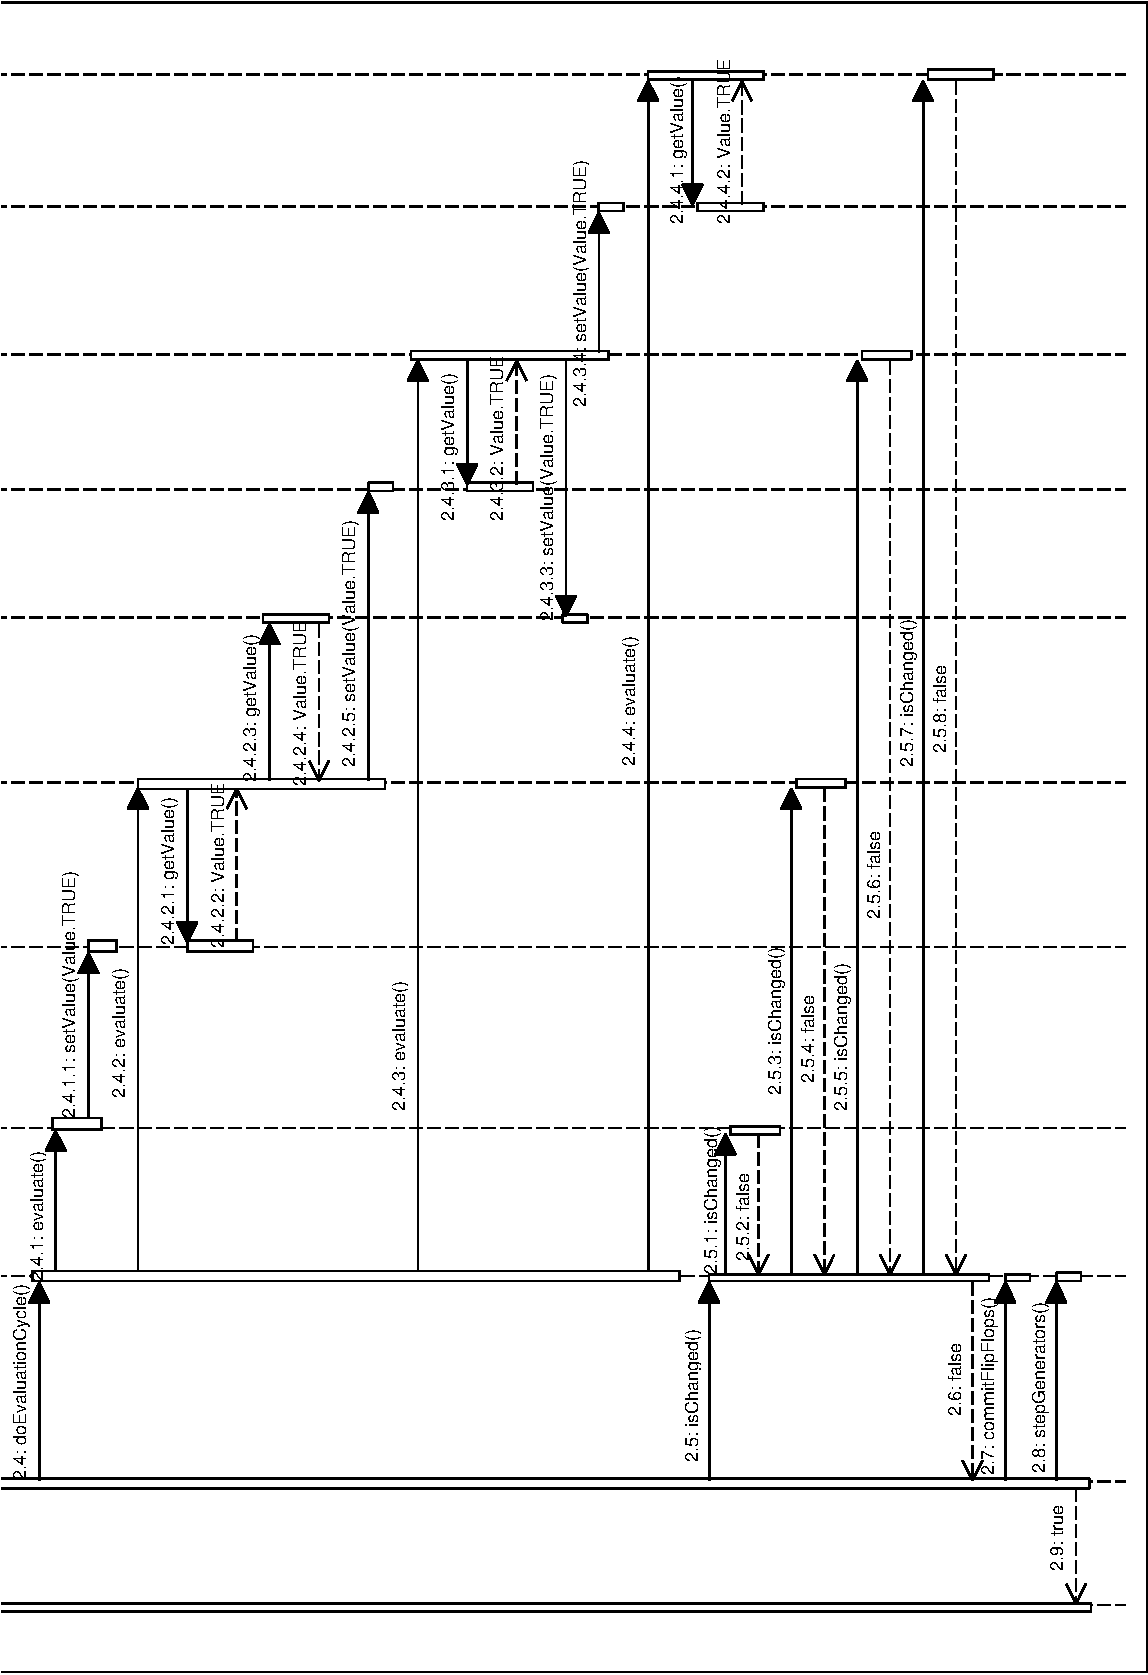
\includegraphics[width=16cm]{chapters/chapter05/imgs/test5-2.pdf}
\caption{Kapcsoló, Vagy kapu visszakötve és Led (2. rész)}
\label{fig:test5_2}
\end{center}
\end{figure}
%% Szglab4
% ===========================================================================
%
\section{Napló}

\begin{naplo}

\bejegyzes
{2010.03.11.~14:00~}
{1,5 óra}
{Kriván B.}
{Javasolt módosítások elvégzése az előző fejezetben, rövid errate készítése jelen fejezet elé.}

\bejegyzes
{2010.03.12.~00:00~}
{2 óra}
{Péter T.}
{Use-casek leírása szöveges formátumban}

\bejegyzes
{2010.03.12.~09:30~}
{30 perc}
{Kriván B.}
{Use-case diagram megrajzolása}

\bejegyzes
{2010.03.12.~10:00~}
{2 óra}
{Kriván B.}
{Use-casek leírásának \LaTeX{} formátumra való alakítása, apróbb finomítások}

\bejegyzes
{2010.03.13.~16:00~}
{2 óra}
{Apagyi G.}
{Első 3 (\ref{fig:init}, \ref{fig:test1}, \ref{fig:test2}) szekvenciadiagram megrajzolása}

\bejegyzes
{2010.03.13.~17:00~}
{1 óra}
{Kriván B.\newline
Dévényi A.\newline
Péter T.}
{Értekezlet\newline
Döntés: kimeneti és bemeneti értékeket egyaránt bekérjük a felhasználótól, ciklusok száma: 2 (elégnek kell lennie ezeknél az áramköröknél), nagy diagramokat félbevágjuk}

\bejegyzes
{2010.03.13.~18:00~}
{2 óra}
{Kriván B.}
{\ref{fig:init}, \ref{fig:test1}, és \ref{fig:test2} diagramok és az utolsó (\ref{fig:test5_1} és \ref{fig:test5_2}) szekvenciadiagram formázása, tömörítése, leírások frissítése}

\bejegyzes
{2010.03.13.~18:00~}
{3 óra}
{Dévényi A.}
{\ref{fig:test3_1} és \ref{fig:test3_2} diagram formázása, tömörítése és \aref{fig:test4_1} és \ref{fig:test4_2} szekvenciadiagram megrajzolása leírások frissítése}

\bejegyzes
{2010.03.13.~18:00~}
{1 óra}
{Jákli G.}
{5.4-es fejezet megírása}

\end{naplo}



%\setcounter{chapter}{5} 
%% Szglab4
% ===========================================================================
%
\chapter{Szkeleton beadás}

\thispagestyle{fancy}

\section{Fordítási és futtatási útmutató}
\comment{A feltöltött program fordításával és futtatásával kapcsolatos útmutatás. Ennek tartalmaznia kell leltárszerűen az egyes fájlok pontos nevét, méretét byte-ban, keletkezési idejét, valamint azt, hogy a fájlban mi került megvalósításra.}

\subsection{Fájllista}

\begin{fajllista}

\fajl
{compile.bat} % Kezdet
{250 byte} % Idptartam
{2009.10.10~18:05~} % Résztvevők
{Fordításra használt batch fájl} % Leírás
\fajl
{doc.bat} % Kezdet
{250 byte} % Idptartam
{2009.10.10~18:05~} % Résztvevők
{Dokumentum generálására készített batch fájl} % Leírás
\fajl
{run.bat} % Kezdet
{250 byte} % Idptartam
{2009.10.10~18:05~} % Résztvevők
{Indításhoz használt batch fájl} % Leírás

\fajl
{src/logsim/Skeleton.java} % Kezdet
{250 byte} % Idptartam
{2009.10.10~18:05~} % Résztvevők
{Menüt tartalmazza. A felhasználó választása alapján a megfelelő tesztesetet elindítja} % Leírás

\fajl
{src/logsim/log/Loggable.java} % Kezdet
{250 byte} % Idptartam
{2009.10.10~18:05~} % Résztvevők
{Loggolást segítő interfész} % Leírás

\fajl
{src/logsim/log/\newline
LoggableInt.java} % Kezdet
{250 byte} % Idptartam
{2009.10.10~18:05~} % Résztvevők
{Wrapper osztály az int típus köré, mely lehetővé teszi az intek loggolását} % Leírás

\fajl
{src/logsim/log/Logger.java} % Kezdet
{250 byte} % Idptartam
{2009.10.10~18:05~} % Résztvevők
{Loggolást megvalósító osztály} % Leírás

\fajl
{src/logsim/model/Circuit.java} % Kezdet
{250 byte} % Idptartam
{2009.10.10~18:05~} % Résztvevők
{Az áramkört megvalósító osztály} % Leírás

\fajl
{src/logsim/model/\newline
Simulation.java} % Kezdet
{250 byte} % Idptartam
{2009.10.10~18:05~} % Résztvevők
{A szimulációt megvalósító osztály} % Leírás

\fajl
{src/logsim/model/Value.java} % Kezdet
{250 byte} % Idptartam
{2009.10.10~18:05~} % Résztvevők
{Az áramkörben előforduló értkékeket tartalmazó osztály} % Leírás

\fajl
{src/logsim/model/component/\newline
AbstractComponent.java} % Kezdet
{250 byte} % Idptartam
{2009.10.10~18:05~} % Résztvevők
{Az alkatrészek absztrakt ősosztálya} % Leírás

\fajl
{src/logsim/model/component/\newline
DisplayComponent.java} % Kezdet
{250 byte} % Idptartam
{2009.10.10~18:05~} % Résztvevők
{Megjelenítő típusú alkatrészek absztrakt ősosztálya} % Leírás

\fajl
{src/logsim/model/component/\newline
SourceComponent.java} % Kezdet
{250 byte} % Idptartam
{2009.10.10~18:05~} % Résztvevők
{Forrás típusú alkatrészek absztrakt ősosztálya} % Leírás

\fajl
{src/logsim/model/component/\newline
Wire.java} % Kezdet
{250 byte} % Idptartam
{2009.10.10~18:05~} % Résztvevők
{Vezetéket megvalósító osztály} % Leírás

\fajl
{src/logsim/model/component/\newline
impl/Inverter.java} % Kezdet
{250 byte} % Idptartam
{2009.10.10~18:05~} % Résztvevők
{Az inverter alkatrészt megvalósító osztály} % Leírás

\fajl
{src/logsim/model/component/\newline
impl/Led.java} % Kezdet
{250 byte} % Idptartam
{2009.10.10~18:05~} % Résztvevők
{A led megjelenítőt megvalósító osztály} % Leírás

\fajl
{src/logsim/model/component/\newline
impl/Node.java} % Kezdet
{250 byte} % Idptartam
{2009.10.10~18:05~} % Résztvevők
{Csomópont alkatrészt megvalósító osztály} % Leírás

\fajl
{src/logsim/model/component/\newline
impl/OrGate.java} % Kezdet
{250 byte} % Idptartam
{2009.10.10~18:05~} % Résztvevők
{VAGY kaput megvalósító osztály} % Leírás

\fajl
{src/logsim/model/component/\newline
impl/Toggle.java} % Kezdet
{250 byte} % Idptartam
{2009.10.10~18:05~} % Résztvevők
{A kapcsoló forrást megvalósító osztály} % Leírás

\fajl
{src/logsim/model/skeleton/\newline
Circuit1.java} % Kezdet
{250 byte} % Idptartam
{2009.10.10~18:05~} % Résztvevők
{Az első tesztesetet tartalmazó osztály} % Leírás

\fajl
{src/logsim/model/skeleton/\newline
Circuit2.java} % Kezdet
{250 byte} % Idptartam
{2009.10.10~18:05~} % Résztvevők
{A második tesztesetet tartalmazó osztály} % Leírás

\fajl
{src/logsim/model/skeleton/\newline
Circuit3.java} % Kezdet
{250 byte} % Idptartam
{2009.10.10~18:05~} % Résztvevők
{A harmadik tesztesetet tartalmazó osztály} % Leírás

\fajl
{src/logsim/model/skeleton/\newline
Circuit4.java} % Kezdet
{250 byte} % Idptartam
{2009.10.10~18:05~} % Résztvevők
{A negyedik tesztesetet tartalmazó osztály} % Leírás

\fajl
{src/logsim/model/skeleton/\newline
Circuit5.java} % Kezdet
{250 byte} % Idptartam
{2009.10.10~18:05~} % Résztvevők
{Az ötödik tesztesetet tartalmazó osztály} % Leírás

\end{fajllista}

\subsection{Fordítás}
A hibamentes és minél inkább gördülékenyebb fordítás érdekében létrehoztunk egy compile.bat nevezetű batch fájlt, mely a projekt főkönyvtárában található. Projekt főkönytára az, amelyik batch fájlokat tartalmaz és a "src" nevezetű mappát, melyben a program forráskódja található. Szükség estén kézzel kell módosítani a batch file " set C="C:\Program Files\Java\jdk1.6.0_21\bin\" " sorát, attól függően, hogy a gépen éppen melyik Java JDK verzió található!

A compile.bat fájl az alábbi parancsokat hajtja végre:
\lstset{escapeinside=`', xleftmargin=10pt, frame=single, basicstyle=\ttfamily\footnotesize, language=sh}
\begin{lstlisting}
@echo off
set C="C:\Program Files\Java\jdk1.6.0_21\bin\"
cd src
%C%\javac logsim\Skeleton.java
cd..
if not errorlevel 1 echo Forditas sikeres
pause
\end{lstlisting}
Ha hibamentes volt a fordítás, azt a "Fordítás sikeres" kimenettel értesíti a felhasználót.



A fordítás sikeressége után, lehetőség van a dokumentáció legenerálására is. Ehhez felhasználható a főkönyvtárban található doc.bat batch fájl.
Szükség estén kézzel kell módosítani a batch file " set C="C:\Program Files\Java\jdk1.6.0_21\bin\" " sorát, attól függően, hogy a gépen éppen melyik Java JDK verzió található!
A batch fájl az alábbi parancsokat hajtja végre:
\lstset{escapeinside=`', xleftmargin=10pt, frame=single, basicstyle=\ttfamily\footnotesize, language=sh}
\begin{lstlisting}
@echo off
set C="C:\Program Files\Java\jdk1.6.0_21\bin\"
cd src
%C%\javadoc logsim logsim.log logsim.model logsim.model.component logsim.model.component.impl 
 logsim.model.component.impl logsim.model.skeleton -d ..\documents
cd..
if not errorlevel 1 echo Dokumentum generalas sikeres volt. 
pause
\end{lstlisting}
Ha a dokumentum generálás sikeres volt, akkor a documents nevezetű mappában megtaláhatóak a kívánt dokumentumok.




\subsection{Futtatás}
A futtatás megkönnyításe érdekében elkészítettük a run.bat batch fájlt.
Szükség estén kézzel kell módosítani a batch file " set C="C:\Program Files\Java\jdk1.6.0_21\bin\" " sorát, attól függően, hogy a gépen éppen melyik Java JDK verzió található!
Ez az alábbi parancsokat hajtja végre:
\lstset{escapeinside=`', xleftmargin=10pt, frame=single, basicstyle=\ttfamily\footnotesize, language=sh}
\begin{lstlisting}
@echo off
set C="C:\Program Files\Java\jdk1.6.0_21\bin\"
cd src
%C%\java logsim.Skeleton
\end{lstlisting}
Az "src" könyvtárból elindítja az előzőleg lefordított programot.


\section{Értékelés}
\comment{A projekt kezdete óta az értékelésig eltelt időben tagokra bontva, százalékban.}

Csapatunk már a múlt félévben kialakult, így nem voltunk ismeretlenek egymás számára, ismertük egymás képességeit. Az elején hamar egyeszségre jutottunk, hogy miként fog történni a kommunikáció a csapaton belül és milyen módon tároljuk az elkészült anyagokat, úgy, hogy mindig mindenki a legfrissebb fájlokhoz férhessen hozzá. 
A közös munka elején mégis gondot okozott számunkra a csapatban dolgozás. Ezt azonban hamar felismertük és közös megbeszéléseket tartva pontosan definiáltuk mindenkinek az aktuális munkáját és a továbbiakban figyelemmel kisértük a másik munkájának a haladását is. Előfordult, hogy a munka haladtával merültek fel kérdések, mely más csapattagok átlal készített megoldásokat is érintette. Ilyenkor gyors megbeszélés és döntés után a csapat probléma nélkül tudta folytatni a közös munkát. Minden döntésünkről és annak okairól leírás készül, melyet elolvasva azok a csapattagok is követni tudták a fejleményeket, akik esetleg nem tudtak résztvenni egy közös gyűlésen.
A munkaórák eloszlását közös megegyezés alapján korrigáltuk és ebből számítottuk a végső százalékokat, melyek az alábbiak szerint alakultak:

\begin{ertekeles}
\tag{Apagyi G.} % Tag neve
{xxx}        % Munka szazalekban
\tag{Dévényi A.}
{xxx}
\tag{Jákli G.}
{xxx}
\tag{Kriván B.}
{xxx}
\tag{Péter T.}
{xxx}
\end{ertekeles}


%% Szglab4
% ===========================================================================
%
\section{Napló}

\begin{naplo}

\bejegyzes
{2011.03.16.~10:00~} % Kezdet
{2,5 óra} % Időtartam
{Kriván B.} % Résztvevők
{Szkeletonhoz szükséges osztályok kialakítása, vázának elkészítése} % Leírás

\bejegyzes
{2011.03.16.~12:00~} % Kezdet
{1 óra} % Időtartam
{Apagyi G.} % Résztvevők
{Komponensek implementációjának elkészítése} % Leírás

\bejegyzes
{2011.03.16.~12:00~} % Kezdet
{1,5 óra} % Időtartam
{Jákli G.} % Résztvevők
{Osztályok kommentezése és az AbstractComponent átdolgozása} % Leírás

\bejegyzes
{2011.03.16.~19:30~} % Kezdet
{1 óra} % Időtartam
{Jákli G.} % Résztvevők
{Dokumentum írása} % Leírás

\bejegyzes
{2011.03.18.~14:00~} % Kezdet
{1,5 óra} % Időtartam
{Péter T.} % Résztvevők
{Teszt áramkörök és skeleton kommentezése} % Leírás

\bejegyzes
{2011.03.19.~12:00}
{2 óra}
{Kriván B.}
{Végső simítások; forrás átnézése, kommentek javítása, igazítása. Skeleton által generált kimenet összevetése a tervben megadott szekvenciákkal, dokumentáció véglegesítése}

\end{naplo}



\setcounter{chapter}{6}
% Szglab4
% ===========================================================================
%
\chapter{Prototípus koncepciója}

\parindent 0pt
\setcounter{secnumdepth}{3}
\setcounter{tocdepth}{3}
\thispagestyle{fancy}

\section{Prototípus interface-definíciója}
\comment{Definiálni kell a teszteket leíró nyelvet. Külön figyelmet kell fordítani arra, hogy ha a rendszer véletlen elemeket is tartalmaz, akkor a véletlenszerűség ki-bekapcsolható legyen, és a program determinisztikusan is tesztelhető legyen.}

\subsection{Az interfész általános leírása}
A prototípus szabványos ki- és bemeneten kommunikál a felhasználóval. Az elkészített prototípus program egy
saját parancsrendszert használ. A parancs kiadása után a program végrehajtja azt és kiírja az eredményt a kimenetre. Az automatikus tesztelés elősegítése érdekében lehetőség van arra, hogy 
a parancsokat egy előre elkészített fájlból olvassa és a kimenetet fájlba mentse. A program az áramkört is
fájlból olvassa. A tesztelés elősegítése érdekében elkészítettünk néhány áramkört, azonban a felhasználó a megadott áramkört leíró fájl specifikációja alapján saját áramkört is készíthet, majd tesztelhet. 


\subsection{Bemeneti nyelv}

\subsubsection{Felhasználói parancsok}

A parancsokat a standard bemenetről, illetve fájlból olvassa be a program. Minden parancsot egy sorvége karakter zár le.\newline
Megjegyzés: minden parancs ad visszajelzést a felhasználónak a végrehajtott eseményről, ennek formátuma a Kimeneti nyelv c. fejezetben olvasható.\newline

\textit{loadCircuit <file>}
\begin{itemize}
	\item Leírás: A megadott áramkört betölti a szimulációs program.
	\item Megjegyzés: A file nevét kiterjesztés nélkül kell megadni.
	\item Opciók: -
\end{itemize}

\textit{loadSettings <file>}
\begin{itemize}
	\item Leírás: A jelenlegi áramkörhöz a megadott konfigurációs fájl betöltése.
	\item Megjegyzés: A file nevét kiterjesztés nélkül kell megadni.
	\item Opciók: -
\end{itemize}

\textit{saveSettings <file>}
\begin{itemize}
	\item Leírás: A pillanatnyilag használt konfiguráció fájlba mentése.
	\item Megjegyzés: A file nevét kiterjesztés nélkül kell megadni.
	\item Opciók: -
\end{itemize}

\textit{switch <név>}
\begin{itemize}
	\item Leírás: A megnevezett kapcsoló átállítása.
	\item Megjegyzés: -
	\item Opciók: -
\end{itemize}

\textit{setSeqGen <név> <érték1, érték2, ...>}
\begin{itemize}
	\item Leírás: A megnevezett szekvenciagenerátor az értékparaméterek szerint beállítódik.
	\item Megjegyzés: -
	\item Opciók: -
\end{itemize}

\textit{getValue <név> | -all}
\begin{itemize}
	\item Leírás: A megadott áramköri elem kiírja az aktuális kimeneti értékét.
	\item Megjegyzés: -
	\item Opciók: a getValue -all parancs az összes áramköri elem kimenetének értékét kilistázza.
\end{itemize}

\textit{step}
\begin{itemize}
	\item Leírás: A parancs hatására lefut egy szimulációs ciklus, melynek két eredménye lehet:
	\begin{itemize}
		\item véges lépésen belül stabilizálódik a rendszer, ekkor a kapcsoló(k), szekvenciagenerátor(ok) és kijelző(k) értéke(i) kiíródnak.
		\item nem stabilizálódik az áramkör; hibaüzenet
	\end{itemize}
	\item Megjegyzés: - 
	\item Opciók: -
\end{itemize}

\subsubsection{Áramkör leíró fájlok nyelvtana}
A konfigurációs fájlok *.ovr kiterjesztésűek, ezekben adjuk meg a szimulálandó hálózat paramétereit. Egyszerű szövegfájl, melyben az értelmezendő parancsok soronként tagolódnak. A program feltételezi a konfigurációs fájl hibamentességét, sehol nem ellenőrizzük, hogy a bemenetnek van-e értelme!\linebreak
A fájl létrehozásához az alábbi parancsok, szintaxisok állnak rendelkezésre:

\begin{itemize}
\item X=...
	\begin{itemize}
	\item Leírás: komponens létrehozás, illetve elnevezése (a név lesz az egyenlőség bal oldalán szereplő név). Ezzel a paranccsal az egyenlőség jel után megadott komponenst hozzuk létre, melynek kimenetére ezek után az "X"-el hivatkozhatunk. Amennyiben több kimenetű komponensről beszélünk akkor az egyenlőség bal oldala egy tömböt jelent. Ebben az esetben az egyes kimenetekre a későbbiekben X[i]-vel hivatkozhatunk (a 0 és N-1 között).
	\item Opciók: A lehetséges komponensek az implementált komponensek listájából választható, melyeknek paraméterül az egyes komponensekhez tartozó meghatározott paramétereket át kell adni.
		\begin{itemize}
			\item OR(...)			%+
			\item AND(...)			%+			
			\item INVERTER(...)		%+			
			\item VCC(...)			%+
			\item GND(...)			%+
			\item MPX(...)			%+
			\item FFJK(...)			%
			\item FFD(...)			%
			\item LED(...)			%+
			\item 7SEG(...)			%
			\item TOGGLE(...)		%+
			\item SEQ(...)			%+
			\item NODE(...)			%+
		\end{itemize}
	\end{itemize}

\item OR(in[n])
	\begin{itemize}
	\item Leírás: vagy kapu létrehozása.
	\item Opciók: 
		\begin{itemize}
			\item in[n]: fel kell sorolni a kapu bemenetére kötött komponensek "neveit". N bemenetű kapu esetén ide N db név. A kapu számot nem kell megadni, azt a parser autómatikusan észleli a megkapott paraméterek számából. Minimum 2 bemenetet meg kell adni.
		\end{itemize}
	\item Példa: OR(vagy1,kapcs1,kapcs2,kapcs3) - három komponens rákapcsolása a kapura, mely így egy három bemenetes vagy kapu lesz.
	\end{itemize}

\item AND(in[n])
	\begin{itemize}
	\item Leírás: "és" kapu létrehozása.
	\item Opciók: 
		\begin{itemize}
			\item in[n]: u.a. mint a vagy kapu esetén.
		\end{itemize}
	\item Példa: AND(es1,kapcs1,kapcs2) - két komponens rákapcsolása a kapura, mely így egy két bemenetes vagy kapu lesz.
	\end{itemize}
	
\item INV(in)
	\begin{itemize}
	\item Leírás: inverter létrehozása.
	\item Opciók: 
		\begin{itemize}
			\item in: az inverter bemenetét kell megadni. Csak egy bemenetű inverter létezik.
		\end{itemize}
	\item Példa: INV(inv1,kapcs1) - egy kapcsoló rákapcsolása a kapura.
	\end{itemize}
	
\item VCC()
	\begin{itemize}
	\item Leírás: konstans igaz jel létrehozása.
	\item Opciók: 
		\begin{itemize}
		\end{itemize}
	\item Példa: VCC()
	\end{itemize}
	
\item GND()
	\begin{itemize}
	\item Leírás: konstans hamis jel létrehozása.
	\item Opciók: 
		\begin{itemize}
		\end{itemize}
	\item Példa: GND()
	\end{itemize}	

\item MPX(in[4],S[2])
	\begin{itemize}
	\item Leírás: 4:1 multiplexer létrehozása.
	\item Opciók: 
		\begin{itemize}
			\item in[4]: meg kell adni a négy bemenetet.
			\item S[2]: meg kell adni a két select bementet
		\end{itemize}
	\item Példa: MPX(mpx1,kapcs1,kapcs2,kapcs3,kapcs4,or1,and1)
	\end{itemize}	
	
\item FFJK(clk,J,K)
	\begin{itemize}
	\item Leírás: J-K flip-flop létrehozása
	\item Opciók: 
		\begin{itemize}
			\item clk: meg kell adni az órajel bemenetet
			\item J: meg kell adni a J bemenetet
			\item K: meg kell adni a K bemenetet
		\end{itemize}
	\item Példa: FFJK(seqgen1,and1,and2)
	\end{itemize}

\item FFD(clk,D)
	\begin{itemize}
	\item Leírás: D flip-flop létrehozása.
	\item Opciók: 
		\begin{itemize}
			\item clk: meg kell adni az órajel bemenetet.
			\item D: meg kell adni a D bemenetet
		\end{itemize}
	\item Példa: FFD(seqgen1,or1)
	\end{itemize}
	
\item LED(in)
	\begin{itemize}
	\item Leírás: LED létrehozása.
	\item Opciók: 
		\begin{itemize}
			\item in: meg kell adni a LED bemenetét
		\end{itemize}
	\item Példa: LED(kapcs1)
	\end{itemize}

\item 7SEG(D[8])
	\begin{itemize}
	\item Leírás: 7 szegmenses kijelző létrehozása.
	\item Opciók: 
		\begin{itemize}
			\item D[8]: meg kell adni a nyolc vezérlő bemenetet
		\end{itemize}
	\item Példa: 7SEG(7seg1,dek[7],dek[6],dek[5],dek[4],dek[3],dek[2],dek[1],dek[0])
	\end{itemize}
	
\item TOGGLE()
	\begin{itemize}
	\item Leírás: kapcsoló létrehozása.
	\item Opciók: 
		\begin{itemize}
		\end{itemize}
	\item Példa: TOGGLE()
	\end{itemize}		

\item SEQ(BITMINTA)
	\begin{itemize}
	\item Leírás: szekvencia generátor létrehozása.
	\item Opciók: 
		\begin{itemize}
			\item BITMINTA: meg kell adni egy sorozatot, melyet a generátor egymás után kiad magából.
		\end{itemize}
	\item Példa: SEQ(011000110)
	\end{itemize}

\item NODE(in,n)
	\begin{itemize}
	\item Leírás: csomópont létrehozása.
	\item Opciók: 
		\begin{itemize}
			\item in: meg kell adni a csomópont bemenetét
			\item n: meg kell adni, hány kimenet lesz
		\end{itemize}
	\item Példa: NODE(kapcs1,3) - három kimenetű elosztót hoz létre, melynek bemenete a kapcs1
	\end{itemize}
	
\item Példa áramkör konfigurációs fájl
Egy olyan minta hálózatot hozunk létre melyben található két kapcsoló egy és kapura kötve és az és kapu kimenete egy inverteren keresztül egy ledre kapcsolódik.
	\begin{itemize}
	\item t1=TOGGLE()
	\item t2=TOGGLE()
	\item es1=AND(t1,t2)	
	\item inv1=INV(es1)
	\item led1=LED(inv1)
	\end{itemize}	


\end{itemize}

\subsubsection{Konfigurációs fájl nyelvtana}

A konfigurációs fájlban minden sorban egybeállításnak kell szerepelnie, mely a kövekező egységekből áll:
\begin{itemize}
	\item az elem neve
	\item egyenlőségjel
	\item az elem értéke (szekvencia generátor esetében több érték is lehet, ezeket vesszővel elválasztva kell megadni
\end{itemize}

példa:
\begin{verbatim}
toggle1=0
seqGen1=0,1,1,0,1
\end{verbatim}

\subsection{Kimeneti nyelv}

A program történései, visszajelzése a standard kimeneten jelennek meg, illetve ezek fájlba is kiíródnak. A program minden parancs után visszajelzést ad a felhasználónak a végrehajtott eseményről. A fentebb definiált parancsokra a következő jelzéseket kapja a felhasználó:\newline

\textit{loadCircuit <file>}\newline
Lehetséges kimenetek
\begin{itemize}
	\item
	\begin{verbatim}
	load successful
	\end{verbatim}
	\begin{itemize}
		\item Leírás: a betöltés sikeres, amennyiben az áramkört tartalmazó fájl szintaktikája megfelel a Áramkör leíró fájlok nyelvtana c. fejezetnek.
	\end{itemize}
	\item 
	\begin{verbatim}
	load failed
	\end{verbatim}
	\begin{itemize}
		\item Leírás: a betöltés sikertelen, amennyiben az áramkört tartalmazó fájl szintaktikája nem felel meg a Áramkör leíró fájlok nyelvtana c. fejezetnek.
	\end{itemize}
\end{itemize}

\textit{loadSettings <file>}\newline
Lehetséges kimenetek
\begin{itemize}
	\item
	\begin{verbatim}
	load successful
	\end{verbatim}
	\begin{itemize}
		\item Leírás: az értékek betöltése sikeres, amennyiben a konfigurációs fájlban szereplő áramköri elemek megfeleltethetők az aktuális áramkörben szereplő elemekkel, illetve a megadott értékek helyesek.
		\item Megjegyzés: azon elemek, melyek beállítására nem volt információ a konfigurációs fájlban automatikusan nullázódnak.
	\end{itemize}
	\item
	\begin{verbatim}
	load failed
	\end{verbatim}
	\begin{itemize}
		\item Leírás: az értékek betöltése sikeres, amennyiben a konfigurációs fájlban szereplő áramköri elem nem feleltethető meg az aktuális áramkörben szereplő elemek egyikével sem, illetve ha valamelyik érték helytelen.
	\end{itemize}
\end{itemize}

\textit{saveSettings <file>}\newline
Lehetséges kimenetek
\begin{itemize}
	\item
	\begin{verbatim}
	save successful
	\end{verbatim}
	\begin{itemize}
		\item Leírás: a konfigurációs értékek sikeresen fájlba mentődtek.
	\end{itemize}
\end{itemize}

\textit{switch <név>}\newline
Lehetséges kimenetek
\begin{itemize}
	\item
	\begin{verbatim}
	[elem]: [érték]
	\end{verbatim}
	\begin{itemize}
		\item Leírás: az [elem] megadja a módosított kapcsoló nevét, míg az [érték] megmutatja, hogy milyen értékre változott az aktuális kapcsoló kimenete. 
	\end{itemize}
\end{itemize}

\textit{setSeqGen <név> <érték1, érték2, ...>}\newline
Lehetséges kimenetek
\begin{itemize}
	\item 
	\begin{verbatim}
	[elem]: [érték1, érték2, ...]
	\end{verbatim}
	\begin{itemize}
		\item Leírás: az [elem] megadja a módosított generátor nevét, míg az [érték1, érték2, ...] megmutatja, hogy milyen értékekre változott az aktuális generátor kimenete. 
	\end{itemize}
\end{itemize}

\textit{getValue <név> | -all}\newline
Lehetséges kimenetek
\begin{itemize}
	\item
	\begin{verbatim}
	[elem]: [érték]
	\end{verbatim}
	\begin{itemize}
		\item Leírás: az [elem] megadja a módosított kapcsoló nevét, míg az [érték] megmutatja, hogy milyen értékre változott az aktuális kapcsoló kimenete.
		\item Megjegyzés: a getValue -all parancsra az összes elemet kilistázza a megadott formában új sor karakterrel elválasztva
	\end{itemize}
\end{itemize}

\textit{step}\newline
Lehetséges kimenetek
\begin{itemize}
	\item
	\begin{verbatim}
	simulation successful
	[elem1]: [érték]
	[elem2]: [érték]
	...
	\end{verbatim}
	\begin{itemize}
		\item Leírás: a szimuláció sikeres, amennyiben véges lépésen belül stabilizálódni tud az áramkör. Ekkor a kapcsoló(k), szekvenciagenerátor(ok) és kijelző(k) értéke(i) kiíródnak.
	\end{itemize}
	\item
	\begin{verbatim}
	simulation failed
	\end{verbatim}
	\begin{itemize}
		\item Leírás: a szimuláció sikertelen, amennyiben véges lépésen belül nem tud stabilizálódni az áramkör.
	\end{itemize}
\end{itemize}

\section{Összes részletes use-case}

%\begin{figure}[h]
%\begin{center}
%\includegraphics[width=17cm]{chapters/chapter07/example.pdf}
%\caption{x}
%\label{fig:ProtoUseCase}
%\end{center}
%\end{figure}

\usecase{Áramkör betöltése}{Az áramkört leíró fájl betöltése}{Felhasználó}{A loadCircuit parancsot használva betöltheti az
áramkört leíró fájlt, amely a program követelményeinek megfelel}


\usecase{Konfiguráció betöltése}{Egy áramkör konfigurációjának betöltése}{Felhasználó}{A loadSettings paranccsal betölt egy egyedi a konfigurációt 
az áramkörhöz, amely például tartalmazhatja a szekvencia generátorok által kiadott bitsorozatokat vagy a kapcsolók állását.}


\usecase{Konfiguráció mentése}{Áramkör konfigurációjának mentése}{Felhasználó}{A saveSettings parancs kiadásával
 menti az aktuális áramkör konfigurációját.}

\usecase{Kapcsoló kapcsolása}{Kapcsoló állásnak módosítás}{Felhasználó}{Az adott áramkörben a neve alapján azonosított kapcsoló állásának
módosítása a switch parancs használatával.}

\usecase{Szekvenciagenerátor módosítás}{Szekvenciagenerátor bitsorozatának megadása}{Felhasználó}{Az adott áramkörben a neve alapján 
azonosított szekvenciagenerátor által kiadott bitsorozat megadása a setSeqGen paranccsal.}

\usecase{Érték lekérdezése}{Egy, az áramkörben lévő alkatrész értékének lekérdezése}{Felhasználó}{Az adott áramkörben a getValue
parancs használatával a megadott nevű alkatrész értékének lekérdezése.}

\usecase{Áramkör szimulálása}{A betöltött áramkör szimulálása}{Felhasználó}{A step parancs kiadásával szimulálja 
a betöltött áramkört.}

\usecase{Teszt eredményének ellenőrzése}{A program által generált kimenetet összehasonlítja a referencia kimenettel}{Felhasználó}{A teszt lefutását követően egy script összehasonlítja a kapott eredményeket a várt eredményekkel.}

\section{Tesztelési terv}
\comment{A tesztelési tervben definiálni kell, hogy a be- és kimeneti fájlok egybevetésével miként végezhető el a program tesztelése. Meg kell adni teszt forgatókönyveket. Az egyes teszteket elég informálisan, szabad szövegként leírni. Teszt-esetenként egy-öt mondatban. Minden teszthez meg kell adni, hogy mi a célja, a proto mely funkcionalitását, osztályait stb. teszteli. Az alábbi táblázat minden teszt-esethez külön-külön elkészítendő.}

\teszteset{...}{...}{...}

\section{Tesztelést támogató segéd- és fordítóprogramok specifikálása}
A program által generált kimeneti fájl és az elvárt eredményeket tartalmazó fájlok összehasonlítására 
a DiffUtils-ban (http://www.gnu.org/software/diffutils/) található cmp.exe-t fogjuk használni.

% Szglab4
% ===========================================================================
%
\section{Napló}

\begin{naplo}

\bejegyzes
{2011.03.22.~12:00~} % Kezdet
{2,5 óra} % Időtartam
{Apagyi G.} % Résztvevők
{Prototípus áramkör leíró nyelvének definiálása} % Leírás

\bejegyzes
{2011.03.22.~14:00~}
{1,5 óra}
{Kriván B.\newline
Jákli G.\newline
Dévényi A.}
{Értekezlet: Specifikáció módosítása miatt szükségszerű változtatások megbeszélése}

\bejegyzes
{2011.03.22.~20:00~}
{1 óra}
{Jákli Gábor}
{Összes részletes use-case}

\bejegyzes
{2011.03.22.~22:00~}
{1 óra}
{Dévényi A.}
{Felhasználói parancsok}

\bejegyzes
{2011.03.23.~14:00~}
{1 óra}
{Dévényi A.}
{Konfigurációs fájl nyelvtana, kimeneti nyelv}


\end{naplo}


%%
%\setcounter{chapter}{7}
%% Szglab4
% ===========================================================================
%
\chapter{Részletes tervek}

\thispagestyle{fancy}

\section{Osztályok és metódusok tervei}

\subsection{Osztály1}
\begin{itemize}
\item Felelősség\newline
\comment{Mi az osztály felelőssége. Kb 1 bekezdés. Ha szükséges, akkor state-chart is.}
\item Ősosztályok\newline
\comment{Mely osztályokból származik (öröklési hierarchia)\newline
Legősebb osztály $\rightarrow$ Ősosztály2 $\rightarrow$ Ősosztály3...}
\item Interfészek\newline
\comment{Mely interfészeket valósítja meg.}
\item Attribútumok\newline
\comment{Milyen attribútumai vannak}
	\begin{itemize}
		\item attribútum1: attribútum jellemzése: mire való, láthatósága (UML jelöléssel), típusa
		\item attribútum2: attribútum jellemzése: mire való, láthatósága (UML jelöléssel), típusa
	\end{itemize}
\item Metódusok\newline
\comment{Milyen publikus, protected és privát  metódusokkal rendelkezik. Metódusonként precíz leírás, ha szükséges, activity diagram is  a metódusban megvalósítandó algoritmusról.}
	\begin{itemize}
		\item int foo(Osztály3 o1, Osztály4 o2): metódus leírása, láthatósága (UML jelöléssel)
		\item int bar(Osztály5 o1): metódus leírása, láthatósága (UML jelöléssel)
	\end{itemize}
\end{itemize}

\subsection{Osztály2}
\begin{itemize}
\item Felelősség\newline
\comment{Mi az osztály felelőssége. Kb 1 bekezdés. Ha szükséges, akkor state-chart is.}
\item Ősosztályok\newline
\comment{Mely osztályokból származik (öröklési hierarchia)\newline
Legősebb osztály $\rightarrow$ Ősosztály2 $\rightarrow$ Ősosztály3...}
\item Interfészek\newline
\comment{Mely interfészeket valósítja meg.}
\item Attribútumok\newline
\comment{Milyen attribútumai vannak}
	\begin{itemize}
		\item attribútum1: attribútum jellemzése: mire való, láthatósága (UML jelöléssel), típusa
		\item attribútum2: attribútum jellemzése: mire való, láthatósága (UML jelöléssel), típusa
	\end{itemize}
\item Metódusok\newline
\comment{Milyen publikus, protected és privát  metódusokkal rendelkezik. Metódusonként precíz leírás, ha szükséges, activity diagram is  a metódusban megvalósítandó algoritmusról.}
	\begin{itemize}
		\item int foo(Osztály3 o1, Osztály4 o2): metódus leírása, láthatósága (UML jelöléssel)
		\item int bar(Osztály5 o1): metódus leírása, láthatósága (UML jelöléssel)
	\end{itemize}
\end{itemize}

\section{A tesztek részletes tervei, leírásuk a teszt nyelvén}
[A tesztek részletes tervei alatt meg kell adni azokat a bemeneti adatsorozatokat, amelyekkel a program működése ellenőrizhető. Minden bemenő adatsorozathoz definiálni kell, hogy az adatsorozat végrehajtásától a program mely részeinek, funkcióinak ellenőrzését várjuk és konkrétan milyen eredményekre számítunk, ezek az eredmények hogyan vethetők össze a bemenetekkel.]

\subsection{Áramkörök betöltése}
Minden teszteset elején betöltjük a megfelelő fájból az áramkört. Ezt mindig meg kell tenni, azonban csak egy esetben mutatjuk meg az egyszerűség és átláthatóság kedvéért.

\textbf{Alap áramkör}\newline
loadCircuit test1.ovr\newline
\newline
load successful


\subsection{Alap áramkör}
\begin{itemize}
\item Leírás\newline
Olyan áramkör, melyben 2 kapcsolóval állíthatjuk egy ÉS kapu bemeneteit, melyet egy LED jelenít meg.
\item Ellenőrzött funkcionalitás, várható hibahelyek\newline
Ellenőrízzük a kapcsoló helyes váltását,az ÉS kapu kimenetének helyes kiszámítását és a LED működését
\item Áramkör létrehozása

\begin{verbatim}
kapcs1=TOGGLE()
kapcs2=TOGGLE()
es=AND(kapcs1,kapcs2)
led=LED(es)
\end{verbatim}

\item Bemenet és kimenet\newline

\begin{tabular}{|p{5cm}|p{5cm}|} 
\hline 
\textit{Bemenet} & \textit{Kimenet} \\ \hline
\begin{verbatim}
step
switch kapcs1
step
check -all
switch kapcs2
step
\end{verbatim}
& 
\begin{verbatim}
kapcs1: 1
simulation successful
kapcs1: 1
kapcs2: 0
led: 0
kapcs2: 1
simulation successful
kapcs1: 1
kapcs2: 1
led: 1
\end{verbatim}
\\ \hline
\end{tabular}

\end{itemize}

\subsection{MPX-es áramkör}
\begin{itemize}
\item Leírás\newline
Olyan áramkört hozunk létre, melyben egy 7 szegmenses kijelzőt hajtunk meg kapcsolókkal és egy MPX-xel. A 7szegmenses kijelző [2]-[7] bemeneteire kapcsolókat kötünk, a [1] bemenetét egy MPX adja, mely 4 kapcsolóból választja ki az egyiket, tehát egy 4/1 es MPX.
\item Ellenőrzött funkcionalitás, várható hibahelyek\newline
Ellenőrízzük a MPX helyes működését, és a 7 szegmenses kijelzőt. Hiba a MPX kiválasztása során történhet, hogy rossz jelet juttat a kimenetére.

\item Áramkör létrehozása

\begin{verbatim}
inmpx1=TOGGLE()
inmpx2=TOGGLE()
inmpx3=TOGGLE()
inmpx4=TOGGLE()
selmpx1=TOGGLE()
selmpx2=TOGGLE()
mux=MPX(inmpx1,inmpx2,inmpx3,inmpx4,selmpx1,selmpx2)
seg7=TOGGLE()
seg6=TOGGLE()
seg5=TOGGLE()
seg4=TOGGLE()
seg3=TOGGLE()
seg2=TOGGLE()
display=7SEG(mux,seg2,seg3,seg4,seg5,seg6, seg7)
\end{verbatim}

\item Bemenet és kimenet\newline

\begin{tabular}{|p{5cm}|p{5cm}|} 
\hline 
\textit{Bemenet} & \textit{Kimenet} \\ \hline
\begin{verbatim}
switch inmpx1
switch inmpx3
step
switch selmpx2
switch seg2
step
switch selmpx2
switch selmpx1
step
\end{verbatim}
& 
\begin{verbatim}
copy-paste from netbeans
\end{verbatim}
\\ \hline
\end{tabular}

\end{itemize}

\subsection{Visszacsatolt stabil áramkör}
\begin{itemize}
\item Leírás\newline
Egy olyan áramkört hozunk létre, melyben egy VAGY kapu szerepel, aminek egyik bemenete egy kapcsoló, kimenetét pedig visszakötjük a második bemenetére, illetve egy csomóponton keresztül egy LED-re is eljuttatjuk.
\item Ellenőrzött funkcionalitás, várható hibahelyek\newline
Ellenőrízzük, hogy az áramkör helyesen stabilnak érzékeli e a kapcsolást, illetve a VAGY kapu helyes működését is ellenőrízzük. Hibát a visszakötés okozhat.

\item Áramkör létrehozása

\begin{verbatim}
kapcs=TOGGLE()
vagy=OR(kapcs,node[2])
node=NODE(vagy,2)
led=LED(node[1])
\end{verbatim}

\item Bemenet és kimenet\newline

\begin{tabular}{|p{5cm}|p{5cm}|} 
\hline 
\textit{Bemenet} & \textit{Kimenet} \\ \hline
\begin{verbatim}
step
switch kapcs
step
\end{verbatim}
& 
\begin{verbatim}
copy-paste from netbeans
\end{verbatim}
\\ \hline
\end{tabular}

\end{itemize}


\subsection{Visszacsatolt nem stabil áramkör}
\begin{itemize}
\item Leírás\newline
Egy olyan áramkört hozunk létre, melyben egy ÉS kapu szerepel, aminek egyik bemenete egy kapcsoló, kimenetét pedig visszakötjük egy inverteren keresztül a második bemenetére, illetve egy csomóponton keresztül egy LED-re is eljuttatjuk.
\item Ellenőrzött funkcionalitás, várható hibahelyek\newline
Ellenőrízzük, hogy az áramkör helyesen instabilnak érzékeli e a kapcsolást. Továbbá, hogy a hálózat helyesen egy bizonyos lépésszám után instabillá nyilvánítja e a hálózatot. Hibás működést ez okozhat, tehát ha az áramkör ezt rosszul állapítja meg, és nem jelzi.

\item Áramkör létrehozása

\begin{verbatim}
kapcs=TOGGLE()
inv=INV(node[2])
es=AND(kapcs,inv)
node=NODE(es,2)
led=LED(node[1])
\end{verbatim}

\item Bemenet és kimenet\newline

\begin{tabular}{|p{5cm}|p{5cm}|} 
\hline 
\textit{Bemenet} & \textit{Kimenet} \\ \hline
\begin{verbatim}
switch kapcs
step
\end{verbatim}
& 
\begin{verbatim}
copy-paste from netbeans
\end{verbatim}
\\ \hline
\end{tabular}

\end{itemize}


\subsection{Flip-flop-os áramkör}
\begin{itemize}
\item Leírás\newline
Egy olyan áramkört hozunk létre, melyben egy JK flipflop szerepel, J és K bemenetére kapcsolókat kötünk, órajelét egy jelgenerátorból kapja, és a kimenetét egy oszcilloszkóp kapja meg.
\item Ellenőrzött funkcionalitás, várható hibahelyek\newline
Ellenőrízzük a jelgenerátort, hogy megfelelő jelet ad e ciklikusan, ellenőrízzük a JK flipflop működését, illetve, hogy megfelelelően lép e az órajelre, továbbá ellenőrízzük az oszcilloszkóp helyes működését. Hiba lehetséges a jelgenerátor működésében, a JK flipflop működésében illetve számolásában, és az oszcilloszkóp működésében.

\item Áramkör létrehozása

\begin{verbatim}
j=TOGGLE()
k=TOGGLE()
seqgen=SEQGEN()
jk=FFJK(seqgen,j,k)
scope=SCOPE(jk)
\end{verbatim}

\item Bemenet és kimenet\newline

\begin{tabular}{|p{5cm}|p{5cm}|} 
\hline 
\textit{Bemenet} & \textit{Kimenet} \\ \hline
\begin{verbatim}
switch k
step
step
switch j
step
step
switch j
switch k
step
step
\end{verbatim}
& 
\begin{verbatim}
copy-paste from netbeans
\end{verbatim}
\\ \hline
\end{tabular}

\end{itemize}


\subsection{Kompozitos áramkör}
\begin{itemize}
\item Leírás\newline
Egy olyan áramkört valósítunk meg, melyben egy kompozit szerepel. Ez a kompozit egy 2 bites balról tölthető shiftregisztert valósít meg. A kompozitnak két bemenete van egy kapcsoló ami a balról bejövő értéket adja, és egy jelgenerátor, amely az órajelet. Belül 2 D flipflop található összekötve. Az első flipflop kimenetét kiadja a kompozit kimenetén is, és a 2-ik flipflop bemenetére is adja, ezért NODE is kell. Kompozit kimenete a 2 bit és a carry.
\item Ellenőrzött funkcionalitás, várható hibahelyek\newline
Kompozit helyes működését ellenőrízzük.

\item Áramkör létrehozása

\begin{verbatim}
input=TOGGLE()
seqgen=SEQGEN()
composite SHR(clk,in){		
    nodeclk=NODE(clk,2)		
    d1=FFD(nodeclk[1],in)		
    node1=NODE(d1,2)			
    d2=FFD(nodeclk[2],node1[2])
    node2=NODE(d2,2)			
}(node1[1],node2[2],node2[2])
myshr=SHR(seqgen,input)
led1=LED(myshr[1])
led2=LED(myshr[2])
ledcarry=LED(myshr[3])
\end{verbatim}

\item Bemenet és kimenet\newline

\begin{tabular}{|p{5cm}|p{5cm}|} 
\hline 
\textit{Bemenet} & \textit{Kimenet} \\ \hline
\begin{verbatim}
switch input
step
step
switch input
step
step
step
step
\end{verbatim}
& 
\begin{verbatim}
copy-paste from netbeans
\end{verbatim}
\\ \hline
\end{tabular}

\end{itemize}


\subsection{Kompoziton belüli kompozitos áramkör}
\begin{itemize}
\item Leírás\newline
Egy olyan áramkört hozunk létre melyben egy kompozit szerepel ami egy 4bites shiftregiszter. Ezt shiftregisztert úgy hozzuk létre, hogy a kompoziton belül 2db 2 bites shiftregiszter szerepel mint kompozitok. Kívülről csak a 4 bites shiftregisztert látjuk, ami belül 4 kompozittal jön létre. 4 bit és carry kimeneteket leden jelezzük, míg az input és órajel bemenetét kapcsolóval és jelgenerátorral adjuk.
\item Ellenőrzött funkcionalitás, várható hibahelyek\newline
Leteszteljük, hogy működik e a kompozit elem, ha belül bonyolultabb áramköri hálózat szerepel, egy kompozit, illetve jelen esetben több kompozit.

\item Áramkör létrehozása

\begin{verbatim}
composite SHR2BIT(clk,in){		
    nodeclk=NODE(clk,2)		
    d1=FFD(nodeclk[1],in)		
    node1=NODE(d1,2)			
    d2=FFD(nodeclk[2],node1[2])
    node2=NODE(d2,2)			
}(node1[1],node2[2],node2[2])
input=TOGGLE() \newline
seqgen=SEQGEN()
composite SHR4BIT(clk,in){		
    nodeclk=NODE(clk,2)		
    shr2bit_1=SHR2BIT(nodeclk[1],in)
    shr2bit_2=SHR2BIT(nodeclk[2],shr2bit[3])			
}(shr2bit_2[2],shr2bit_2[1],shr2bit_1[2],shr2bit_1[1],shr2bit_2[3])
my4bitshr=SHR4BIT(clk,in)
ledbit1=LED(my4bitshr[1])
ledbit2=LED(my4bitshr[2])
ledbit3=LED(my4bitshr[3])
ledbit4=LED(my4bitshr[4])
ledcarry=LED(my4bitshr[5])
\end{verbatim}

\item Bemenet és kimenet\newline

\begin{tabular}{|p{5cm}|p{5cm}|} 
\hline 
\textit{Bemenet} & \textit{Kimenet} \\ \hline
\begin{verbatim}
switch input
step
step
step
step
switch input
step
step
switch input
step
step
\end{verbatim}
& 
\begin{verbatim}
copy-paste from netbeans
\end{verbatim}
\\ \hline
\end{tabular}

\end{itemize}


\section{A tesztelést támogató programok tervei}
\comment{A tesztadatok előállítására, a tesztek eredményeinek kiértékelésére szolgáló segédprogramok részletes terveit kell elkészíteni.}


%% Szglab4
% ===========================================================================
%
\section{Napló}

\begin{naplo}

\bejegyzes
{2011.04.01.~15:00~} % Kezdet
{2,5 óra} % Időtartam
{Péter T.\newline
}% Résztvevők
{Tesztesetek megtervezése, leírása, felépítésük megadása a bemeneti nyelvnek megfelelően} % Leírás

\bejegyzes
{2011.04.02.~10:00~} % Kezdet
{3 óra} % Időtartam
{Apagyi G.\newline
}% Résztvevők
{Tesztesetek felhasználói interakciójának, illetve várt kimeneteinek megtervezése.} % Leírás


\bejegyzes
{...}
{...}
{...}
{...}


\end{naplo}


%%
%\setcounter{chapter}{9}
%% Szglab4
% ===========================================================================
%
\chapter{Prototípus beadása}

\thispagestyle{fancy}

\section{Fordítási és futtatási útmutató}
\comment{A feltöltött program fordításával és futtatásával kapcsolatos útmutatás. Ennek tartalmaznia kell leltárszerűen az egyes fájlok pontos nevét, méretét byte-ban, keletkezési idejét, valamint azt, hogy a fájlban mi került megvalósításra.}

\subsection{Fájllista}

\begin{fajllista}

\fajl
{Main.java} % Kezdet
{250 byte} % Idptartam
{2009.10.10~18:05~} % Résztvevők
{...} % Leírás

\fajl
{...}
{...}
{...}
{...}

\end{fajllista}

\subsection{Fordítás}
\comment{A fenti listában szereplő forrásfájlokból milyen műveletekkel lehet a bináris, futtatható kódot előállítani. Az előállításhoz csak a 2. Követelmények c. dokumentumban leírt környezetet szabad előírni.}

\lstset{escapeinside=`', xleftmargin=10pt, frame=single, basicstyle=\ttfamily\footnotesize, language=sh}
\begin{lstlisting}
javac -d bin *.java
\end{lstlisting}

\subsection{Futtatás}
\comment{A futtatható kód elindításával kapcsolatos teendők leírása. Az indításhoz csak a 2. Követelmények c. dokumentumban leírt környezetet szabad előírni.}

\lstset{escapeinside=`', xleftmargin=10pt, frame=single, basicstyle=\ttfamily\footnotesize, language=sh}
\begin{lstlisting}
cd bin
java Main.java
\end{lstlisting}










\section{Tesztek jegyzőkönyvei}

\subsection{1 teszteset - Kapcsoló, és kapu és LED működésének vizsgálata}
\tesztok{Apagyi Gábor}{2011.04.16}

\subsection{2 teszteset - Multiplexer és 7 szegmenses kijelző vizsgálata}
\tesztfail{Apagyi Gábor}{2011.04.16. 11 óra 14 perc}{Fordítás idejű hiba}{Mivel az eddigi tesztek sikeresen lefutottak valószínűleg a bemeneti fájlokkal lehet gond, illetve esetleg a multiplexer, vagy a 7 szegmensen kijelző implementációjával.}{Az előző részben definiált felhasználói bemenetben az egyik kapcsolóra való hivatkozáskor rossz nevet írtunk a tesztesetbe: seg2, a helyes az áramkör létrehozásakor megadott seg név. A hibát javítva a teszt sikeresen lefutott.}

\tesztfail{Apagyi Gábor}{2011.04.16. 11 óra 22 perc}{Kimenet nem megfelelő}{Mivel a 7 szegmenses kijelző kimenetén az 1-esek száma megfelelő, valószínűleg, hogy a multiplexer belső logikájával lesz a probléma, azon belül is a kiválasztó jel és kimenet hozzárendeléssel}{Valóban a multiplexer implementációja volt hibás, a belső kiválasztó logikában a sorrend megcserélődött, ezt  át kellett írni:\newline\newline

    private static final int DATA0 = 1;\newline
    private static final int DATA1 = 2;\newline
    private static final int DATA2 = 3;\newline
    private static final int DATA3 = 4;\newline
    private static final int SEL0 = 5;\newline
    private static final int SEL1 = 6;\newline\newline
    
Illetve a számolásnál a selected változó értékét 0-ról indítottuk, azonban a megfelelő tömb indexelésnél ez 1-ről indul.\newline\newline
    
    int selected = 1;\newline
        if (getInput(SEL0) == Value.TRUE) {\newline
            selected += 1;\newline
        }\newline
        if (getInput(SEL1) == Value.TRUE) {\newline
            selected += 2;\newline
        }\newline\newline

 A hibát javítva a teszt sikeresen és jó eredménnyel lefutott.}

\tesztok{Apagyi Gábor}{2011.04.16}

\subsection{3 teszteset - Visszacsatolt vagy kapu vizsgálata - STABIL}
\tesztok{Apagyi Gábor}{2011.04.16}

\subsection{4 teszteset - Visszacsatolt és kapu és inverter vizsgálata -  NEM STABIL}
\tesztok{Apagyi Gábor}{2011.04.16}

\subsection{5 teszteset - Kompozitos áramkör vizsgálata}
\tesztok{Apagyi Gábor}{2011.04.16}

\subsection{5 teszteset - Kompoziton belül kompozit áramkör vizsgálata}
\tesztok{Apagyi Gábor}{2011.04.16}












\section{Értékelés}
\comment{A projekt kezdete óta az értékelésig eltelt időben tagokra bontva, százalékban.}

\begin{ertekeles}
\tag{Horváth} % Tag neve
{23.5}        % Munka szazalekban
\tag{Német}
{24.5}
\tag{Tóth}
{25}
\tag{Oláh}
{27}
\end{ertekeles}


%% Szglab4
% ===========================================================================
%
\section{Napló}

\begin{naplo}

\bejegyzes
{2011.04.09.~10:00~} % Kezdet
{6 óra} % Időtartam
{Kriván B.} % Résztvevők
{Implementáció} % Leírás

\bejegyzes
{2011.04.13.~14:00~} % Kezdet
{2 óra} % Időtartam
{Kriván B.\newline
Dévényi A.\newline
Jákli G.} % Résztvevők
{Összes áramköri alkatrész implementálása} % Leírás

\bejegyzes
{2011.04.15.~16:00~} % Kezdet
{1,5 óra} % Időtartam
{Jákli G.} % Résztvevők
{Parancsértelmező implementálása} % Leírás

\bejegyzes
{2011.04.16.~10:00~} % Kezdet
{1,5 óra} % Időtartam
{Dévényi A.} % Résztvevők
{Konfiguráció kimentésének, betöltésének implementálása} % Leírás

\bejegyzes
{2011.04.16. 10:00} % Kezdet
{2,5 óra} % Időtartam
{Apagyi G.} % Résztvevők
{Tesztesetek futtatása, kiértékelése javítása} % Leírás

\bejegyzes
{2011.04.17. 17:00} % Kezdet
{1,5 óra} % Időtartam
{Péter T.} % Résztvevők
{Tesztek eredményének ellenőrzése} % Leírás

\bejegyzes
{2011.04.18. 10:00} % Kezdet
{2 óra} % Időtartam
{Dévényi A.} % Résztvevők
{Fájlista, kommentezés} % Leírás

\bejegyzes
{2011.04.18. 10:00} % Kezdet
{2 óra} % Időtartam
{Jákli G.} % Résztvevők
{Batch fájlok, diff utils, hibajavítás a paraméterkezelésben} % Leírás


\end{naplo}


%%
%\setcounter{chapter}{10}
%% Szglab4
% ===========================================================================
%
\chapter{Grafikus felület specifikációja}

\thispagestyle{fancy}

\section{A grafikus interfész}

\Aref{fig:main}. ábra mutatja a főablakot, a benne lévő áramkör csak illusztráció. A két menü almenüi \aref{fig:menus}. ábrán látszódnak. A Fájl menü almenüi beszédesek, a felső három menüpontra megnyílik egy fájlválasztó ablak, ahol megadható egy fájl, majd az adott akció lefut. A Kilépés menüpont segítségével kiléphetünk az alkalmazásból. Az Egyéb menü Néjegy menüpontjára kapcsolva pedig megnyílik \aref{fig:about}. ábrán látható ablak.

\begin{figure}[h]
\begin{center}
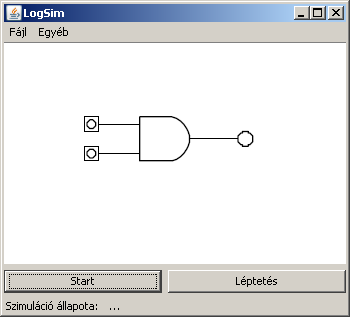
\includegraphics[width=4.25in]{chapters/chapter11/screenshots/felulet.png}
\caption{Főablak}
\label{fig:main}
\end{center}
\end{figure}

\begin{figure}[h]
\begin{center}
\includegraphics[width=1.98in]{chapters/chapter11/screenshots/menus1.png}
\includegraphics[width=0.83in]{chapters/chapter11/screenshots/menus2.png}
\caption{Fájl és az Egyéb menü almenüi}
\label{fig:menus}
\end{center}
\end{figure}

\begin{figure}[h]
\begin{center}
\includegraphics[width=2.8125in]{chapters/chapter11/screenshots/about.png}
\caption{Névjegy}
\label{fig:about}
\end{center}
\end{figure}

\section{A grafikus rendszer architektúrája}
\comment{A felület működésének elve, a grafikus rendszer architektúrája (struktúra diagramok). A struktúra diagramokon a prototípus azon és csak azon osztályainak is szerepelnie kell, amelyekhez a grafikus felületet létrehozó osztályok kapcsolódnak.}

\subsection{A felület működési elve}
\comment{Le kell írni, hogy a grafikai megjelenésért felelős osztályok, objektumok hogyan kapcsolódnak a meglevő rendszerhez, a megjelenítés során mi volt az alapelv. Törekedni kell az MVC megvalósításra. Alapelvek lehetnek: \textbf{push} alapú: a modell értesíti a felületet, hogy változott; \textbf{pull} alapú: a felület kérdezi le a modellt, hogy változott-e; \textbf{kevert}: a kettő kombinációja.}

Az általunk elkészített grafikus felület "pull" típusú, vagyis a grafikus rendszer kérdezi le a modell objektumoktól az aktuális állapotukat.
Azokhoz a modellobjektumokhoz, melyeket megjelenítünk, elkészítettünk egy-egy wrapper osztályt, mely a megjelenítésért és a megjelenítéshez szükséges információk tárolásáért felel. 
Az áramkört egy JPanel-ra rajzoljuk, mely biztosítja számunkra, hogy az elhelyezhető legyen bármilyen ablakon. Áramkör újrarajzoláskor, az eltárolt objektumok egyenkét rajzolják ki magukat az előzöleg megadott koordináták alapján.
Bármilyen felhasználói interakciónál, melynél változhat az áramkör állapota, az egész áramkört újrarajzoljuk, biztosítva ezzel, hogy a kirajzolt áramkör mindig az aktuális állapotban legyen megjelenítve.



\subsection{A felület osztály-struktúrája}
\comment{Osztálydiagram. Minden új osztály, és azon régiek, akik az újakhoz közvetlenül kapcsolódnak.}

\section{A grafikus objektumok felsorolása}
\comment{Az új osztályok felsorolása. Az régi osztályok közül azoknak a felsorolása, ahol változás volt. Ezek esetén csak a változásokat kell leírni.}

\subsection{Osztály1}
\begin{itemize}
\item Felelősség\newline
\comment{Mi az osztály felelőssége. Kb 1 bekezdés. Ha szükséges, akkor state-chart is.}
\item Ősosztályok\newline
\comment{Mely osztályokból származik (öröklési hierarchia)\newline
Legősebb osztály $\rightarrow$ Ősosztály2 $\rightarrow$ Ősosztály3...}
\item Interfészek\newline
\comment{Mely interfészeket valósítja meg.}
\item Attribútumok\newline
\comment{Milyen attribútumai vannak}
	\begin{itemize}
		\item attribútum1: attribútum jellemzése: mire való, láthatósága (UML jelöléssel), típusa
		\item attribútum2: attribútum jellemzése: mire való, láthatósága (UML jelöléssel), típusa
	\end{itemize}
\item Metódusok\newline
\comment{Milyen publikus, protected és privát  metódusokkal rendelkezik. Metódusonként precíz leírás, ha szükséges, activity diagram is  a metódusban megvalósítandó algoritmusról.}
	\begin{itemize}
		\item int foo(Osztály3 o1, Osztály4 o2): metódus leírása, láthatósága (UML jelöléssel)
		\item int bar(Osztály5 o1): metódus leírása, láthatósága (UML jelöléssel)
	\end{itemize}
\end{itemize}

\subsection{Osztály2}
\begin{itemize}
\item Felelősség\newline
\comment{Mi az osztály felelőssége. Kb 1 bekezdés. Ha szükséges, akkor state-chart is.}
\item Ősosztályok\newline
\comment{Mely osztályokból származik (öröklési hierarchia)\newline
Legősebb osztály $\rightarrow$ Ősosztály2 $\rightarrow$ Ősosztály3...}
\item Interfészek\newline
\comment{Mely interfészeket valósítja meg.}
\item Attribútumok\newline
\comment{Milyen attribútumai vannak}
	\begin{itemize}
		\item attribútum1: attribútum jellemzése: mire való, láthatósága (UML jelöléssel), típusa
		\item attribútum2: attribútum jellemzése: mire való, láthatósága (UML jelöléssel), típusa
	\end{itemize}
\item Metódusok\newline
\comment{Milyen publikus, protected és privát  metódusokkal rendelkezik. Metódusonként precíz leírás, ha szükséges, activity diagram is  a metódusban megvalósítandó algoritmusról.}
	\begin{itemize}
		\item int foo(Osztály3 o1, Osztály4 o2): metódus leírása, láthatósága (UML jelöléssel)
		\item int bar(Osztály5 o1): metódus leírása, láthatósága (UML jelöléssel)
	\end{itemize}
\end{itemize}

\section{Kapcsolat az alkalmazói rendszerrel}
\comment{Szekvencia-diagramokon ábrázolni kell a grafikus rendszer működését. Konzisztens kell legyen az előző alfejezetekkel. Minden metódus, ami ott szerepel, fel kell tűnjön valamelyik szekvenciában. Minden metódusnak, ami szekvenciában szerepel, szereplnie kell a valamelyik osztálydiagramon.}

\begin{figure}[h]
\begin{center}
\includegraphics[width=17cm]{chapters/chapter11/pdfs/1_program_start.pdf}
\caption{Program indítása}
\label{fig:program_start}
\end{center}
\end{figure}

\begin{figure}[h]
\begin{center}
\includegraphics[width=17cm]{chapters/chapter11/pdfs/2_loadcircuit.pdf}
\caption{Áramkör betöltése}
\label{fig:loadcircuit}
\end{center}
\end{figure}
%% Szglab4
% ===========================================================================
%
\section{Napló}

\begin{naplo}

\bejegyzes
{2011.04.20.~14:00~} % Kezdet
{3 óra} % Időtartam
{Dévényi A.\newline
Jákli G.\newline
Kriván B.} % Résztvevők
{Értekezlet.\newline
Megbeszéltük a grafikus felületet, osztályokat és a szekvenciákat.
Döntés: szétosztottuk a diagramokat} % Leírás

\bejegyzes
{2011.04.23.~11:30~}
{45 perc}
{Kriván B.}
{A grafikus interfész c. fejezet elkészítése}


\end{naplo}


%%
%\setcounter{chapter}{12}
%% Szglab4
% ===========================================================================
%
\chapter{Grafikus felület specifikációja}

\thispagestyle{fancy}

\section{Fordítási és futtatási útmutató}

\subsection{Fájllista}

\begin{fajllista}

\fajl
{src/logsim/\newline
ComponentViewCreator.java} % Kezdet
{4506 byte} % Idptartam
{2011.05.01.~14:33~} % Résztvevők
{Minden áramköri elemhez létrehoz egy megjeleníthető elemet} % Leírás

\fajl
{src/logsim/Config.java} % Kezdet
{4195 byte} % Idptartam
{2011.05.01.~14:33~} % Résztvevők
{A kapcsolók és szekvenciagenerátorok kimentéséért és betöltéséért felelős} % Leírás

\fajl
{src/logsim/Controller.java} % Kezdet
{1600 byte} % Idptartam
{2011.05.01.~14:33~} % Résztvevők
{A vezérlés interfészét tartalmazza} % Leírás

\fajl
{src/logsim/GuiController.java} % Kezdet
{12086 byte} % Idptartam
{2011.05.01.~14:33~} % Résztvevők
{A szimuláció működéséért felelős; felhasználói utasítások értelmezése} % Leírás

\fajl
{src/logsim/Parser.java} % Kezdet
{13730 byte} % Idptartam
{2011.05.01.~14:33~} % Résztvevők
{Az áramkörleíró fájl feldolgozását végzi} % Leírás

\fajl
{src/logsim/model/Circuit.java} % Kezdet
{1096 byte} % Idptartam
{2011.05.01.~14:33~} % Résztvevők
{Áramkört reprezentáló osztály} % Leírás

\fajl
{src/logsim/model/\newline
Simulation.java} % Kezdet
{857 byte} % Idptartam
{2011.05.01.~14:33~} % Résztvevők
{Egy szimulációt reprezentáló osztály} % Leírás

\fajl
{src/logsim/model/Value.java} % Kezdet
{714 byte} % Idptartam
{2011.05.01.~14:33~} % Résztvevők
{Az áramkörben előforduló értkékeket tartalmazó osztály} % Leírás

\fajl
{src/logsim/model/component/\newline
AbstractComponent.java} % Kezdet
{4612 byte} % Idptartam
{2011.05.01.~14:33~} % Résztvevők
{Az alkatrészek absztrakt ősosztálya} % Leírás

\fajl
{src/logsim/model/component/\newline
Composite.java} % Kezdet
{15419 byte} % Idptartam
{2011.05.09.~10:35~} % Résztvevők
{A kompozit elem leírása} % Leírás

\fajl
{src/logsim/model/component/\newline
DisplayComponent.java} % Kezdet
{644 byte} % Idptartam
{2011.05.01.~14:33~} % Résztvevők
{Megjelenítő típusú alkatrészek absztrakt ősosztálya} % Leírás

\fajl
{src/logsim/model/component/\newline
FlipFlop.java} % Kezdet
{1799 byte} % Idptartam
{2011.05.09.~10:35~} % Résztvevők
{Flipflop típusú alkatrészek absztrakt ősosztálya} % Leírás

\fajl
{src/logsim/model/component/\newline
Pin.java}
{612 byte}
{2011.05.01.~14:33~}
{A kimeneteket és bemeneteket tároló osztály}

\fajl
{src/logsim/model/component/\newline
SourceComponent.java} % Kezdet
{1074 byte} % Idptartam
{2011.05.01.~14:33~} % Résztvevők
{Forrás típusú alkatrészek absztrakt ősosztálya} % Leírás

\fajl
{src/logsim/model/component/\newline
Wire.java} % Kezdet
{1109 byte} % Idptartam
{2011.05.01.~14:33~} % Résztvevők
{Vezetéket megvalósító osztály} % Leírás

\fajl
{src/logsim/model/component/\newline
impl/AndGate.java} % Kezdet
{1124 byte} % Idptartam
{2011.05.01.~14:33~} % Résztvevők
{Az ÉS kapu alkatrészt megvalósító osztály} % Leírás

\fajl
{src/logsim/model/component/\newline
impl/FlipFlopD.java} % Kezdet
{1178 byte} % Idptartam
{2011.05.09.~10:35~} % Résztvevők
{A D flipflop alkatrészt megvalósító osztály} % Leírás

\fajl
{src/logsim/model/component/\newline
impl/FlipFlopJK.java} % Kezdet
{1800 byte} % Idptartam
{2011.05.09.~10:35~} % Résztvevők
{A JK flipflop alkatrészt megvalósító osztály} % Leírás

\fajl
{src/logsim/model/component/\newline
impl/Gnd.java} % Kezdet
{774 byte} % Idptartam
{2011.05.01.~14:33~} % Résztvevők
{A permanens logikai nullát megvalósító osztály} % Leírás

\fajl
{src/logsim/model/component/\newline
impl/Inverter.java} % Kezdet
{847 byte} % Idptartam
{2011.05.01.~14:33~} % Résztvevők
{Az inverter alkatrészt megvalósító osztály} % Leírás

\fajl
{src/logsim/model/component/\newline
impl/Led.java} % Kezdet
{924 byte} % Idptartam
{2011.05.01.~14:33~} % Résztvevők
{A led megjelenítőt megvalósító osztály} % Leírás

\fajl
{src/logsim/model/component/\newline
impl/Mpx.java} % Kezdet
{1431 byte} % Idptartam
{2011.05.01.~14:33~} % Résztvevők
{A multiplexer alkatrészt megvalósító osztály} % Leírás

\fajl
{src/logsim/model/component/\newline
impl/Node.java} % Kezdet
{1221 byte} % Idptartam
{2011.05.01.~14:33~} % Résztvevők
{Csomópont alkatrészt megvalósító osztály} % Leírás

\fajl
{src/logsim/model/component/\newline
impl/OrGate.java} % Kezdet
{1194 byte} % Idptartam
{2011.05.01.~14:33~} % Résztvevők
{a VAGY kapu alkatrészt megvalósító osztály} % Leírás

\fajl
{src/logsim/model/component/\newline
impl/Scope.java} % Kezdet
{1663 byte} % Idptartam
{2011.05.01.~14:33~} % Résztvevők
{Oszcilloszkópot megvalósító osztály} % Leírás

\fajl
{src/logsim/model/component/\newline
impl/SequenceGenerator.java} % Kezdet
{2532 byte} % Idptartam
{2011.05.01.~14:33~} % Résztvevők
{A szekvenciagenerátor alkatrészt megvalósító osztály} % Leírás

\fajl
{src/logsim/model/component/\newline
impl/SevenSegmentDisplay.java} % Kezdet
{1176 byte} % Idptartam
{2011.05.01.~14:33~} % Résztvevők
{A 7 szegmenses kijelző alkatrészt megvalósító osztály} % Leírás

\fajl
{src/logsim/model/component/\newline
impl/Toggle.java} % Kezdet
{1719 byte} % Idptartam
{2011.05.01.~14:33~} % Résztvevők
{A kapcsolót megvalósító osztály} % Leírás

\fajl
{src/logsim/model/component/\newline
impl/Vcc.java} % Kezdet
{746 byte} % Idptartam
{2011.05.01.~14:33~} % Résztvevők
{A permanens logikai egyet megvalósító osztály} % Leírás

\fajl
{src/logsim/view/\newline
CircuitView.java}
{3551 byte}
{2011.05.01.~14:33~}
{Áramkört kirajzoló panel.}

\fajl
{src/logsim/view/\newline
DrawableView.java}
{555 byte}
{2011.05.01.~14:33~}
{Áramköri panelre rajzolható objektum.}

\fajl
{src/logsim/view/\newline
Frame.form}
{23241 byte}
{2011.05.01.~14:33~}
{A főablak elemeinek elrendezését tartalmazó fájl.}

\fajl
{src/logsim/view/\newline
Frame.java}
{28642 byte}
{2011.05.09.~11:34~}
{A főablak elemeinek interakcióinak feldolgozásáért felelős osztály.}

\fajl
{src/logsim/view/\newline
FrameView.java}
{1914 byte}
{2011.05.01.~14:33~}
{Főablak interfésze.}

\fajl
{src/logsim/view/component\newline
ComponentView.java}
{2620 byte}
{2011.05.01.~14:33~}
{Az elemek megjelenítéséért felelős osztályok abszrakt ősosztálya.}

\fajl
{src/logsim/view/component\newline
WireView.java}
{2050 byte}
{2011.05.01.~14:33~}
{A kábelek kirajzolását végző osztály.}

\fajl
{src/logsim/view/component/\newline
impl/AndGateView.java} % Kezdet
{1446 byte} % Idptartam
{2011.05.01.~14:33~} % Résztvevők
{Az ÉS kapu alkatrészt megjelenítő osztály} % Leírás

\fajl
{src/logsim/view/component/\newline
impl/CompositeView.java}
{1758 byte}
{2011.05.09.~10:48~}
{A kompozit alkatrészt megjelenítő osztály}

\fajl
{src/logsim/view/component/\newline
impl/FlipFlopDView.java} % Kezdet
{1257 byte} % Idptartam
{2011.05.01.~14:33~} % Résztvevők
{A D flipflop alkatrészt megjelenítő osztály} % Leírás

\fajl
{src/logsim/view/component/\newline
impl/FlipFlopJKView.java} % Kezdet
{1272 byte} % Idptartam
{2011.05.01.~14:33~} % Résztvevők
{A JK flipflop alkatrészt megjelenítő osztály} % Leírás

\fajl
{src/logsim/view/component/\newline
impl/GndView.java} % Kezdet
{1128 byte} % Idptartam
{2011.05.01.~14:33~} % Résztvevők
{A permanens logikai nullát megjelenítő osztály} % Leírás

\fajl
{src/logsim/view/component/\newline
impl/InverterView.java} % Kezdet
{1425 byte} % Idptartam
{2011.05.01.~14:33~} % Résztvevők
{Az inverter alkatrészt megjelenítő osztály} % Leírás

\fajl
{src/logsim/view/component/\newline
impl/LedView.java} % Kezdet
{1400 byte} % Idptartam
{2011.05.01.~14:33~} % Résztvevők
{A led megjelenítőt megjelenítő osztály} % Leírás

\fajl
{src/logsim/view/component/\newline
impl/MpxView.java} % Kezdet
{1187 byte} % Idptartam
{2011.05.01.~14:33~} % Résztvevők
{A multiplexer alkatrészt megjelenítő osztály} % Leírás

\fajl
{src/logsim/view/component/\newline
impl/NodeView.java} % Kezdet
{2013 byte} % Idptartam
{2011.05.09.~10:35~} % Résztvevők
{Csomópont alkatrészt megjelenítő osztály} % Leírás

\fajl
{src/logsim/view/component/\newline
impl/OrGateView.java} % Kezdet
{1284 byte} % Idptartam
{2011.05.01.~14:33~} % Résztvevők
{a VAGY kapu alkatrészt megjelenítő osztály} % Leírás

\fajl
{src/logsim/view/component/\newline
impl/ScopeView.java} % Kezdet
{1479 byte} % Idptartam
{2011.05.01.~14:33~} % Résztvevők
{Oszcilloszkópot megjelenítő osztály} % Leírás

\fajl
{src/logsim/view/component/\newline
impl/SequenceGeneratorView.java} % Kezdet
{1603 byte} % Idptartam
{2011.05.01.~14:33~} % Résztvevők
{A szekvenciagenerátor alkatrészt megjelenítő osztály} % Leírás

\fajl
{src/logsim/view/component/\newline
impl/SevenSegmentDisplayView.java} % Kezdet
{3749 byte} % Idptartam
{2011.05.01.~14:33~} % Résztvevők
{A 7 szegmenses kijelző alkatrészt megjelenítő osztály} % Leírás

\fajl
{src/logsim/view/component/\newline
impl/ToggleView.java} % Kezdet
{1549 byte} % Idptartam
{2011.05.01.~14:33~} % Résztvevők
{A kapcsolót megjelenítő osztály} % Leírás

\fajl
{src/logsim/view/component/\newline
impl/VccView.java} % Kezdet
{1104 byte} % Idptartam
{2011.05.01.~14:33~} % Résztvevők
{A permanens logikai egyet megjelenítő osztály} % Leírás

\fajl
{compile.bat}
{183 byte}
{2011.05.09.~10:48~}
{Fordítást segítő .bat fájl}

\fajl
{doc.bat}
{314 byte}
{2011.05.09.~10:35~}
{Java dokumentációt generáló .bat fájl}

\fajl
{run.bat}
{111 byte}
{2011.05.09.~10:56~}
{Futtatást segítő .bat fájl}

\fajl
{tesztek/test1.txt} % Kezdet
{78 byte} % Idptartam
{2011.04.17.~21:58~} % Résztvevők
{Az 1. teszteset áramköre} % Leírás

\fajl
{tesztek/test2.txt} % Kezdet
{221 byte} % Idptartam
{2011.04.17.~21:58~} % Résztvevők
{A 2. teszteset áramköre} % Leírás

\fajl
{tesztek/test3.txt} % Kezdet
{83 byte} % Idptartam
{2011.04.17.~21:58~} % Résztvevők
{A 3. teszteset áramköre} % Leírás

\fajl
{tesztek/test4.txt} % Kezdet
{96 byte} % Idptartam
{2011.04.17.~21:58~} % Résztvevők
{A 4. teszteset áramköre} % Leírás

\fajl
{tesztek/test5.txt} % Kezdet
{89 byte} % Idptartam
{2011.04.17.~21:58~} % Résztvevők
{Az 5. teszteset áramköre} % Leírás

\fajl
{tesztek/test6.txt} % Kezdet
{263 byte} % Idptartam
{2011.04.17.~21:58~} % Résztvevők
{A 6. teszteset áramköre} % Leírás

\fajl
{tesztek/test7.txt} % Kezdet
{161 byte} % Idptartam
{2011.04.17.~21:58~} % Résztvevők
{A 7. teszteset áramköre} % Leírás

\end{fajllista}

\subsection{Fordítás}
A hibamentes és minél inkább gördülékeny fordítás érdekében létrehoztunk egy \texttt{compile.bat} nevezetű batch fájlt, mely a projekt főkönyvtárában található. Projekt főkönytára az, amelyik a batch fájlokat és a "src" nevezetű mappát tartalmazza, melyben a program forráskódja található. Szükség estén kézzel kell módosítani a batch fájl
\begin{verbatim}
set C="C:\Program Files\Java\jdk1.6.0_23\bin\"
\end{verbatim}
sorát, attól függően, hogy a gépen éppen melyik Java JDK verzió található és az hová van telepítve!\\
A \texttt{compile.bat} fájl az alábbi parancsokat hajtja végre:
\lstinputlisting[escapeinside=`', xleftmargin=10pt, frame=single, basicstyle=\ttfamily\footnotesize, language=sh]{../LogSimGui/compile.bat}
Ha hibamentes volt a fordítás, a "Fordítás sikeres" kimenettel értesíti a felhasználót.\\
A fordítás sikeressége után, lehetőség van a dokumentáció legenerálására is. Ehhez felhasználható a főkönyvtárban található \texttt{doc.bat} batch fájl.
Szükség estén kézzel kell módosítani a batch file \begin{verbatim}
set C="C:\Program Files\Java\jdk1.6.0_23\bin\"
\end{verbatim}
sorát, attól függően, hogy a gépen éppen melyik Java JDK verzió található és az hová van telepítve!\\
A batch fájl az alábbi parancsokat hajtja végre:
\lstinputlisting[escapeinside=`', xleftmargin=10pt, frame=single, basicstyle=\ttfamily\footnotesize, language=sh]{../LogSimGui/doc.bat}
Ha a dokumentum generálás sikeres volt, akkor a documents nevezetű mappában megtaláhatóak a kívánt dokumentumok.
\subsection{Futtatás}
A futtatás megkönnyítése érdekében elkészítettük a \texttt{run.bat} batch fájlt.
Szükség estén kézzel kell módosítani a \texttt{run.bat} batch fájlt
\begin{verbatim}
set C="C:\Program Files\Java\jdk1.6.0_23\bin\"
\end{verbatim} sorát, attól függően, hogy a gépen éppen melyik Java JDK verzió található és az hová van telepítve!\\
A \texttt{run.bat} fájl az alábbi parancsokat hajtja végre:
\lstinputlisting[escapeinside=`', xleftmargin=10pt, frame=single, basicstyle=\ttfamily\footnotesize, language=sh]{../LogSimGui/run.bat}
A "build" könyvtárból elindítja az előzőleg lefordított programot.

\section{Értékelés}

\begin{ertekeles}
\tag{Apagyi Gábor}
{13}
\tag{Dévényi Attila}
{20}
\tag{Jákli Gábor}
{21}
\tag{Kriván Bálint}
{34}
\tag{Péter Tamás Pál}
{13}
\end{ertekeles}

%% Szglab4
% ===========================================================================
%
\section{Napló}

\begin{naplo}

\bejegyzes
{2010.03.21.~18:00~} % Kezdet
{2,5 óra} % Időtartam
{Horváth\newline
Németh\newline
Tóth\newline
Oláh} % Résztvevők
{Értekezlet. Döntés: Horváth elkészíti az osztálydiagramot, Oláh a use-case leírásokat.} % Leírás

\bejegyzes
{2010.03.23.~23:00~}
{5 óra}
{Németh}
{Tevékenység: Németh implementálja a tesztelő programokat.}

\bejegyzes
{...}
{...}
{...}
{...}


\end{naplo}


%%
%\setcounter{chapter}{13}
%% Szglab4
% ===========================================================================
%
\chapter{Összefoglalás}

\thispagestyle{fancy}

\section{Projekt összegzés}
\comment{A projekt tapasztalatait összegző részben a csapatoknak a projektről kialakult véleményét várjuk. A megválaszolandók köre az alábbi. }

\begin{munka}
\munkaido{Apagyi Gábor}{23}
\munkaido{Dévényi Attila}{35}
\munkaido{Jákli Gábor}{37}
\munkaido{Kriván Bálint}{61}
\munkaido{Péter Tamás Pál}{22.5}
\osszesmunkaido{178.5}
\end{munka}

\begin{forrassor}
\munkaido{Szkeleton}{1735}
\munkaido{Protó}{2571}
\munkaido{Grafikus}{5023}
\end{forrassor}

\begin{itemize}
\item Mit tanultak a projektből konkrétan és általában? \newline

Végre gyakorlatban is láthattuk azt, amit az előző félévben a Szoftvertechnológia tárgyból tanultunk. Kipróbálhattuk magunkat egy viszonylag hosszabb projektmunkában, megismerhettük egymás erősségeit és gyengeségeit. 

\item Mi volt a legnehezebb és a legkönnyebb? \newline

Legnehezebb a közös időpontok megszervezése, valamint a közös tervezések közben felmerült problémák megoldásainak közös elfogadása. A legkönnyebb az implementálás volt az elkészült tervek alapján, mely szinte csak gépelésről szólt.

\item Összhangban állt-e az idő és a pontszám az elvégzendő feladatokkal? \newline

Az első részben kicsit tévútra indultunk és ott fölösleges órák mentek el a rossz megoldásra, de ezt a negyedik beadásra sikerült korrigálni. Összességben korrektnek érezzük a kapott pontszámokat.

\item Ha nem, akkor hol okozott ez nehézséget? \newline

Ahogy már említettük az első részben az analízis modell rosszra sikeredett, ezt sok idő volt korrigálni, és maga a rossz megoldás is sok időt elvett.

\item Milyen változtatási javaslatuk van? \newline

Több évfolyamtárstól hallottuk, hogy labvezérek által számonkért beadandó dokumentumok minőségének a szórása igen nagy. Mi úgy érezzük, hogy beletettünk elég sok munkát és ennek megfelelően jogosnak érezzük az elért eredményeket, pontszámokat, azonban néhány másik csoport ennek töredékéért megkapja ugyanazt, vagy akár többet, annak ellenére, hogy nem biztos, hogy jobb minőségű munkát adtak ki a kezükből. Ha ezen egy kicsit lehetne javítani, homogenizálni a labvezérek egyéni elvárásait, akkor talán kicsit jobb lenne a több munkát belefektető csapatok hangulata. Továbbá ha megnézzük az eltöltött órák számát, akkor kicsit kevésnek érezzük a tárgyért járó 2 kreditet, 3-nak esetleg 4-nek jobban örülnénk.

\item Milyen feladatot ajánlanának a projektre? \newline

Mindenképpen valami ehhez hasonlót, tehát a projekt végére egy ,,használható'' termék-szerűség készüljön el, amit akár valódi célokra is fel lehet használni (gondolok itt arra, hogy például a most elkészült programot a Digitális technika I-II. című tárgy keretében akár még használni is lehetne).

\end{itemize}

%
%\clearpage
%
% Függelék
%
%\appendix
\end{document}
%
% EOF
%
